\documentclass[11pt]{report}
\usepackage[margin=1.1in]{geometry}
\usepackage[utf8]{inputenc}
\usepackage[italian]{babel}
\usepackage{amssymb} 
\usepackage{amsmath}
\usepackage{amsthm}
\usepackage{multicol}
\usepackage{url}
\usepackage{pdfpages}
\usepackage{hyperref}


\renewcommand{\qed}{\hfill\blacksquare}

\setcounter{tocdepth}{3}
\setcounter{secnumdepth}{3}

\begin{document}
\title{Appunti su Assembler}
\author{Gabriele Frassi}
\date{A.A 2020-2021 - Primo semestre}
\maketitle

\small\tableofcontents\normalsize

\chapter{Unimap}
\small
\begin{enumerate}
\item \textbf{Mar 29/09/2020 11:45-13:45 (2:0 h)} lezione: Lezione: Introduzione al corso ed informazioni pratiche. Richiami sulla rappresentazione dei numeri naturali ed interi in base 2. Schema a blocchi del calcolatore: memoria, spazio di I/O, processore. I registri del processore, condizioni al reset. (GIOVANNI STEA)
\item \textbf{Mer 30/09/2020 10:45-12:45 (2:0 h)} lezione: Codifica macchina e codifica mnemonica delle istruzioni e primo esempio di programma in Assembler. Indirizzamento degli operandi nelle istruzioni operative. Istruzioni di trasferimento (inizio). (GIOVANNI STEA)
\item \textbf{Gio 01/10/2020 10:45-12:45 (2:0 h)} lezione: Istruzioni di trasferimento (fine). Istruzioni aritmetiche (inizio). (GIOVANNI STEA)
\item \textbf{Ven 02/10/2020 15:00-17:00 (2:0 h)} lezione: istruzioni aritmetiche (fine). Istruzioni di traslazione e rotazione. Istruzioni logiche. Istruzioni di controllo. (GIOVANNI STEA)
\item \textbf{Mar 06/10/2020 11:45-13:45 (2:0 h)} lezione: Programmare in linguaggio Assembler: struttura sintattica di un programma. Direttive in Assembler: dichiarazione di variabile e di costante. Strutture di controllo di flusso tipiche dei linguaggi ad alto livello e loro traduzione in linguaggio Assembler. (GIOVANNI STEA)
\item \textbf{Mer 07/10/2020 10:45-12:45 (2:0 h)} esercitazione: (in copresenza con Ing. R. Zippo) Esercitazione Assembler. Presentazione ambiente di sviluppo. Uso del debugger per verifica del programma e controllo degli errori. (GIOVANNI STEA)
\item \textbf{Gio 08/10/2020 10:45-12:45 (2:0 h)} lezione: Sottoprogrammi e passaggio dei parametri. Gestione della pila. I/O e sottoprogrammi di ingresso/uscita. Istruzioni stringa. (GIOVANNI STEA)
\item \textbf{Ven 09/10/2020 15:00-17:00 (2:0 h)} lezione: Note sulla programmazione Assembler. Generalità sulle reti logiche. Modello, limiti del modello e non contemporaneità. descrizione mediante tabelle di verita'. Esempi di reti combinatorie semplici. AND e OR a piu' di due ingressi. Algebra di Boole (GIOVANNI STEA)
\item \textbf{Ven 16/10/2020 15:00-17:00 (2:0 h)} esercitazione: Esercitazione: (in copresenza con Ing. R. Zippo) Esercitazione Assembler. Svolgimento di esercizi di programmazione. (GIOVANNI STEA)
\item \textbf{Ven 23/10/2020 15:00-17:00 (2:0 h)} esercitazione: (in copresenza con Ing. R. Zippo) Esercitazione Assembler. Svolgimento di esercizi di programmazione. (GIOVANNI STEA)
\end{enumerate}
\normalsize
\part{Lezioni di Stea}



\chapter{Martedì 29/09/2020}


\section{Linguaggio assembler}
\paragraph{Nome preciso} Il nome preciso è \emph{Assembly}, ma lo chiameremo \emph{Assembler} per ragioni storiche (a Pisa è sempre stato chiamato così)
\paragraph{Differenza da altri linguaggi} Il linguaggio Assembler è di basso livello, in contrapposizione al C++ che è di alto livello. Con questo linguaggio saremo in grado di scrivere \textbf{istruzioni macchina} eseguite dal processore.
\begin{itemize}
\item Con linguaggio ad alto livello intendiamo un linguaggio i cui costrutti sono più vicini al ragionamento dell'essere umano
\item Con linguaggio a basso livello intendiamo un linguaggio i cui costrutti sono più vicini al ragionamento della macchina.
\end{itemize}
Scrivere in assembler significa imparare a ragionare come la macchina!

\paragraph{Sintassi simbolica} Con Assembler non scriveremo in linguaggio macchina (sequenze di zeri e uno incomprensibili per l'uomo), ma ricorreremo a una sintassi simbolica. Qual è la differenza?
\begin{itemize}
\item In C++ il compilatore effettua una traduzione vera e propria. Basti pensare che dietro l'istruzione
\begin{verbatim}
a=b;
\end{verbatim}
possono celarsi centinaia di istruzioni macchina.
\item In Assembler abbiamo l'\textbf{assemblaggio}, svolto dall'assemblatore.  Ponendo quanto segue
\begin{verbatim}
MOV %AX, %BX
\end{verbatim}
rappresentiamo un numero binario. Questa è una traduzione $1:1$!
\end{itemize}
\paragraph{Ulteriori differenze rispetto al C++}
\begin{itemize}
\item Non sono presenti i cosiddetti \emph{costrutti di flusso strutturato}: for, while, dowhile, ifthenelse, case. Saranno presenti istruzioni di salto \emph{jump}.
\item Le variabili non hanno un tipo. Avremo stringhe di bit. Cosa rappresenti una variabile è pensiero esclusivamente nostro, non della macchina
\end{itemize}
\paragraph{Assembler processor-specific} L'assembler è specifico per ogni processore: i comandi possono cambiare. Segue che non sia un linguaggio, portabile, a differenza del C++ o dei linguaggi che impareremo simultaneamente a progettazione web. Utilizzeremo, in questo corso, assembler per \emph{Intel x86}, visto la validità dei suoi principi per quasi tutte le versioni di Assembler. Non lo studieremo tutto, considerando la vastità del manuale (20 ore per 2000 pagine? impensabile)
\paragraph{Utilità di Assembler} Assembler è utilizzato per \emph{sistemi Embedded}. Al di là di questo un ingegnere informatico deve sapere come si comporta un processore!
\section{Struttura di un calcolatore}
Un calcolatore può essere immaginato come una serie di blocchi connessi da una \emph{rete di interconnessione} detta \textbf{bus}. In particolare individuiamo nello schema funzionale:
\begin{center}
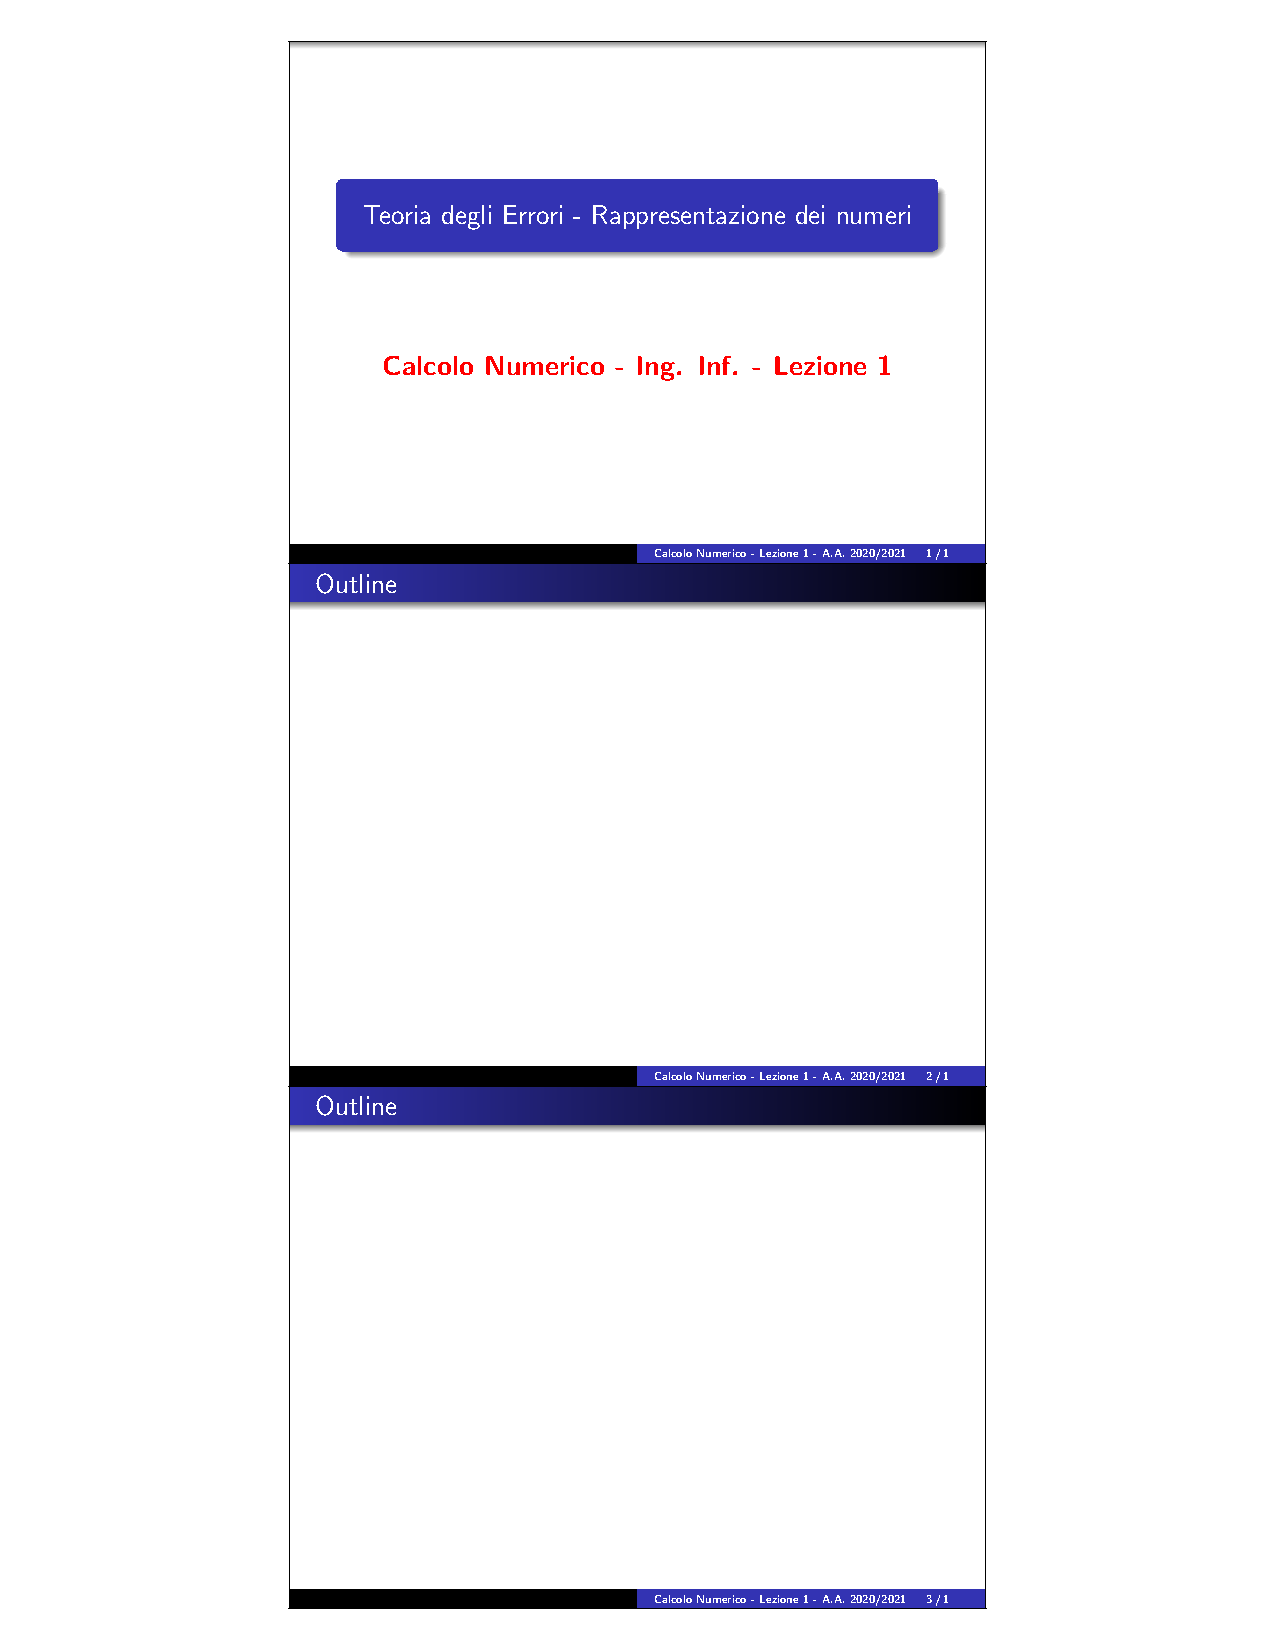
\includegraphics{img/1.PNG}
\end{center}
\begin{enumerate}
\item \textbf{Sottosistema di ingresso/uscita}: area che si occupa di compiere la traduzione dal mondo esterno al calcolatore e viceversa. Immagini, suoni, qualunque contenuto vengono codificate in stringhe di bit. Nella stessa area abbiamo il dispositivo (che non è detto faccia sia input che output, pensiamo alla tastiera e al mouse): questo non è collegato direttamente al bus, ma passa per \emph{interfacce}, reti logiche che adattano il dispositivo al bus (attraverso protocolli il calcolatore può interfacciarsi con i dispositivi senza conoscerne la struttura fisica)
\item \textbf{Memoria principale}: ospita i programmi (le istruzioni da eseguire) e i dati (non tutti, alcuni di questi potrebbero trovarsi nel sottosistema introdotto prima)
\item \textbf{Processore}: contiene al suo interno almeno le seguenti unità:
\begin{itemize}
\item la ALU (\emph{Arithmetic Logic Unit}): unità che si occupa di eseguire istruzioni logiche (AND, OR e NOT) e aritmetiche (relativamente a numeri naturali e interi)
\item la FPU (\emph{Floating Point Unit}): unità che svolge istruzioni aritmetiche relative ai numeri reali
\end{itemize}
\end{enumerate}
\paragraph{Cosa fa il processore} Il processore, ciclicamente:
\begin{itemize}
\item preleva un'istruzione macchina dalla memoria
\item la esegue
\end{itemize}

\section{Ripasso: rappresentazione dell'informazione}
\subsection{Numeri naturali}
Con $N$ bit possiamo rappresentare $2^N$ numeri naturali, precisamente quelli compresi nell'intervallo $[0, 2^N-1]$. Come nella base 10 anche qua abbiamo un sistema basato sulla presenza di cifre più significative e cifre meno significative (rispettivamente MSB, \emph{Most significant bit}, e LSB, \emph{Least Significant Bit}). Un numero in base 2 avente la seguente forma
\[b_{N-1},b_{N-2},\dots,b_1,b_0\]
può essere rappresentato in base 10 mediante la seguente formula
\[X=\sum_{i=0}^{N-1}b_i\,2^i\]
ricordiamo, inoltre, l'algoritmo \textbf{DIV\&MOD} per convertire numeri dalla base 10 alla base 2 (vedere dispensa di Rappresentazione dell'informazione, FdP).
\subsection{Numeri interi}
Con $N$ bit possiamo rappresentare $2^N$ numeri interi, precisamente quelli compresi nell'intervallo $[-2^{N-1},2^{N-1}-1]$. Osserviamo che la cosa \underline{non} è simmetrica:
\begin{itemize}
\item Con $N=8$ abbiamo $[-128,127]$
\item Con $N=16$ abbiamo $[-32768,32767]$
\end{itemize}
\noindent La rappresentazione che ci interessa è quella \textbf{in complemento a 2}. Per ottenere un numero da base 10 a base 2 procederemo identificando la seguente stringa di bit $X$ (numeri naturali per rappresentare numeri interi)
\[X=\begin{cases}x&x \geq	 0\\2^N+x&x <0\end{cases}\;\;\;\text{purchè si abbia }x \in [-2^{N-1},2^{N-1}-1]\]
ricordiamo che la cosa deve essere verificata, il metodo ci porta ad ottenere una sequenza binaria in ogni caso. Se la condizione non è soddisfatta quella sequenza non rappresenta il numero da cui siamo partiti. Tutto questo può essere rappresentato anche così: $X=|x|_{2^N}$. Vedremo questa notazione nella parte di Aritmetica del corso.
\pagebreak
\subsubsection{Diagramma della farfalla}
Quanto detto prima può essere tradotto sfruttando la seguente immagine
\begin{center}
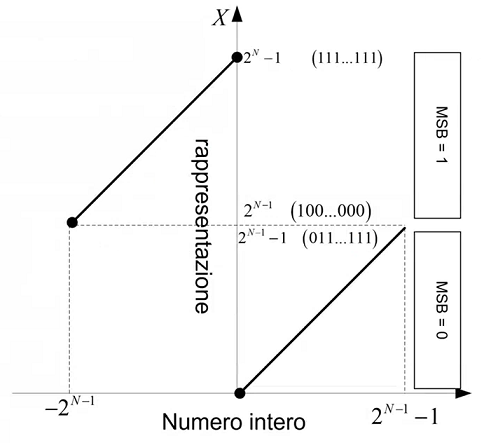
\includegraphics{img/2.PNG}
\end{center}
Lungo l'asse delle ascisse abbiamo gli interi $x$, lungo l'asse delle ordinate le stringhe di bit $X$ (naturali, capiremo per bene nella parte di Aritmetica).
Osserviamo che
\begin{itemize}
\item Nel semiasse positivo abbiamo una retta con coefficiente $m=1$ dove $X=x$. Quest'area consiste nei numeri positivi ed è quella con $\text{MSB}=0$
\item Nel semiasse negativo abbiamo una retta parallela alla precedente traslata di $2^N$ ($X=x+2^N$). Quest'area consiste nei numeri negativi ed è quella con $\text{MSB}=1$
\end{itemize}
Ricordiamo che l'ultimo numero con $MSB=0$ ($2^{N-1}-1$) sarà del tipo $011\dots 11$, mentre l'ultimo numero con $MSB=0$ ($2^N-1$) sarà del tipo $111\dots 11$. Dallo stesso disegno possiamo capire il processo inverso per passare da base 2 a base 10
\[x=\begin{cases}X&X_{N-1} = 0\\-(\overline{X}+1)&X_{N-1} = 1\end{cases}\]
ottengo il naturale \emph{complementando} i bit della rappresentazione (cioè invertendo gli zeri e gli uno). Spiegheremo questa cosa nella parte di Aritmetia del corso! Prendiamo il seguente esempio:
\begin{align*}&10110101\\-(&01001010+1)\\-(&01001011)=-(64+8+2+1)=-75\end{align*}

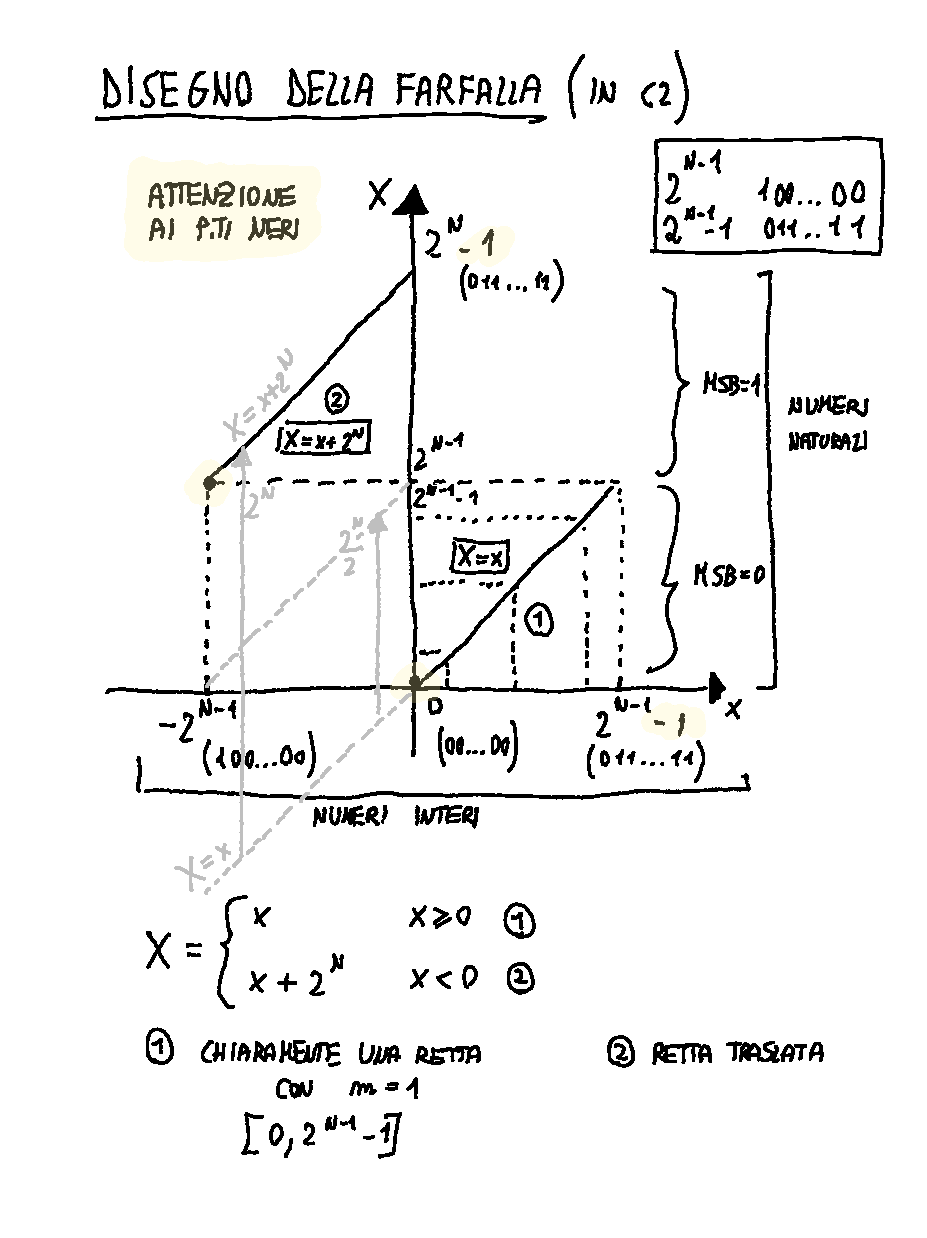
\includepdf[pagecommand={\thispagestyle{plain}},scale=0.92,pages=-]{pdf/disegnofarfallac2}

\subsubsection{Tabella di conversione da $-8$ a $+7$ in $p=4$}
\begin{center}
\begin{tabular}{ |c|c|c| }
 \hline 
$\mathbf{\mathbb{N}}$ & $\mathbf{A}$ & $\mathbf{a}$\\
\hline
 $0$ & $0000$  & $+0$\\ 
 \hline
 $1$ & $0001$  & $+1$\\ 
 \hline
 $2$ & $0010$  & $+2$\\ 
 \hline
 $3$ & $0011$  & $+3$\\ 
 \hline
 $4$ & $0100$  & $+4$\\ 
 \hline
 $5$ & $0101$  & $+5$\\ 
 \hline
 $6$ & $0110$  & $+6$\\ 
 \hline
 $7$ & $0111$  & $+7$\\ 
 \hline
 $8$ & $1000$  & $-8$\\ 
 \hline
 $9$ & $1001$  & $-7$\\ 
 \hline
 $10$ & $1010$  & $-6$\\ 
 \hline
 $11$ & $1011$  & $-5$\\ 
 \hline
 $12$ & $1100$  & $-4$\\ 
 \hline
 $13$ & $1101$  & $-3$\\ 
 \hline
 $14$ & $1110$  & $-2$\\ 
 \hline
 $15$ & $1111$  & $-1$\\ 
 \hline
\end{tabular}
\end{center} 
\subsubsection{Rappresentazione esadecimale}
Molto spesso le sequenze binarie sono lunghe e difficili da comprendere. Potremo compattare convertendo in base 10, ma questo richiede dei calcoli. Proprio per questo andiamo ad adottare la \textbf{notazione esadecimale}. $4$ bit consistono in un numero compreso tra $0$ e $15$, sfruttando una scorciatoia (descritta nella dispensa di rappresentazione dell'informazione, FdP) possiamo sostituire in modo rapido leggendo blocchi di cifre da destra verso sinistra.
\begin{center}
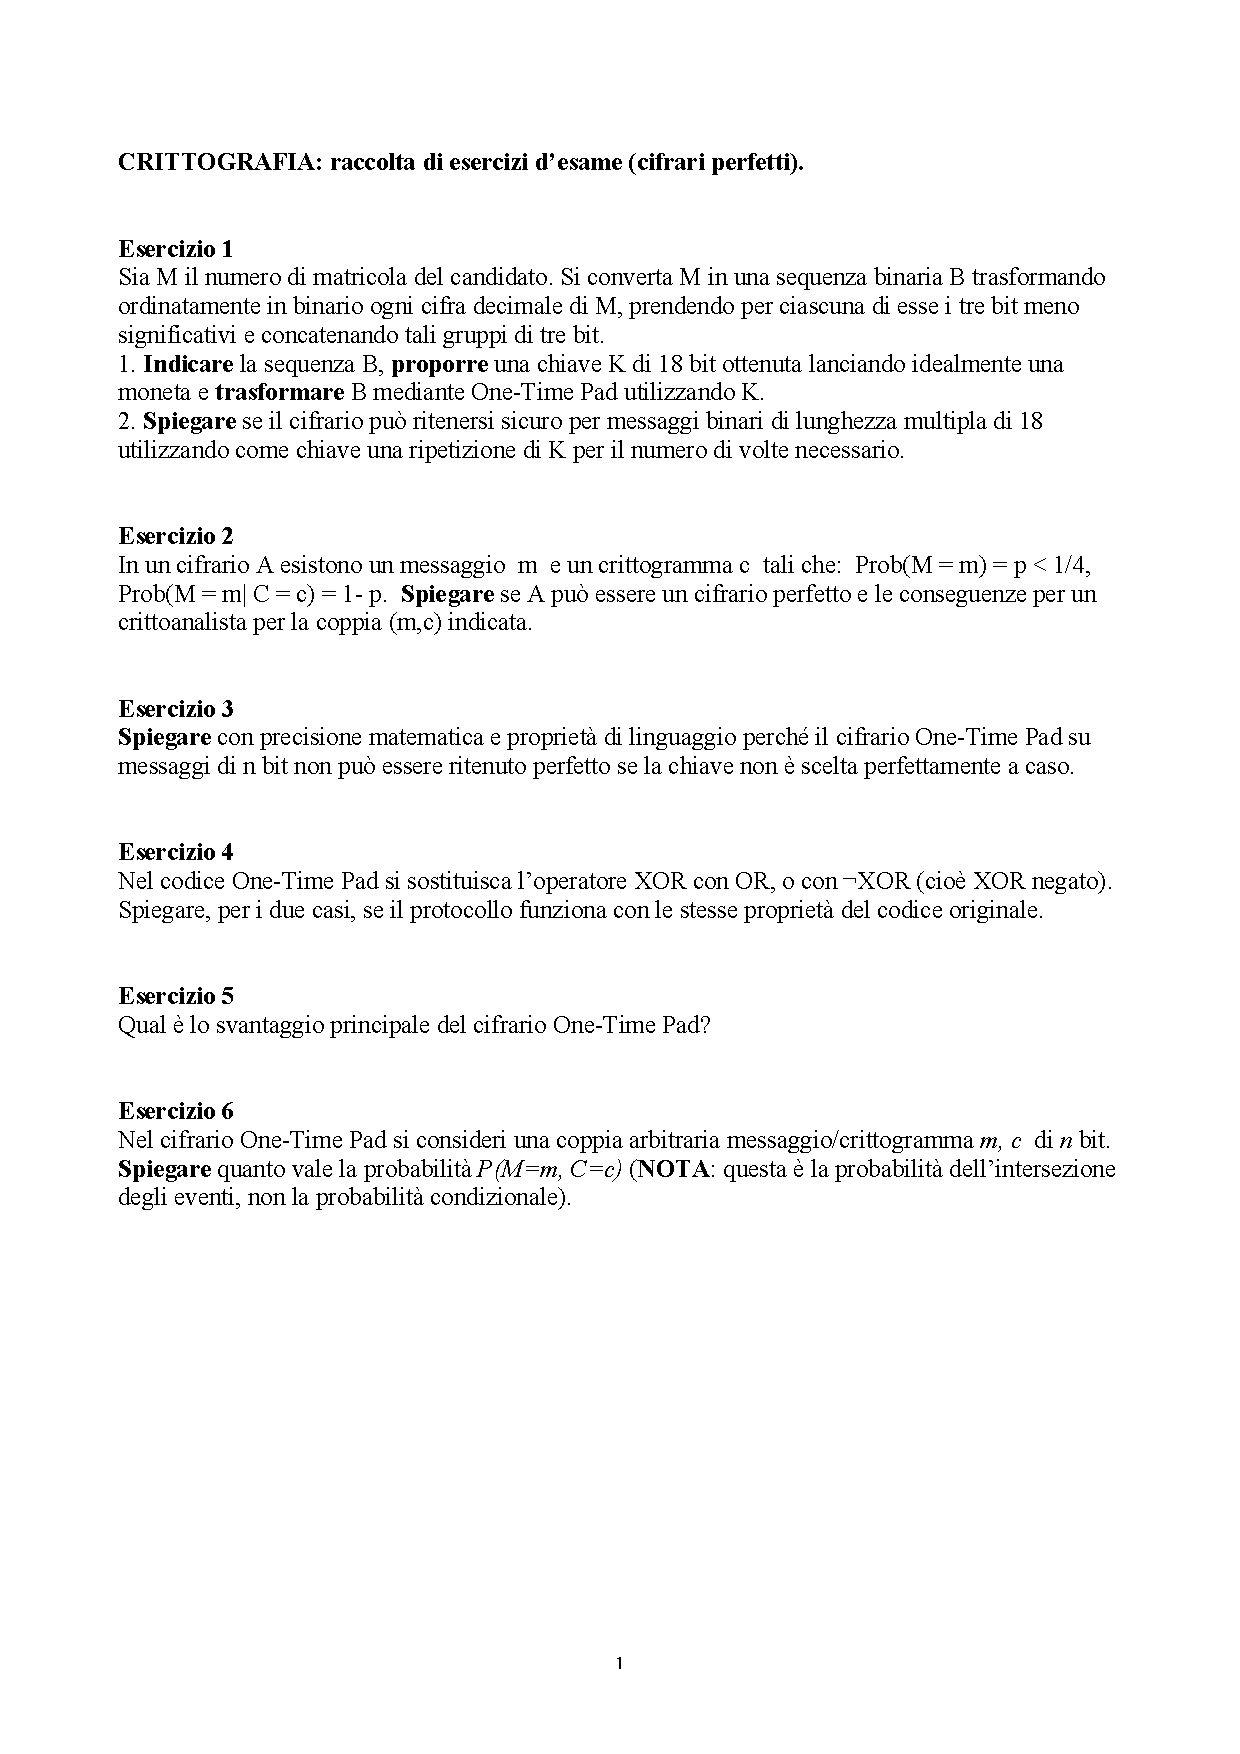
\includegraphics{img/3.PNG}
\end{center}
\paragraph{Esempio 1} $\underbrace{1011}_{\text{B}}|\underbrace{1001}_{9} \Longrightarrow 0xB9$
\paragraph{Esempio 2} $\underbrace{1100}_{\text{C}}|\underbrace{0001}_{1} \Longrightarrow 0xC1$
\section{Osservazione sul calcolo di MB, KB o GB occupati}
Ricordarsi che 
\[\boxed{2^{10}=1\text{ KB}}\,\,\,\,\,\,\,\boxed{2^{20}=1\text{ MB}}\,\,\,\,\,\,\,\boxed{2^{30}=1\text{ GB}}\]
\paragraph{Esempio} Definiamo lo spazio di memoria come l'insieme di $2^{32}$ locazioni.
\[2^{32}=2^{30} \cdot 2^2 = 4\text{ GB}\]
\clearpage
\section{Struttura del calcolatore vista da un programmatore ASS}
Cosa vede un programmatore quando programma un calcolatore? Essenzialmente tre cose: spazio di memoria, spazio di I/0 e processori.
\paragraph{Spazio di memoria}
Con spazio di memoria intendiamo una sequenza lineare e contigua di locazioni: ciascuna di esse ha capacità di un byte ed è identificata da un numero naturale a 32bit detto indirizzo. Se abbiamo $32$ bit significa che potremo esprimere $2^{32}$ indirizzi diversi, quindi avremo $2^{32}$ locazioni possibili (si va da $0x000\dots 00$ a $0x111\dots 11$, se ho $2^{32}$).  Solitamente si accede alla memoria per le seguenti motivazioni:
\begin{itemize}
\item Prelevare istruzioni
\item Prelevare gli operandi delle istruzioni (la maggior parte si trova in memoria, molto spesso nel processore - in particolare nella ALU)
\end{itemize}
può svolgere accessi di lettura o di scrittura, possibili su singola locazione (operando a 8 bit), doppia locazione (operando a 16 bit) e quadrupla locazione (32 bit).
\paragraph{Memoria del computer} La memoria del computer si divide in
\begin{itemize}
\item \textbf{RAM}, \emph{Random Access Memory}. Questa memoria è di tipo volatile, cioè le informazioni vengono mantenute finchè c'è tensione. C'è un problema: cosa fa il processore al momento dell'accensione se l'accesso è appunto casuale? Questo non può succedere e richiede l'introduzione della...
\item \textbf{ROM}, \emph{Read Only Memory}. Memoria di sola lettura, non volatile, che contiene il programma eseguito dal processore al momento dell'accensione.
\end{itemize}
\paragraph{Tipi di accessi} Accessi di tipo diverso, dato lo stesso indirizzo, restituiscono un contenuto diverso. Negli accessi a 16/32bit si utilizza l'indirizzo più piccolo delle 2/4 locazioni. L'indirizzo più grande contiene i bit più significativi, segue quanto presente nell'immagine
\begin{center}
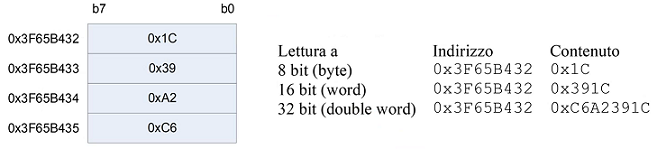
\includegraphics{img/4.PNG}
\end{center}
\paragraph{Dimensione dello spazio di memoria} Che dimensione hanno $2^{32}$ bit? $4$GB di memoria!
%\[\boxed{2^{10} = \text{K}}\;\;\;\;\boxed{2^{20}  = \text{M}}\;\;\;\;\boxed{2^{30}  = \text{G}}\]
Come faccio a sapere se posso riferire un indirizzo (in un calcolatore non sono presente solo io coi miei programmi, c'è anche la ROM, per esempio)? Non è un problema nostro: gli indirizzi in Assembler sono simbolici, ci pensa l'assemblatore a mappare la variabile su una cella utilizzabile.
\paragraph{Spazio di I/0}
Lo spazio di Input/Output consiste in $2^{16}=64$k locazioni (dette anche porte). Ciascuna porta ha una capacità pari ad un byte ed è indirizzabile mediante un indirizzo a 16bit. Possiamo accedere allo spazio di I/O usando due particolari istruzioni (IN e OUT). Contrariamente alle celle dello spazio di memoria le porte di I/0 non sono intercambiabili: a un certo indirizzo abbiamo la tastiera, a un altro il mouse. Segue la necessità di conoscere gli indirizzi! Generalmente
\begin{itemize}
\item si eseguono istruzioni IN per prelevare uno o più byte da un dispositivo: dati da elaborare o semplicemente informazioni sullo stato del dispositivo.
\item si eseguono istruzioni OUT per trasmettere uno o più byte a un dispositivo: dati elaborati o informazioni per modificare lo stato del dispositivo.
\end{itemize}
\paragraph{Processore} Il processore consiste in una collezione di registri. Un registro consiste in una piccola locazione di memoria, avente 32 bit. Si hanno due tipi di registri:
\begin{itemize}
\item \textbf{Registri generali}. Si osserva che tutti i registri sono introdotti dalla lettera E: questa sta per \emph{Extended}. Precedentemente un registro occupava solo 16bit, successivamente sono stati estesi a 32 bit. La $E$ risolve anche questioni non banali di compatibilità: è possibile richiamare l'intero registro con i suoi 32 bit col nome $EXY$, ma possiamo riferire la parte bassa dei registri col nome vecchio ($XY$)!
\begin{center}
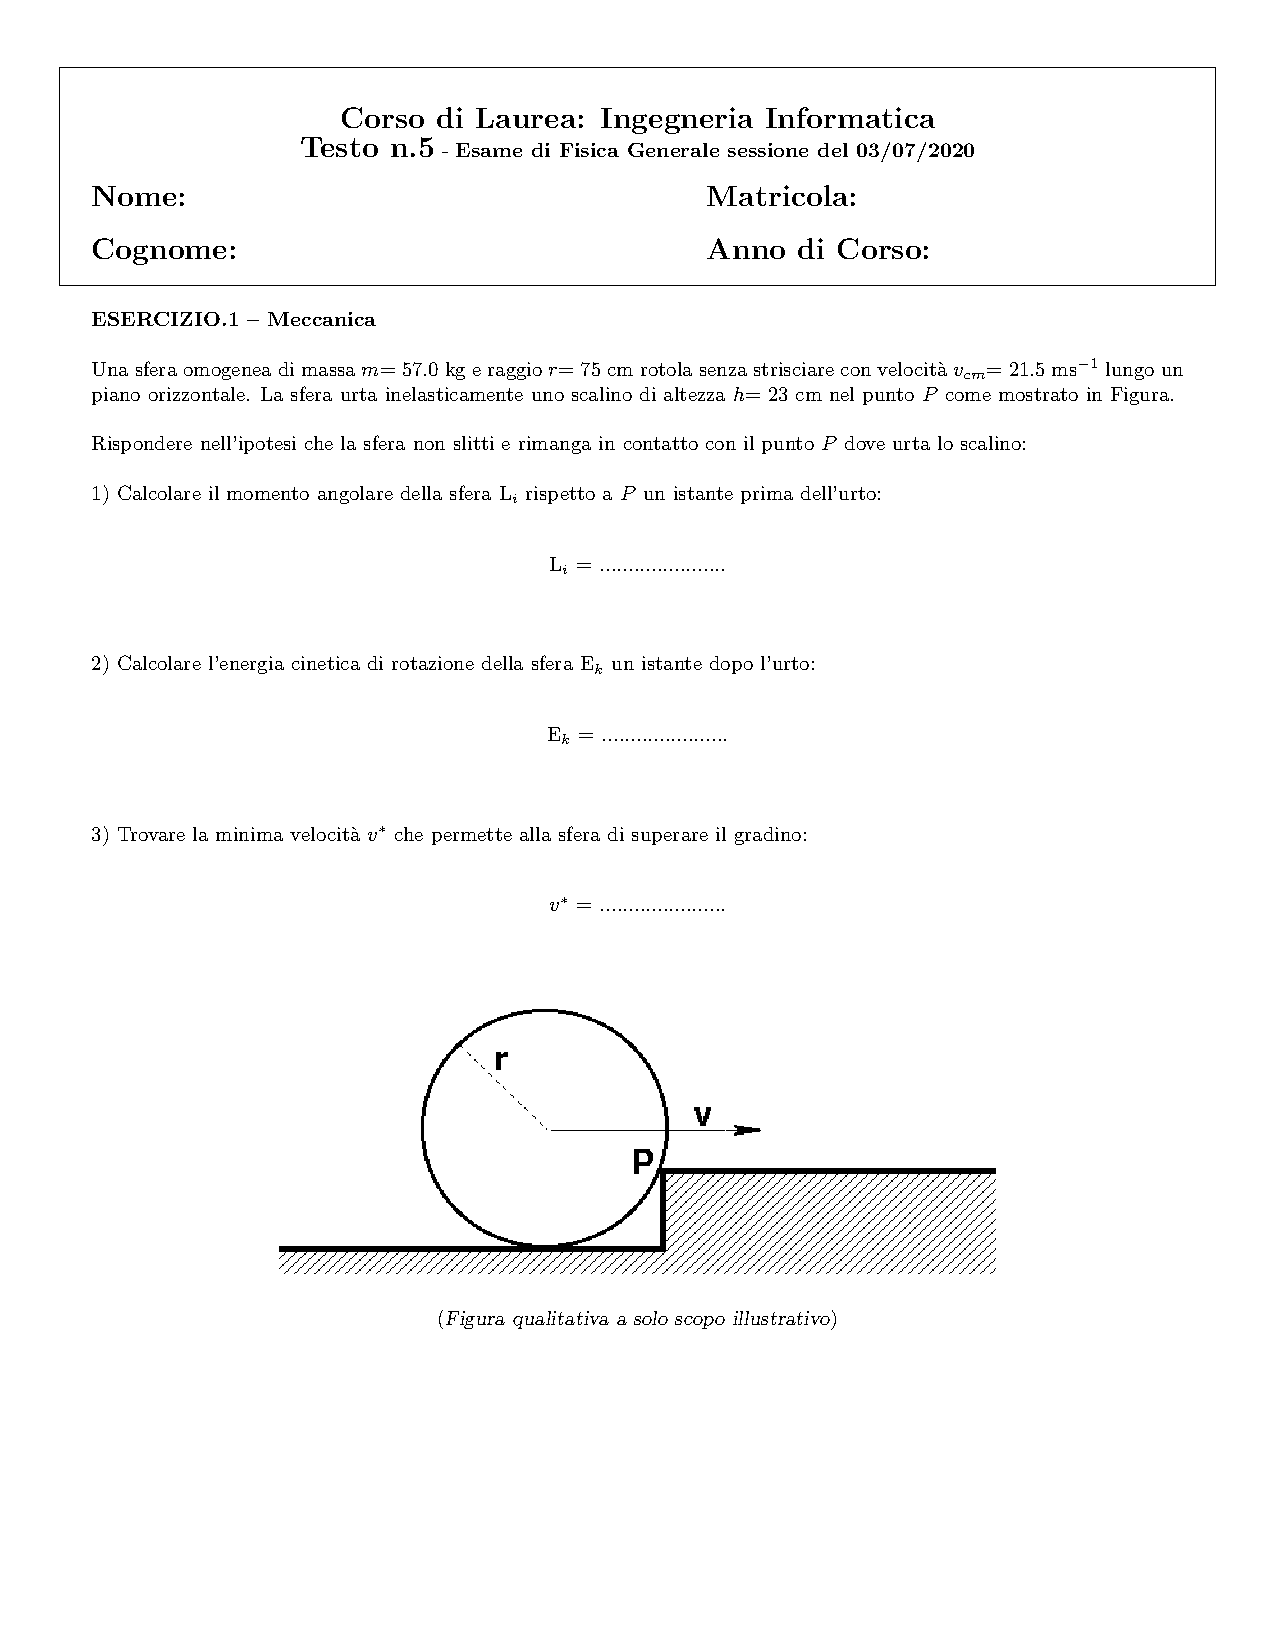
\includegraphics{img/5.PNG}
\end{center}
Risulta possibile richiamare la prima parte bassa e la seconda parte bassa con $XH$ ed $YL$, dove $H$ sta per \emph{High} ed $L$ sta per \emph{Low}.\\\\
I nomi dei registri sono i seguenti:
\begin{center}
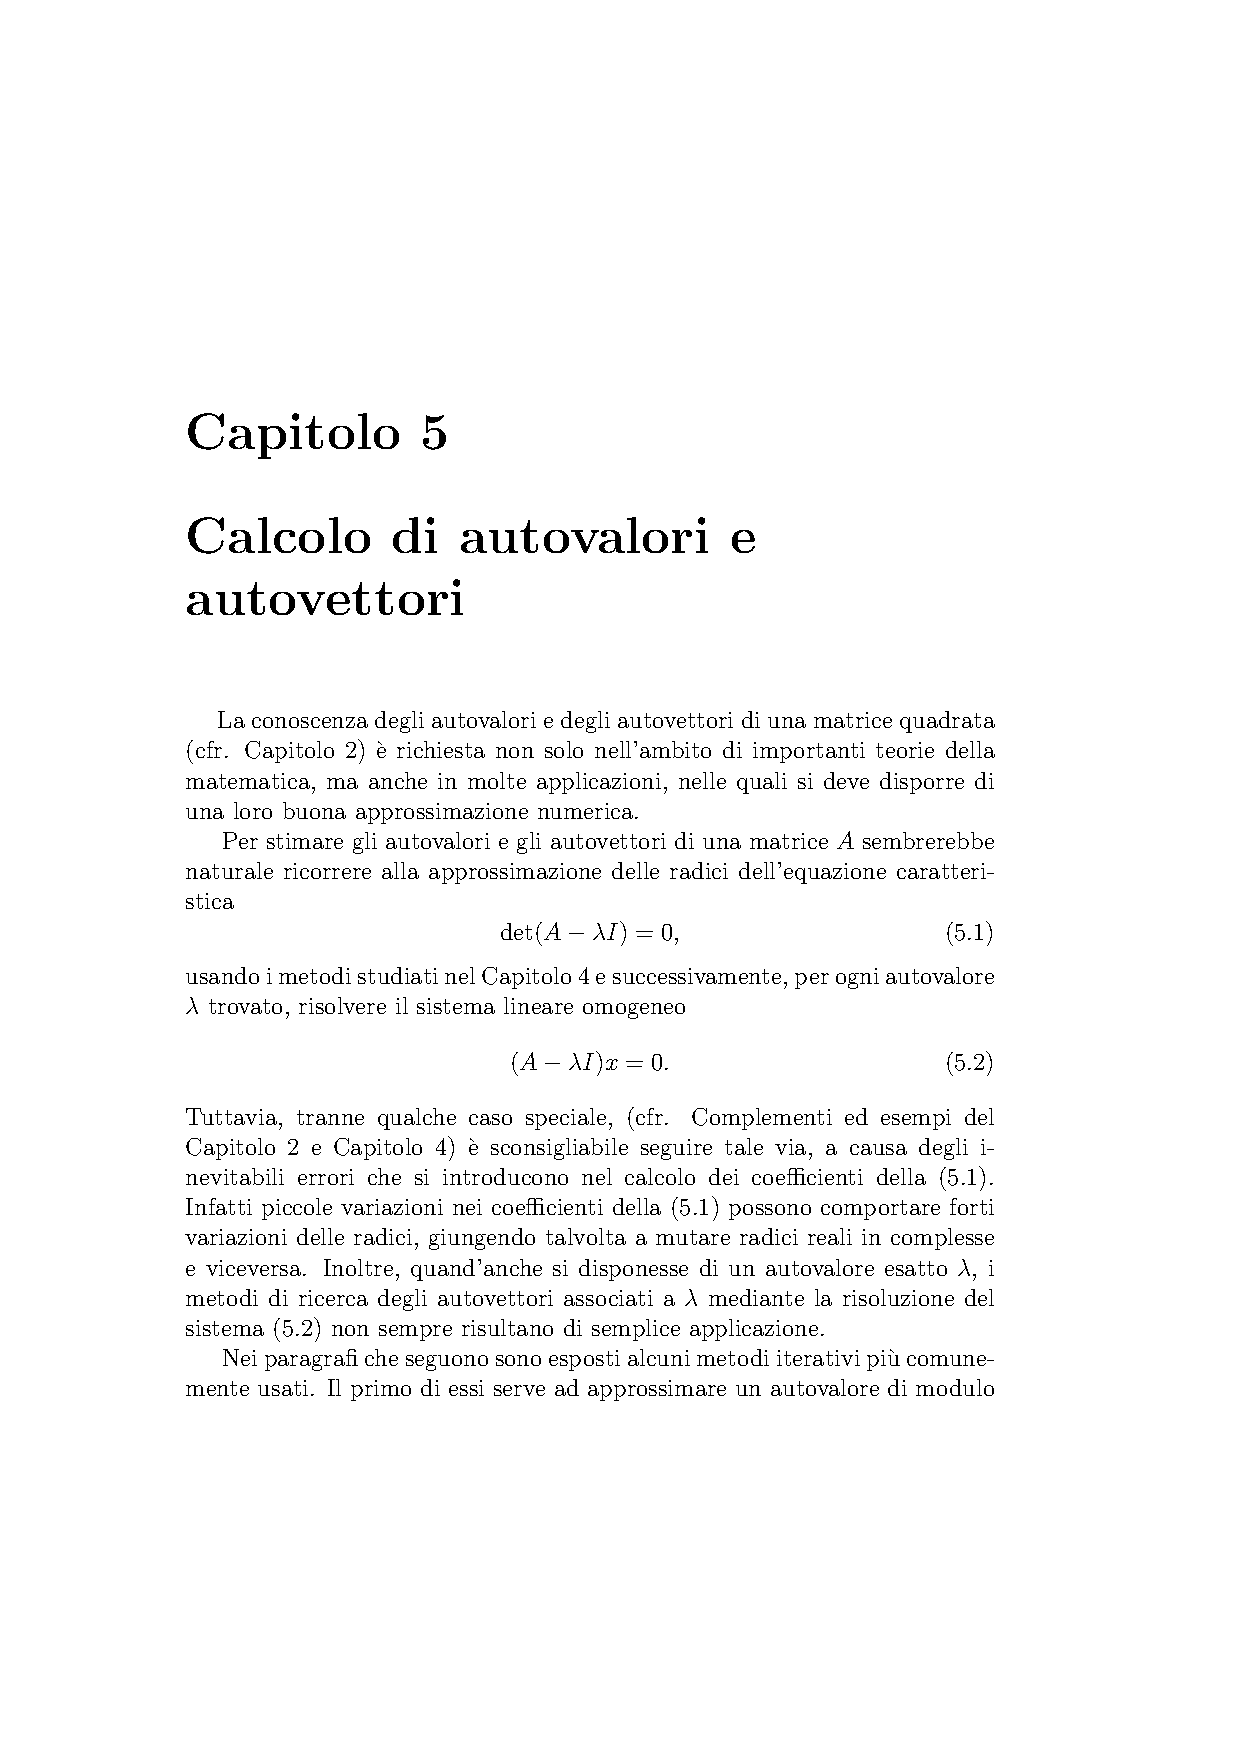
\includegraphics{img/6.PNG}
\end{center}
Alcuni  di questi sono utilizzati per particolari funzioni:
\begin{itemize}
\item EAX è detto registro accumulatore ed è usato da alcune istruzioni aritmetiche (per esempio per variabili incremento)
\item ESI, EDI, EBX ed EBP sono detti registri puntatore, dove $B$ sta per \emph{base} ed $I$ sta per \emph{indice}.
\item ESP, utilizzato per indirizzare la pila. Solitamente si utilizza per gestire sottoprogrammi
\end{itemize}
Per comprendere l'utilità di alcuni registri leggere sull'\emph{indirizzamento di memoria}.
\item \textbf{Registri di stato}. I registri di stato sono due:
\begin{itemize}
\item EIP, cioè \emph{Instruction Pointer register} (detto anche \emph{program counter}). Consiste nel registro contenente la locazione di memoria a partire dalla quale sarà prelevata la prossima istruzione. Il suo contenuto è fissato al momento dell'accensione del processore! Raffiniamo quanto detto all'inizio: il processore
\begin{enumerate}
\item preleva dalla memoria, precisamente all'indirizzo EIP, la nuova istruzione
\item incrementa EIP del numero di byte dell'istruzione che ha prelevato (si parla di istruzioni contigue, ovviamente la cosa cambia se si incontrano salti)
\item esegue l'istruzione e ritorna allo step (1)
\end{enumerate}
\underline{EIP inizialmente vale $0xFFFF0000$: la prima istruzione si trova lì}. Ovviamente le celle successive dovranno essere implementate in ROM.\\

\item EF, cioè \emph{Extended Flag register}. Il registro consiste in 32 elementi detti \emph{flag}. Ci interessano, in particolare, i seguenti flag:
\begin{itemize}
\item OF (Overflow): elemento impostato ad $1$ quando il risultato generato dall'ultima istruzione \emph{trabocca}
\item SF (Sign): elemento impostato ad $1$ quando il risultato generato dall'ultima istruzione restituisce un qualcosa con $MSB=1$
\item ZF (Zero): elemento impostato ad $1$ quando il risultato generato dall'ultima istruzione restituisce un qualcosa con tutti bit nulli
\item CF (Carry): elemento impostato ad $1$ quando il risultato generato dall'ultima istruzione genera un riporto o un prestito.
\end{itemize}
Per gli interi ci serviranno OF, SF, ZF (CF è inutile), per i naturali CF e ZF (OF ed SF sono inutili). \underline{Nel registro dei flag quelli che ci interessano valgono $0$, inizialmente}.
\end{itemize}
\end{itemize}

\chapter{Mercoledì 30/09/2020}
\section{Codifica macchina e codifica mnemonica}
Presente a pagina 7 della dispensa di Assembler.
\section{Struttura di un'istruzione}
Le istruzioni sono formate da tre campi:
\begin{itemize}
\item Il \textbf{codice operativo}, il nome dell'istruzione che vogliamo eseguire
\item Il \textbf{suffisso di lunghezza} (lunghezza degli operandi): sono ammesse come lunghezze B (byte, 8it), W (word, 16bit), L (long, 32bit). Non dobbiamo porre il suffisso obbligatoriamente: ci pensa l'assemblatore se la lunghezza degli operandi può essere intuita (per esempio quando almeno uno degli operandi è un registro).
\item \textbf{Operandi}: le istruzioni ammettono 0/2 operandi (sono poche le istruzioni con 0 operandi). Nelle istruzioni con due operandi si distingue l'operando \textbf{sorgente} dall'operando \textbf{destinatario}. Se si ha un solo operando quello è detto \textbf{source} (destinatario è implicito) o \textbf{destinatario} (se l'istruzione lavora con un solo operando e pone nell'operando stesso il risultato del suo lavoro). I due operandi (salvo rare eccezioni) hanno la stessa lunghezza! Gli operandi possono essere in registri o porte I/O, ma possono essere anche costanti!
\end{itemize}
Un esempio di istruzione è la seguente
\begin{verbatim}
ADD %BX, pippo
\end{verbatim}
il contenuto presente all'indirizzo di una locazione di memoria (\emph{pippo}) viene incrementato del valore contenuto nella libreria BX. 
Il linguaggio Assembler consente al programmatore di riferire le locazioni di memoria con nomi simbolici che l'assemblatore tradurrà in indirizzi. L'assemblatore \underline{si incaricherà di sostituire lo stesso indirizzo tutte le volte che trova scritto \emph{pippo}}.

\section{Esempio di programma}
Presente un esempio di programma, accompagnato da spiegazione, da pagina 8 a pagina 11 della dispensa di Assembler.

\section{Memoria occupata da una certa istruzione}
Sia sul libro di Corsini che sulla dispensa di Stea si definisce un'istruzione come una stringa che occupa da 1 a 14 byte. Tenendo conto delle cose appena introdotte osserviamo che
\begin{itemize}
\item Il numero di operandi è uno degli indicatori dello spazio occupato da una certa istruzione (è ovvio che un'istruzione senza operandi possa occupare meno di un'istruzione con un operando, stessa cosa se mettiamo a confronto istruzioni con uno e due operandi, rispettivamente)
\item Lo spazio occupato dagli operandi dipende dall'indirizzamento adottato: nel caso di indirizzamento diretto abbiamo una costante; in tutti gli altri casi andiamo a salvare l'indirizzo dell'area di memoria in cui si trova un certo operando.
\item Ricordiamo che un processore, nell'ordine:
\begin{itemize}
\item estrae da EIP l'indirizzo dell'istruzione successiva
\item incrementa EIP in modo tale che questa punti alla nuova istruzione successiva
\item esegue l'istruzione estratta poco fa ed eventualmente preleva dalla memoria gli operandi necessari per eseguire l'istruzione (usando gli indirizzi salvati)
\end{itemize}
\item Ricordarsi le dimensioni di un'istruzione: sono allocati al più 4byte per Displacement! Segue che non è possibile, in un'istruzione a due operandi, fare indirizzamenti di memoria in entrambi gli operandi.
\end{itemize}
\section{Indirizzamento degli operandi}
Ricordiamo la struttura di un'istruzione
\begin{verbatim}
OPCODEsize source, destination
\end{verbatim}
\subsection{Indirizzamento di registro}
L'indirizzamento \textbf{NON} è possibile con i registri di stato. Possiamo scegliere tra i seguenti registri generali:
\begin{itemize}
\item 8 registri a 32bit (EAX, EBX, ECX, EDX, EBP, ESI, EDI, ESP)
\item 8 registri a 16 bit (AX, BX, CX, DX, SI, DI, SP , BP)
\item 8 registri ad 8 bit (AH, BH, CH, DH, AL, BL , CL, DL)
\end{itemize}
operandi di registro possono essere sia sorgente che destinatario
\begin{verbatim}
OPCODE %DI
OPCODE %EAX, %EBX
OPCODE %AH, %CL
\end{verbatim}
la prima istruzione lavora su un operando a 16bit, la seconda su operandi a 32bit, la terza su operandi ad 8 bit. Noi non sappiamo quali sono le istruzioni (e quindi la dimensione che occuperanno queste istruzioni), ma sappiamo già che potremo omettere il suffisso di dimensione (grazie alla presenza di almeno un operando con indirizzamento di registro).

\subsection{Indirizzamento immediato}
Questo tipo di indirizzamento può essere usato solo nell'operando sorgente: scriviamo una costante direttamente nell'istruzione (per ovvie ragioni non ha senso porre una costante nel destinatario).
\begin{verbatim}
OPCODE $0x20, %AL
OPCODE $0x5683a20b, %ECX
\end{verbatim}
nella prima lavoro su operandi ad 8 bit, nella seconda su operandi a 32bit.

\subsection{Indirizzamento di memoria}
L'indirizzamento di memoria è complicato, ma fondamentale: il processore, per la maggior parte del tempo, copia pezzi di memoria da una parte a un'altra. L'indirizzamento di memoria è possibile sia con l'operando sorgente che con quello destinatario, ma non è possibile farlo in entrambi in una stessa istruzione (l'assemblatore da errore se ci proviamo). 
\paragraph{Caso più generale} Il caso più generico di indirizzo è il seguente
\[\text{Indirizzo}=\left|\text{base}+\text{indice}\times\text{scala} \pm \text{displacement}\right|_{\text{modulo}_{2^{32}}}\]
cioè 
\begin{verbatim}
OPCODEsfx +-disp(base,indice,scala)
\end{verbatim}
\begin{itemize}
\item la base e l'indice consistono in registri generali a 32 bit. Precedentemente era obbligatorio porre un registro B in base e un registro I in indice: oggi si offre maggiore flessibilità e si possono utilizzare tutti i registri generali.
\item scala è una costante che può avere per valore $1$ (valore default se non indicato), $2,4,8$.
\item displacement è una costante intera. 
\end{itemize}
\subsubsection{Indirizzamento di tipo diretto}
Nelle cose viste fino ad ora abbiamo fatto indirizzamenti di memoria diretti, cioè indirizzamenti con solo il displacement.
\begin{verbatim}
OPCODEW 0x00002001
\end{verbatim}
\subsubsection{Indirizzamento di tipo indiretto}
Specifico un solo registro, precisamente un registro puntatore. 
\paragraph{Registro base} Poniamo la cosa nella seguente forma
\begin{verbatim}
OPCODEL (%EBX)
\end{verbatim}
dove EBX consiste nel registro contenente l'indirizzo. Attenzione: è necessario indicare il suffisso di lunghezza, non abbiamo un indirizzamento di registri.
\paragraph{Registro indice} Se volessi indicare un registro indice pongo
\begin{verbatim}
OPCODEL (,%ESI, 4)
\end{verbatim}
la scala moltiplica solo l'indice e non la base.

\subsubsection{Indirizzamento con displacement e registro di modifica}
\begin{verbatim}
OPCODEW 0x002A3A2B (%EDI)
\end{verbatim}
Indirizzo un operando a 16bit, che si trova nella doppia locazione il cui indirizzo si ottiene sommando (modulo $2^{32}$) il displacement e il contenuto di EDI. Questa cosa è molto versatile per i vettori
\subsubsection{Indirizzamento bimodificato senza displacement}
\begin{verbatim}
OPCODEW (%EBX, %EDI)
OPCODEW (%EBX, %EDI, 8)
\end{verbatim}
utilizzo due registri puntatori ponendo, eventualmente, la scala.

\subsubsection{Indirizzamento bimodificato con displacement}
In questo caso utilizzeremo tutte le armi a nostra disposizione
\begin{verbatim}
OPCODEB 0x002F9000 (%EBX, %EDI)
OPCODEB -0x9000 (%EBX, %EDI)
\end{verbatim}

\subsection{Indirizzamento delle porte di I/O}
L'indirizzo di I/O può avvenire sia con la sorgente che col destinatario, ma mai con entrambi. L'indirizzamento può essere diretto o indiretto con registro puntatore
\begin{itemize}
\item Possibili porre solo indirizzi su 8bit nell'indirizzamento diretto (perchè la macchina fornisce solo 8bit)
\item L'indirizzamento indiretto è possibile solo usando il registro DX
\end{itemize}
Vediamo i seguenti esempi
\begin{verbatim}
IN 0x001A, %AL
IN (%DX), %AX
OUT %AL, 0x003A
OUT %AL, (%DX)
\end{verbatim}
La prima istruzione preleva un operando a 8bit dalla porta di I/0 0x001A e pone il contenuto presente a quell'indirizzo nel registro AL, la terza pone il contenuto del registro Al nella porta di I/0 avente indirizzo 0x003A.
\clearpage
\section{Principali istruzioni}
Si distinguono 
\begin{itemize}
\item Istruzioni operative
\begin{multicols}{2}\begin{itemize}
\item Istruzioni di trasferimento
\item Istruzioni aritmetiche
\item Istruzioni di traslazione/rotazione
\item Istruzioni logiche
\end{itemize}
\end{multicols}
\item Istruzioni di controllo
\begin{itemize}
\item Istruzioni di salto
\item Istruzioni per la gestione di sottoprogrammi
\end{itemize}
\end{itemize}
Per ogni istruzione diremo:
\begin{itemize}
\item il formato
\item cosa fa
\item se ci sono aggiornamenti di flag
\item le modalità di indirizzamento ammesse per gli operandi
\end{itemize}
le istruzioni sono spiegate in modo dettagliato nella bibbia di Corsini.
\subsection{Istruzioni di trasferimento}
Ribadiamo che gli spostamenti possibili sono i seguenti
\[\boxed{\text{Memoria} \longleftrightarrow \text{Registro}}\;\;\;\;\boxed{\text{Registro} \longrightarrow \text{Registro}}\;\;\;\;\boxed{\text{I/0} \longleftrightarrow \text{Registro}}\]
non è possibile fare trasferimenti da memoria a memoria. Le istruzione di trasferimento, inoltre, non modificano i flag.
\subsubsection{MOVE}
\begin{center}
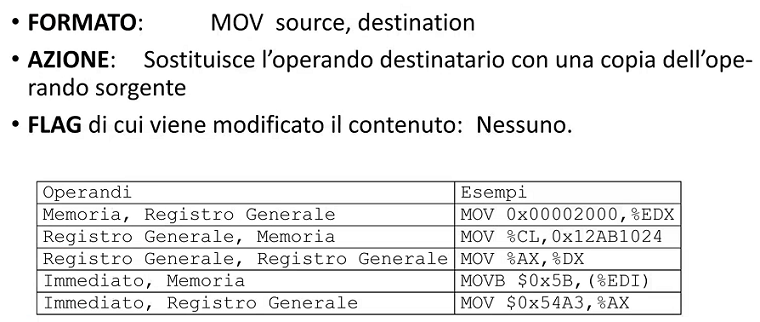
\includegraphics{img/7.PNG}
\end{center}
\subsubsection{LOAD EFFECTIVE ADDRESS}
\begin{center}
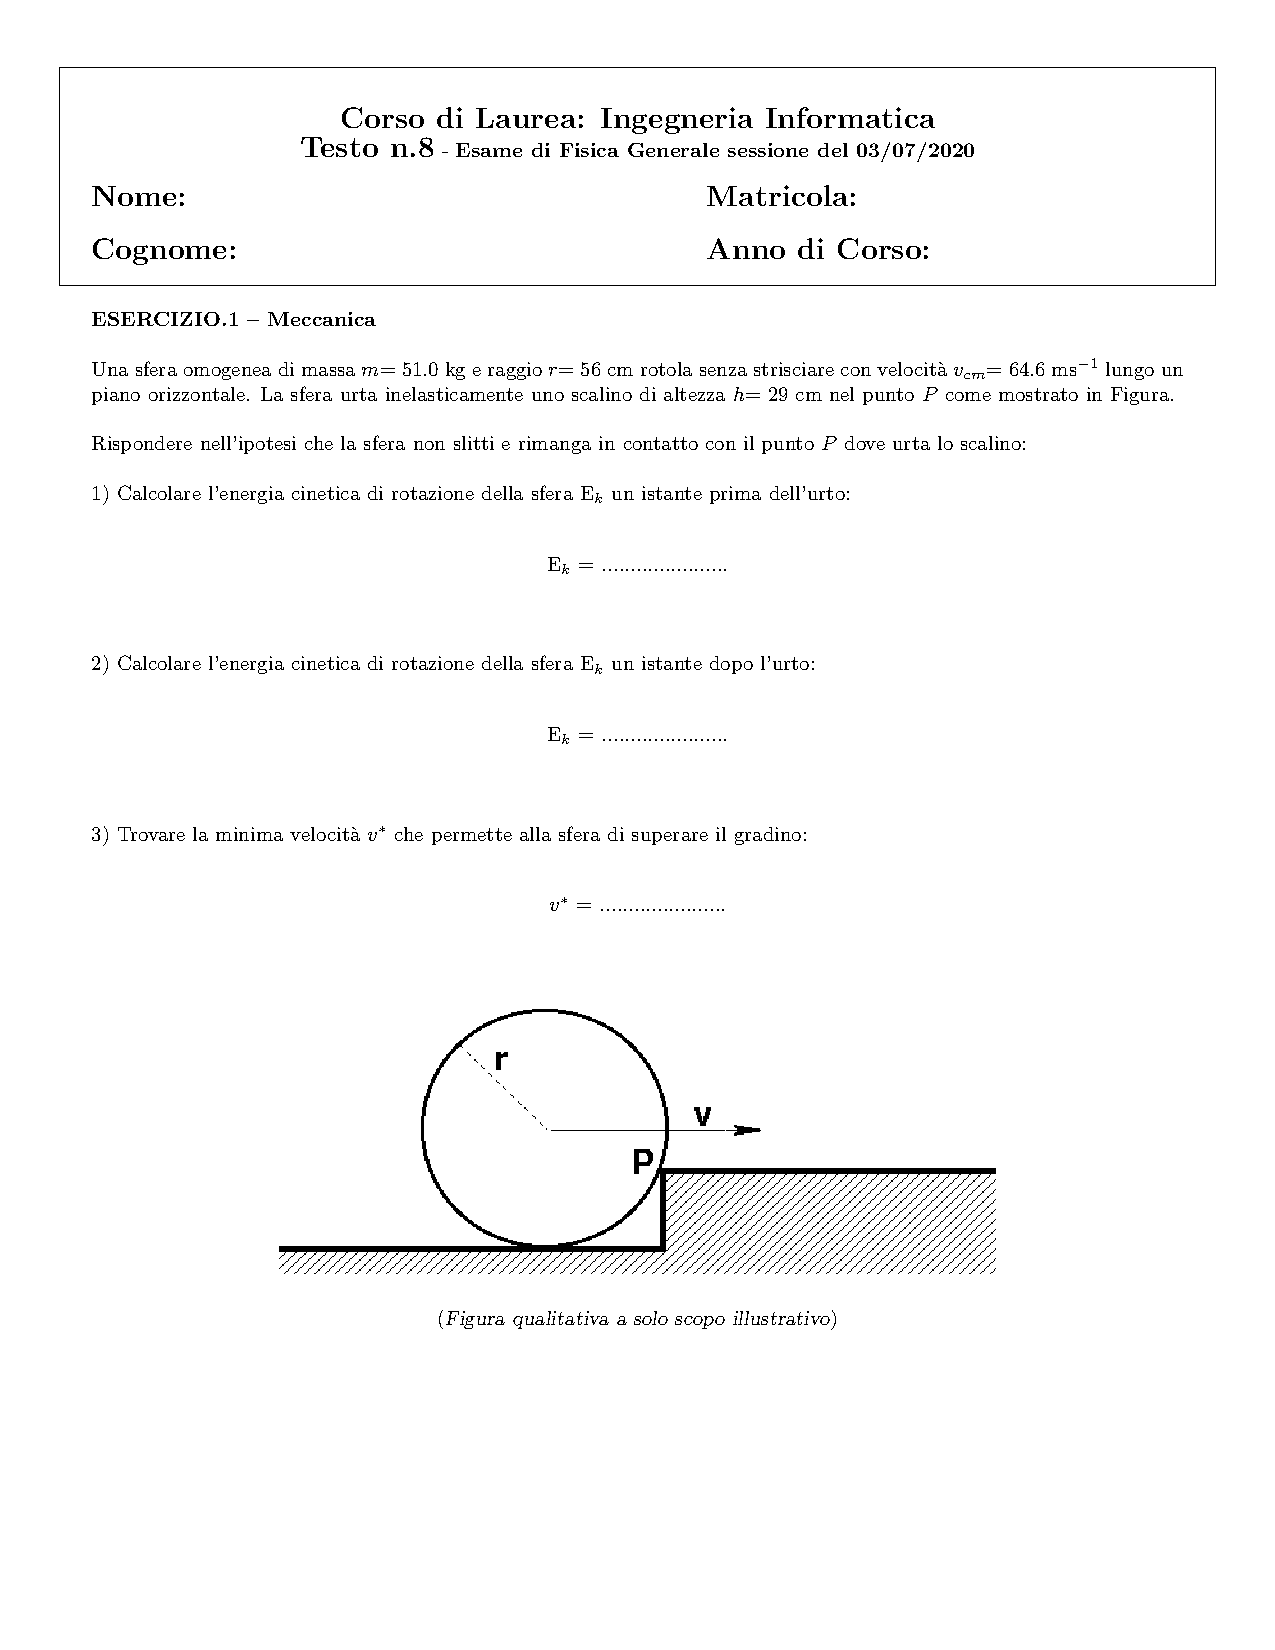
\includegraphics{img/8.PNG}
\end{center}
Col primo esempio intendiamo \emph{copia l'indirizzo 0x00002000 nel registro EDX}. col secondo intendiamo \emph{copia il risultato dell'operazione di indirizzamento di memoria nel registro ECX}. 
\paragraph{Differenza tra MOV e LEA} La MOV copia il contenuto posto a quell'indirizzo, la LEA copia l'indirizzo!

\subsubsection{EXCHANGE}
\begin{center}

\includegraphics{img/9.PNG}
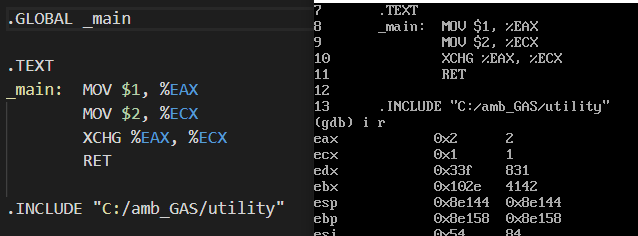
\includegraphics{img/215.PNG}
\end{center}

\chapter{Giovedì 01/10/2020}
\section{Concludiamo con le istruzioni di trasferimento}
\subsection{INPUT e OUTPUT}
\begin{center}

\includegraphics{img/12.PNG}

\includegraphics{img/13.PNG}
\end{center}
Gli operandi nell'I/O si possono trasferire solo nei/dai registri generali. Non si fanno operazioni sulle porte! Inoltre, gli unici registri utilizzabili sono AL, AX (come sorgente o destinatario) e DX (come registro puntatore). 
\subsubsection{ASSEMBLER non è linguaggio ortogonale}
Contrariamente al C++ Assembler non può essere definito un linguaggio ortogonale (in C++ posso mettere qualunque variabile se la sintassi mi consente di scrivere una variabile). Cose che sono fatte con un certo registro generale non è detto possano essere fatte con altri registri. 
\subsubsection{Uscita da registro a porta}
Supponiamo di voler passare il contenuto del registro BX (si possono effettuare trasferimenti solo dai registri AL e AX) alla porta con indirizzo 0x3142. Scriveremo le seguenti istruzioni
\begin{verbatim}
MOV %BX, %AX
MOV $0x3142, %DX
MOV %AX, (%DX)
\end{verbatim}
ricordiamo che non è possibile fare trasferimenti da memoria a memoria. Inoltre, nei formati dove la sorgente (input) o il destinatario (output) sono indirizzi è necessario che l'indirizzo sia inferiore a 256.

\subsection{Pila}
Abbiamo già visto la pila a Fondamenti di programmazione: una struttura dati dove il contenuto è gestito secondo la regola LIFO (\emph{Last in First Out}, cioè l'ultimo elemento inserito è il primo ad andarsene). Al di là della questione C++, la pila è essenziale per il funzionamento del calcolatore, precisament per annidare sottoprogrammi (L'assembler stesso è organizzato per sottoprogrammi)
\begin{itemize}
\item Quando avvio un sottoprogramma salvo l'indirizzo di ritorno, cioè quello dell'istruzione successiva e lo pongo nella pila (\emph{push})
\item Quando termino l'esecuzione del sottoprogramma faccio \emph{pop}, cioè estraggo dalla pila l'ultimo indirizzo inserito (quello della prossima istruzione da eseguire).
\end{itemize}
La pila permette di chiamare sottoprogrammi all'interno di altri sottoprogrammi.
\paragraph{Puntatore al top della pila} Il registro ESP (\emph{Extended stackpointer}) mi permette di puntare all'elemento più alto della pila. 
\paragraph{\emph{push} value} Decremento ESP in modo tale che punti alla zona di memoria immediatamente superiore, copio un certo valore in \%ESP
\paragraph{\emph{push} dest} Copio il contenuto di \%ESP nel destinatario e incremento ESP in modo tale da puntare alla zonna di memoria immediatamente inferiore.
\paragraph{ESP deve essere inizializzato} Ogni programma che utilizza la pila deve inizializzare ESP assegnando un valore sensato.
\begin{center}

\includegraphics{img/14.PNG}
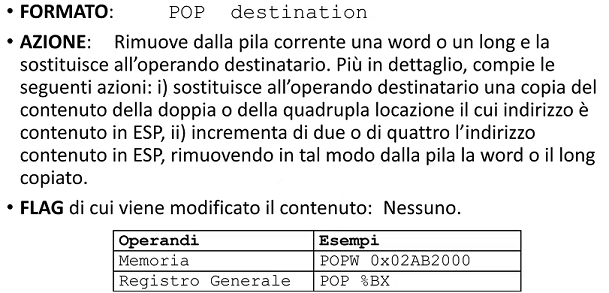
\includegraphics{img/15.PNG}
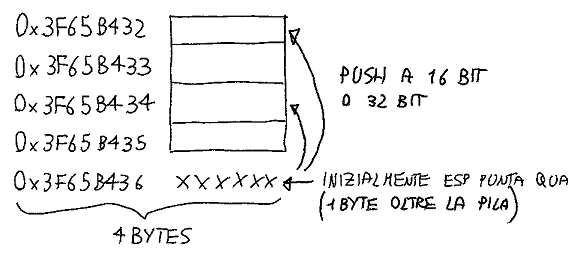
\includegraphics{img/212.PNG}
\end{center}
Gli operandi salvati ed ottenuti dalla pila devono essere a 16 o a 32 bit. Se non si ha un registro generale come operando è necessario indicare il suffisso di lunghezza (per forza W o L, come già detto).

\subsubsection{Pila come memoria temporanea}
La pila può essere usata come \emph{parcheggio di dati}. I registri generali sono pochi e in alcune istruzioni sono gli unici operandi possibili. In alcune circostanze, addirittura, potrei essere costretto a usare lo stesso registro per due scopi diversi in momenti diversi (e se volessi recuperare il dato trovato nel primo momento?). 
\paragraph{Esempio banalissimo della POP} Osserviamo il valore di EAX dopo aver eseguito la POP:
\begin{center}
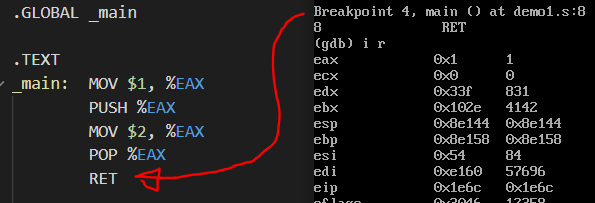
\includegraphics{img/216.PNG}
\end{center}
Il valore di EAX, dopo la PUSH, è $2$. Con la POP recupero il valore impostato precedentemente.

\subsection{PUSHAD e POPAD}
\paragraph{Significato} Per il prof $A$ dovrebbe stare per ALL e $D$ per double. Non è sicuro.
\begin{center}
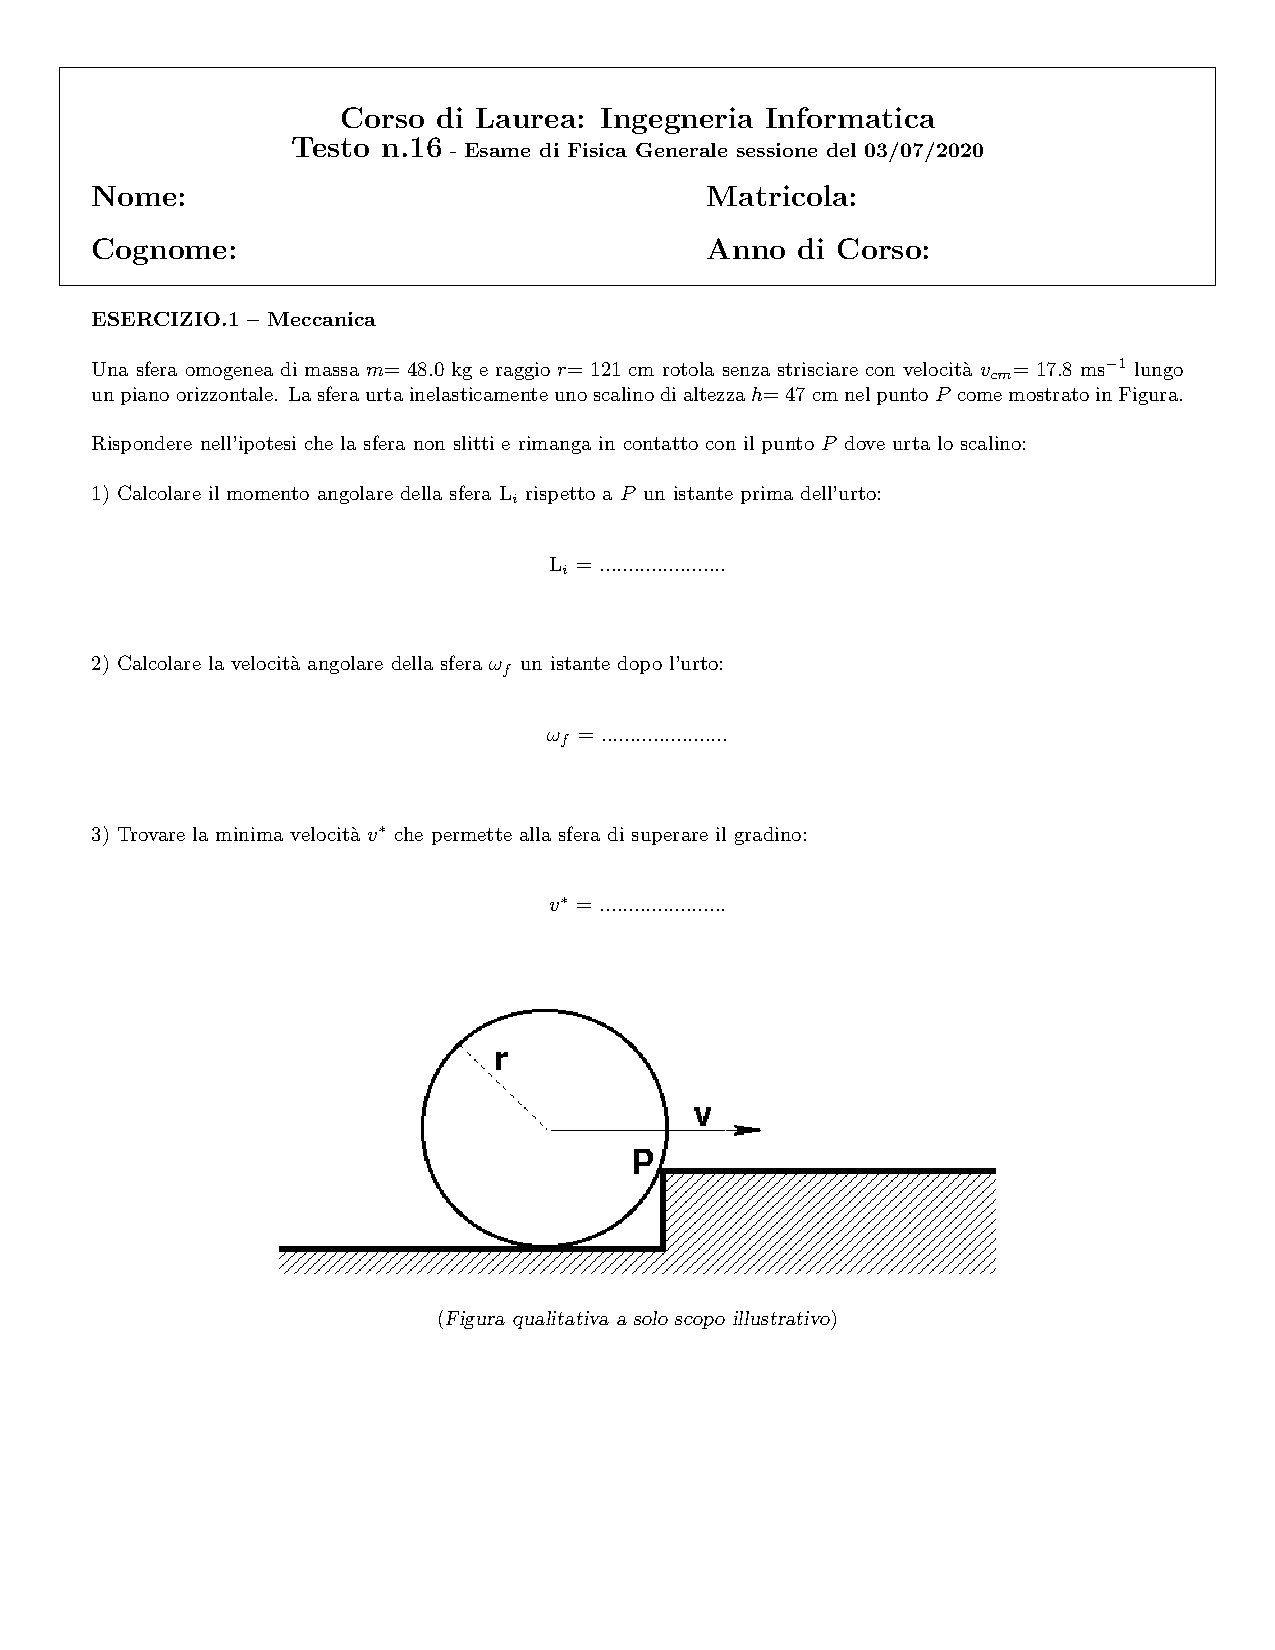
\includegraphics{img/16.PNG}
\end{center}
Chiaramente l'ESP verrà modificato non perchè poniamo noi un valore, ma perchè eseguiamo l'operazione POP (quindi L'ESP sarà incrementato quanto necessario).

\section{Istruzioni aritmetiche}
Introduzione a pagina 13 sulle dispensa di Assembler
\subsection{ADD e SUBTRACT}
Spiegazioni con algoritmo e flag coinvolte da pagina 13 a pagina 17 della dispensa di Assembler.
\[\boxed{\text{dest} \,+\,= \text{src}}\;\;\;\;\boxed{\text{dest}\, -= \,\text{src}}\]
\paragraph{Osservazioni} 
\begin{itemize}
\item Gli algoritmi, sia per l'addizione che per la sottrazione, sono gli stessi sia nei naturali che negli interi (ovviamente negli interi solo con rappresentazione in complemento a 2.
\item Le proprietà tipiche della rappresentazione in C2 (spiegate nella parte relativa all'aritmetica) chiariscono perchè si possa utilizzare la stessa circuiteria, quindi svolgere le operazioni su naturali e interi utilizzando la stessa istruzione.
\item La differenza tra lo svolgere operazioni su interi o naturali sta nei flag da osservare: la circuiteria modifica, in qualunque caso, tutti i flag relativi. Solo NOI sappiamo se quel numero è naturale o intero, segue che siamo noi (con le operazioni successive) a scegliere quali flag leggere (e quindi se trattare il risultato come un intero o un naturale).
\item Precisamente:
\begin{itemize}
\item Nei naturali controlliamo i flag CF, SF e ZF. In particolare se $\text{CF}=1$ significa che l'ultimo riporto da una cifra in più al risultato finale, quindi siamo usciti dall'intervallo di rappresentazione.
\item Negli interi controlliamo i flag OF, SF e ZF. Il CF può avere valore uguale ad $1$ come prima, ma non è più indicatore della validità del risultato. Andremo a vedere la Overflow flag, che
\begin{itemize}
\item è uguale ad $1$ se nell'addizione si è avuto riporto con operandi di segno concorde.
\item è uguale a $0$ se gli operandi dell'addizione sono di segno discorde (il riporto si ignora)
\item è uguale ad $1$ se nella sottrazione si è avuto prestito con operandi di segno discorde
\item è uguale a $0$ se gli operandi della sottrazione sono di segno concorde (il prestito si ignora)
\end{itemize}
\end{itemize}
\item In caso di Overflow negli interi il MSB indicherà un segno sbagliato.
\end{itemize}
Relativamente alla sottrazione se scriviamo l'operazione possiamo ricondurci ai casi dell'addizione (somma di elementi concordi, non sempre rappresentabile, o somma di elementi discordi, sempre rappresentabile).
\subsection{INCREMENT e DECREMENT}
Queste due istruzioni esistono per ragioni soprattutto storiche: molti anni fa la circuiteria più lenta era quella che svolgeva somme e sottrazioni. Avere una funzione di incremento e decremento permetteva di rendere più veloci certe operazioni. Oggi non è più la stessa cosa parlare di costi di operazione: i processori, in molte situazioni, eseguono operazioni in parallelo.
\begin{center}

\includegraphics{img/10.PNG}

\includegraphics{img/11.PNG}
\end{center}
\paragraph{Osservazione} La increment e la decrement non modificano il CF. Questa cosa è evidente nell'esercizio a pagg.32-33 della dispensa di Assembler (programma che permette di verificare se la stringa di bit è palindroma). Nel ciclo viene utilizzata la decrement: se questa modificasse il CF ci sarebbero problemi.

\subsection{ADD WITH CARRY e SUBTRACT WITH BORROW}
Informazioni presenti a pagina 65 e 66 della dispensa di Assembler.

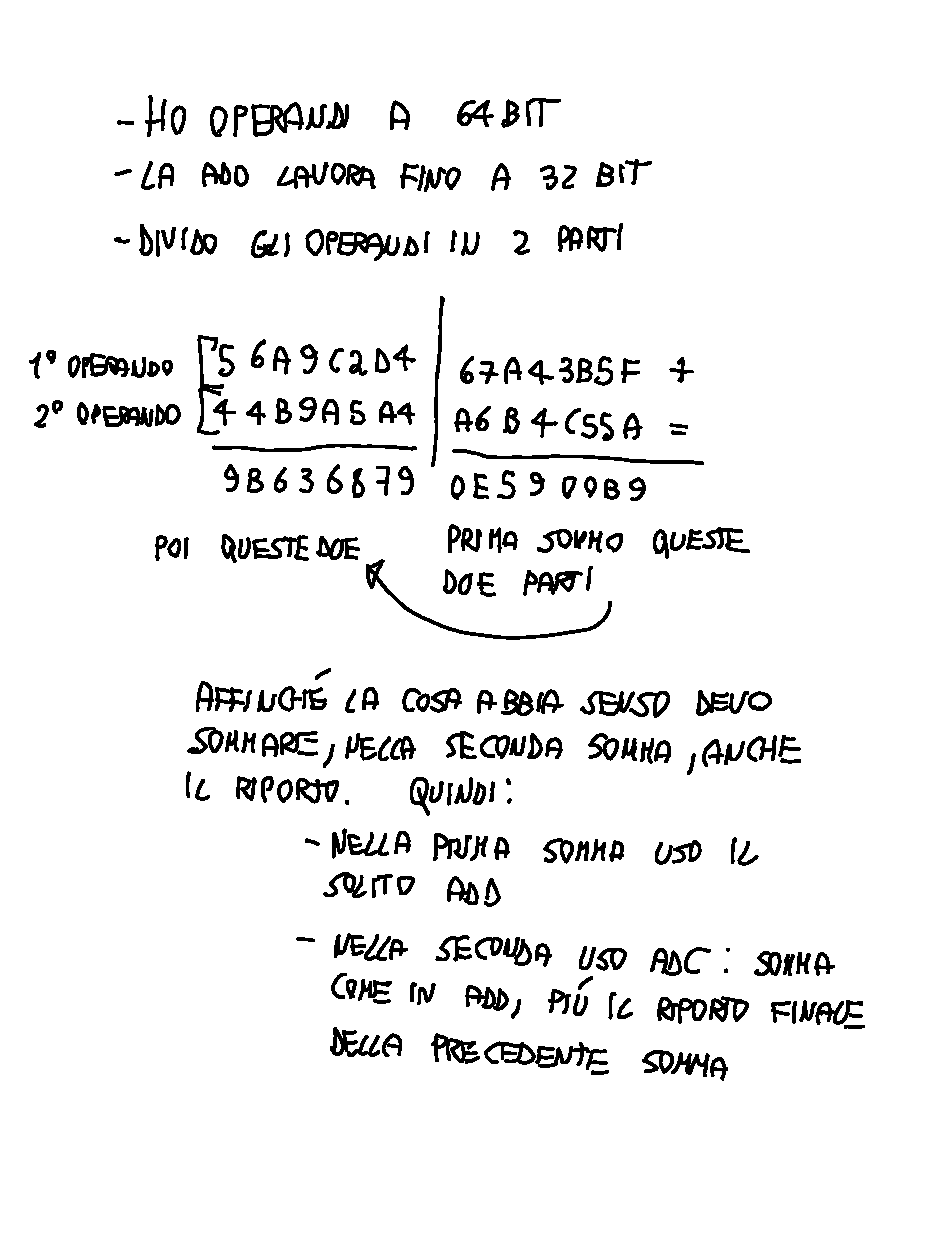
\includepdf[pagecommand={\thispagestyle{plain}},scale=0.70,pages=-]{pdf/pdfsommaa64bit}
\subsection{NEGATE}
\begin{center}
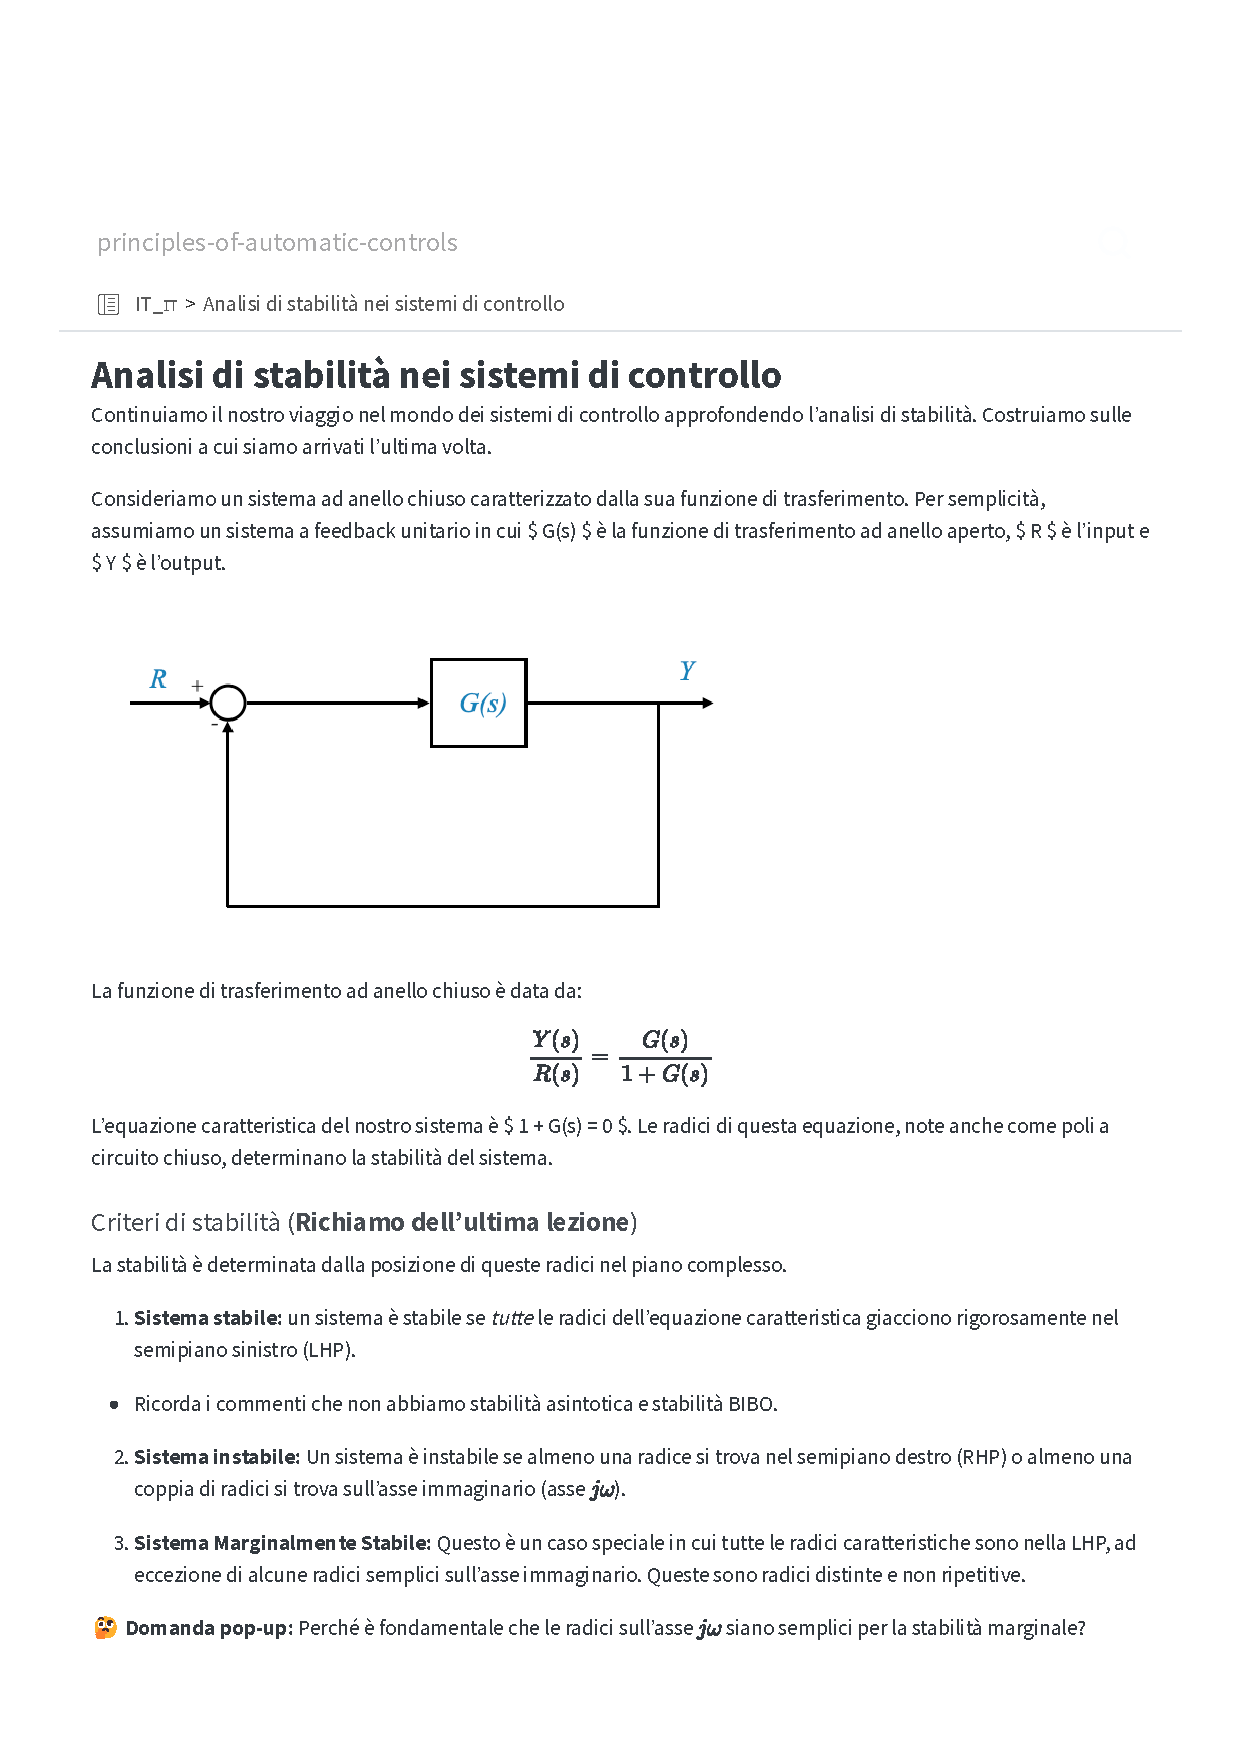
\includegraphics{img/17.PNG}
\end{center}
\paragraph{Algoritmo} Con la NEG si ottiene l'opposto (ovviamente la cosa va fatta con un destinatario concepito come intero) 
\begin{itemize}
\item Complementando bit a bit il destinatario e
\item aggiungendo uno
\end{itemize}
\begin{center}
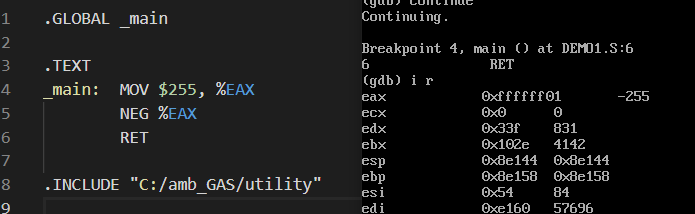
\includegraphics{img/217.PNG}
\end{center}

\paragraph{Attenzione all'overflow} Abbiamo che l'intervallo di rappresentabilità in C2, dato un numero $N$ di bit, è il seguente
\[\left[-2^{N-1};2^{N-1}-1\right]\]
non possiamo calcolare l'opposto dell'estremo negativo ($2^{N-1}$ non appartiene all'intervallo)! In questo caso l'OF sarà uguale ad uno.

\subsection{COMPARE}
\begin{center}
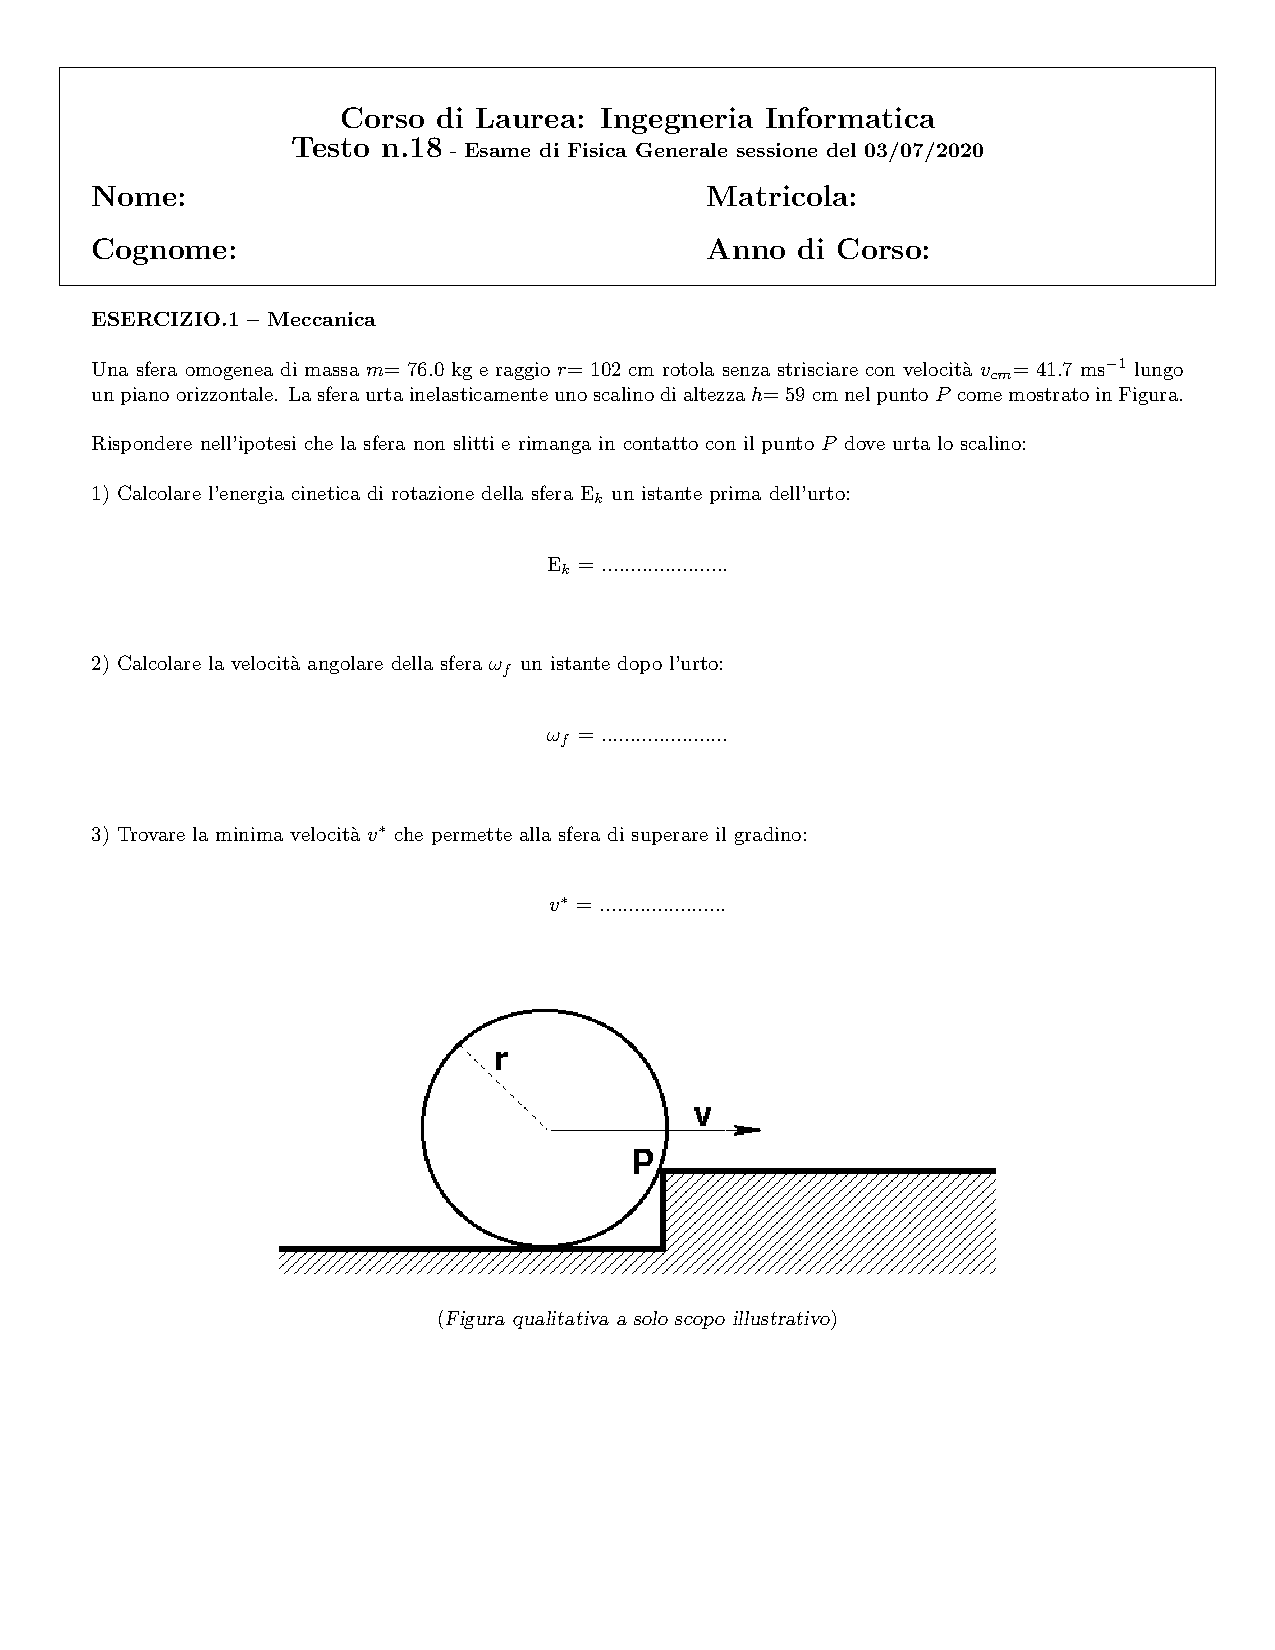
\includegraphics{img/18.PNG}
\end{center}
Presente a pagina 17 della dispensa di Assembler l'algoritmo. Si considera che
\begin{itemize}
\item Con $\text{ZF} = 1$ si ha $\text{destination} = \text{source}$
\item Con $\text{SF} = 1$ si ha risultato della sottrazione negativa, quindi $\text{destination} < \text{source}$
\item Con $\text{SF} = 0$ si ha risultato della sottrazione positiva, quindi $\text{destination} > \text{source}$
\end{itemize}
Noi non controlleremo direttamente i flag ma utilizzeremo delle JUMP CONDIZIONATE. Nella dispensa e nel libro di Corsini sono presenti tutti i JUMP possibili.
\subsection{INTEGER e INTEGER MULTIPLY}
Questa istruzione è concepita diversamente dalle altre operazioni: 
\begin{itemize}
\item Il risultato di una somma sta su $N$ o $N+1$ cifre
\item Il prodotto di due numeri a $N$ cifre sta su $2N$ cifre. Questo dettaglio pone un problema non secondario: contrariamente alla somma non posso comparare fattori e risultato. Segue che un operando non potrà essere utilizzato sia come fattore che come risultato.
\end{itemize}
Potrei pensare a un'istruzione a tre operandi, ma cose del genere in assembler non esistono. Si risolve specificando un solo operando (l'operando sorgente): l'altro operando e la sede del risultato sono impliciti. Si osserva che i risultati delle moltiplicazioni, in 16 e 32bit, vengono divisi tra due registri. In 32bit la cosa è necessaria, ma in 16bit a cosa serve? Non potrei fare...?
\begin{verbatim}
EAX=AX* source
\end{verbatim}
Anche in questo caso le motivazioni sono storiche: i registri precedentemente erano a 16bit, e il ragionamento che si faceva era lo stesso fatto con gli operandi a 32bit. Con l'estensione dei registri si è mantenuta la cosa per compatibilità.
Un trucco per porre il risultato in un registro a 32bit è il seguente
\begin{verbatim}
PUSH %DX
PUSH %AX
POP %EAX
\end{verbatim}
Pongo nella pila prima la parte alta (cifre più significative), poi la parte bassa (cifre meno significative), poi le estraggo dalla pila insieme (nei comandi push abbiamo indicato due registri a 16bit, col comando pop indichiamo un registro a 32bit).
\begin{center}
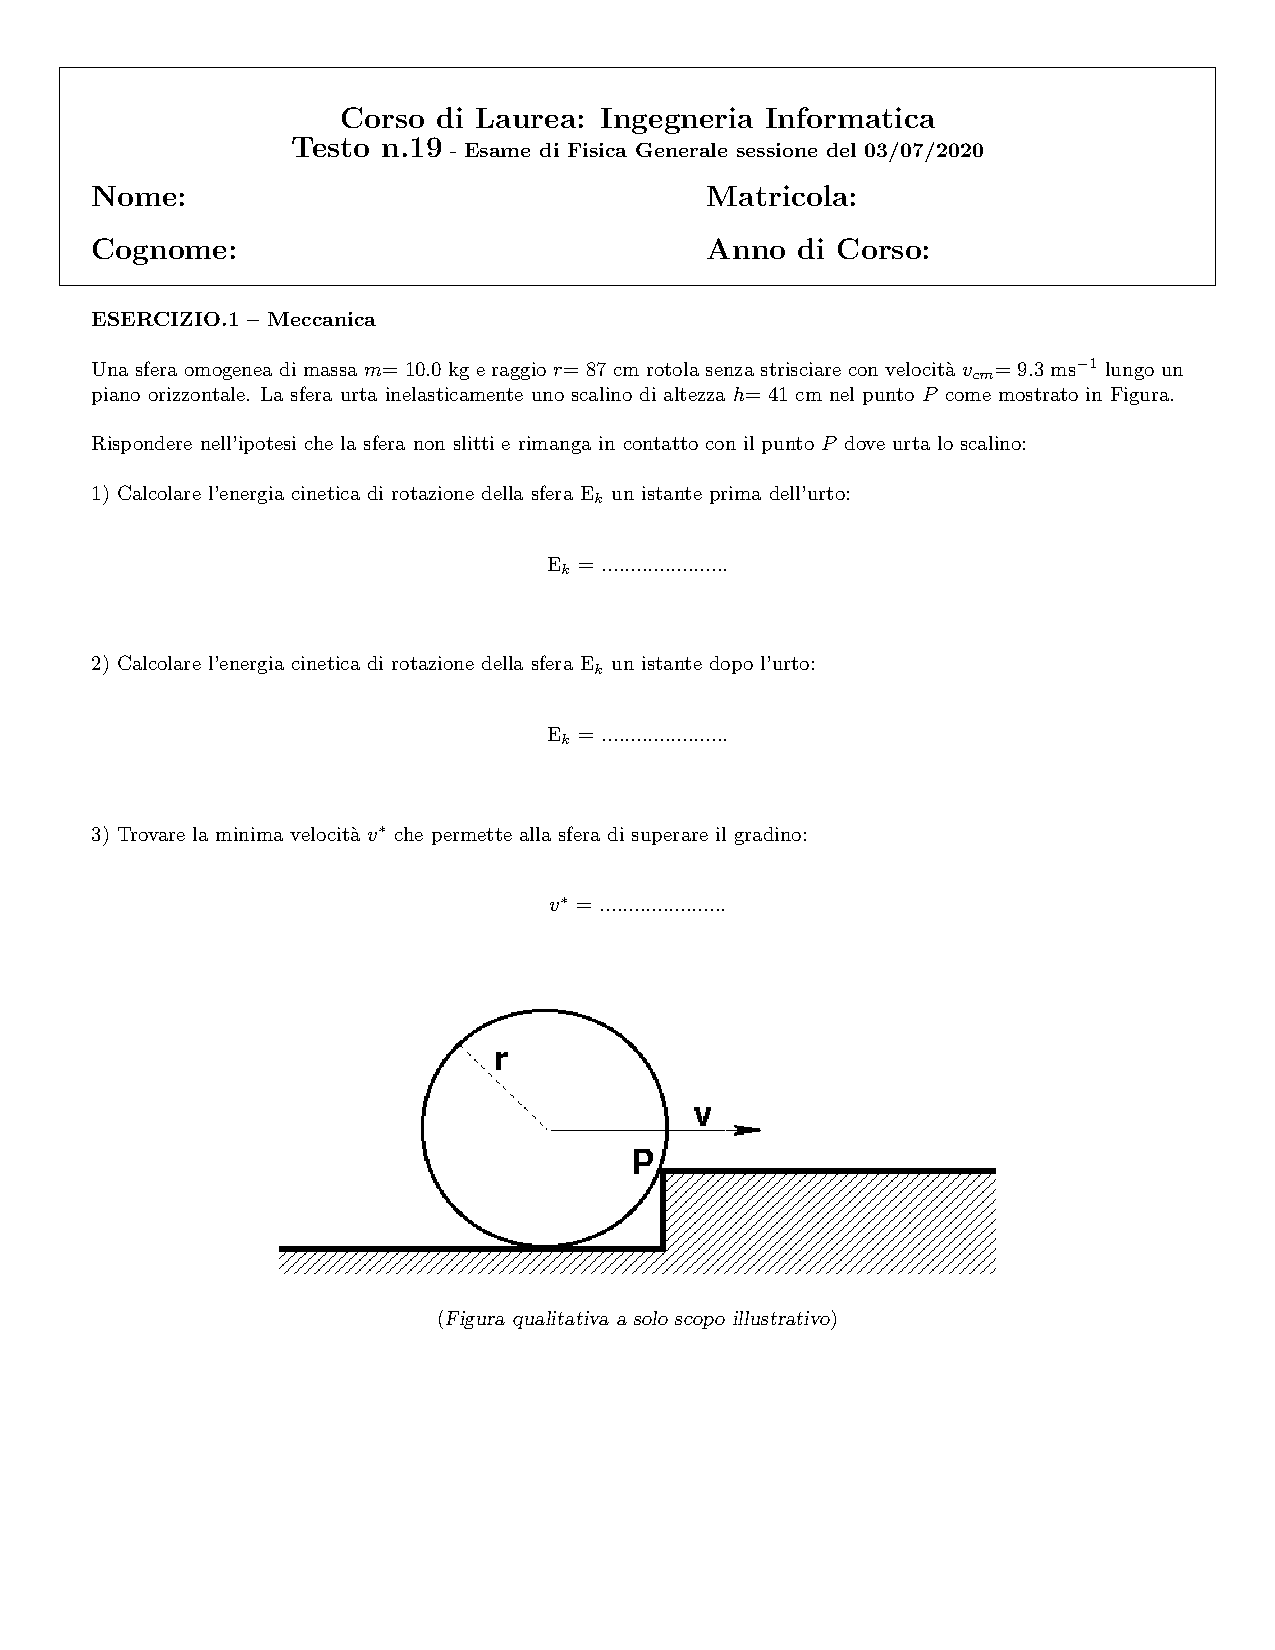
\includegraphics{img/19.PNG}
\end{center}
\begin{center}
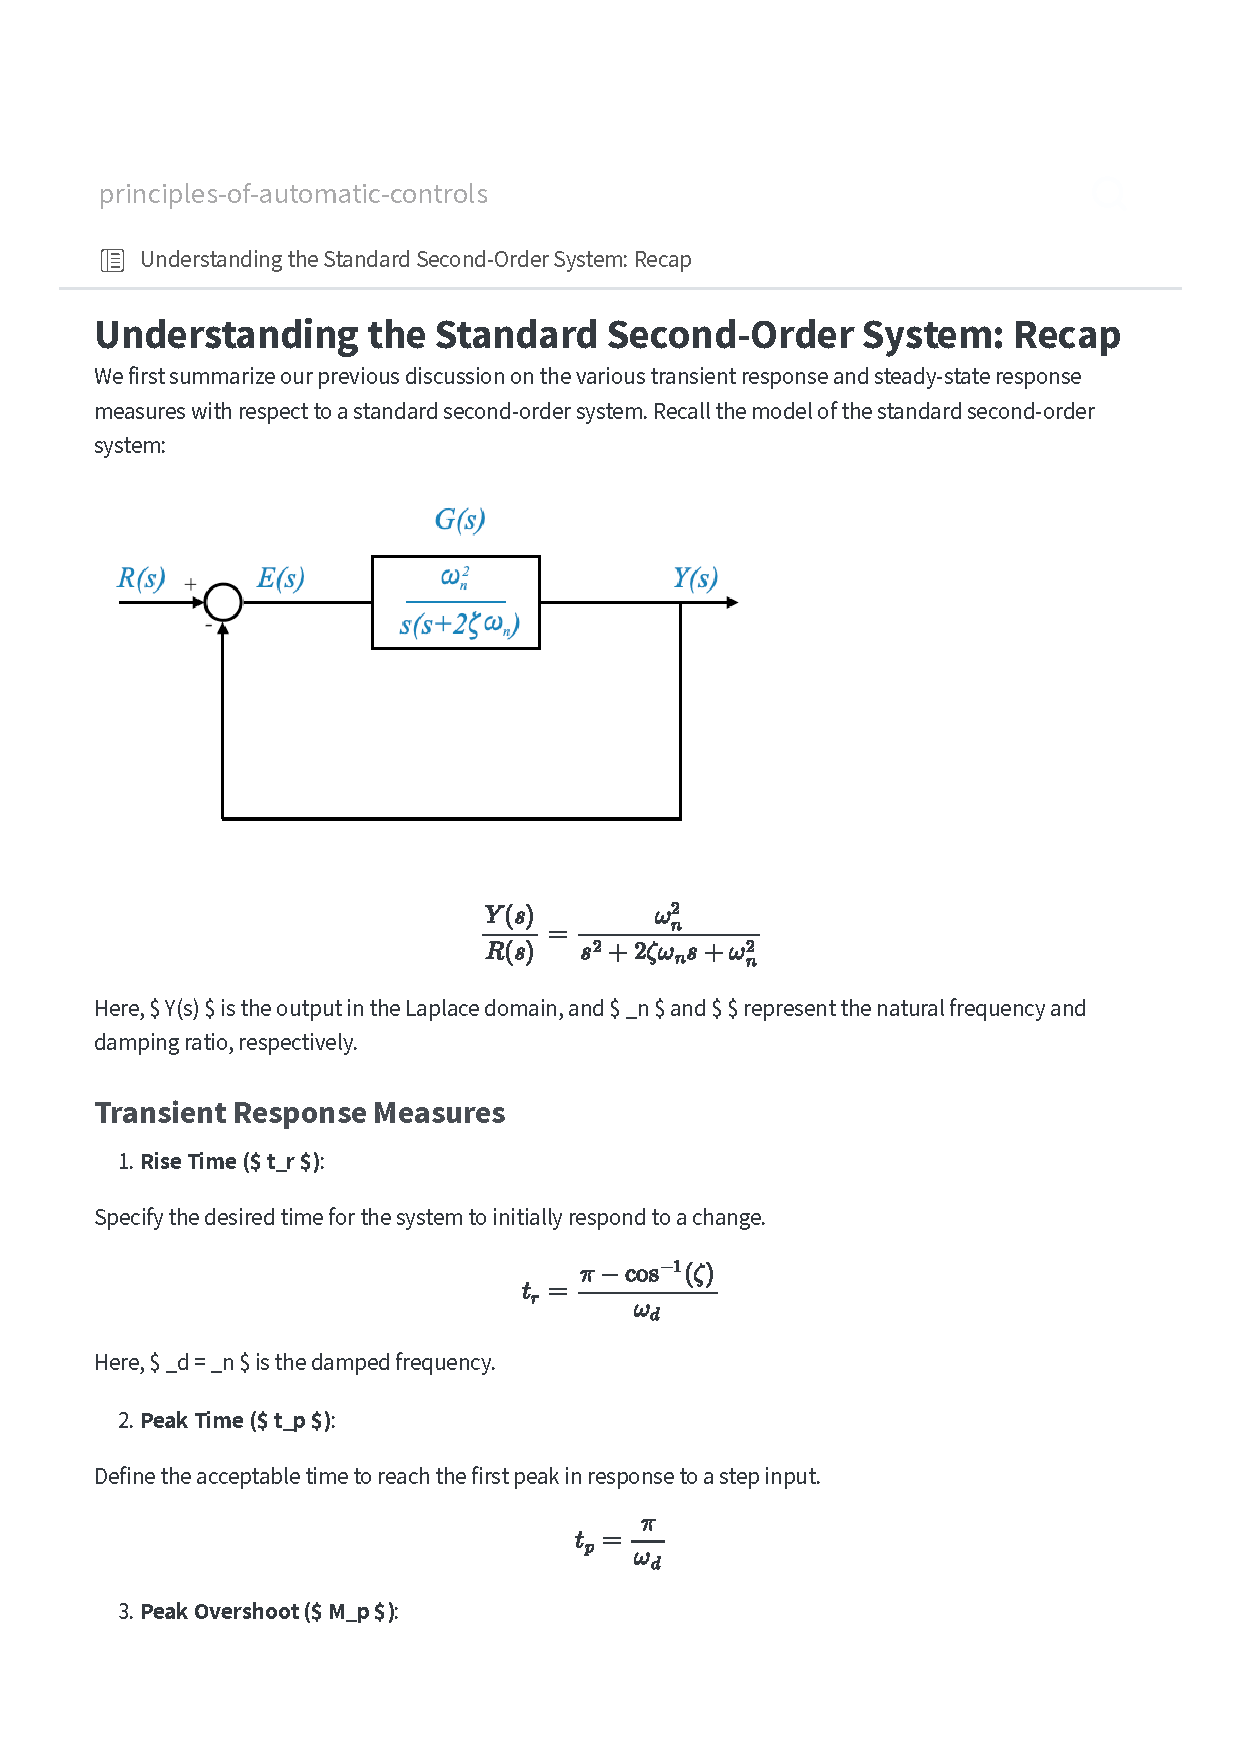
\includegraphics{img/20.PNG}
\end{center}
\paragraph{Quindi}
\begin{itemize}
\item Uno dei due operandi è un registro, l'altro è indicato nell'istruzione (source)
\item L'operando source determina il numero di bit che andremo ad utilizzare per il risultato, quindi i registri dove saranno salvati i risultati.
\item Se source è a 16 o 32 bit i risultati saranno divisi tra due registri: con 32bit è necessario, in 16bit si ha questa cosa per ragioni storiche.
\end{itemize}
\paragraph{Non attendibile?} Molto difficile da capire cosa succeda coi flag. Inutile guardare, non ci dovrebbero servire (cit.Stea)
\subsection{DIVIDE e INTEGER DIVIDE}
La divisione presenta qualche problemino ulteriore rispetto alla moltiplicazione:
\begin{itemize}
\item I risultati sono due: quoziente e resto
\item l'operazione non è fattibile se il divisore vale zero.
\end{itemize}
Dato un dividendo $X$ e un divisore $Y$ individuiamo che $0\leq R \leq Y-1$ (può essere grande quanto il divisore) e $0 \leq Q \leq X$ (può essere grande quanto il dividendo).
\paragraph{Istruzione} Il risultato è diviso tra due registri in tutte le versioni possibili. Ricordiamo che dobbiamo salvare quoziente e divisore.
\paragraph{Osservazione} Risulta ovvio che la dimensione del divisore (source) risulta inferiore al dividendo. 
\begin{itemize}
\item Se il divisore è di 8bit il dividendo sarà di 16bit
\item Se il divisore è di 16bit il dividendo sarà di 32bit
\item Se il divisore è di 32bit il dividendo sarà di 64bit
\end{itemize}
negli ultimi due casi il dividendo sarà preso dai due registri divisi.
\paragraph{Wait} Ma non si era detto che il quoziente può stare al massimo nel numero di bit del dividendo? Cosa succede se il quoziente non è rappresentabile sul registro designato? Se il quoziente della divisione non sta sul numero di bit previso dal formato viene sollevata un'eccezione (la stessa eccezione che partirebbe con una divisione per 0 - il programma si inchioda). Per evitare problemi del genere dobbiamo scegliere un'adeguata versione della divisione
\paragraph{Esempio di divisione} Supponiamo di voler fare 15.000 per 3 (abbiamo un dividendo di 16bit e un divisore di 8bit). Se noi dividiamo otteniamo come risultato 5000. Questo è problematico se adottiamo la divisione con source ad 8bit, segue che le seguenti istruzioni non vanno bene!
\begin{verbatim}
MOX $3, %CL
MOV $15000, %AX
DIV %CL
\end{verbatim}
La cosa può essere risolta così:
\begin{verbatim}
MOX $3, %CX
MOV $15000, %AX
MOV $0, %DX <---------------
DIV %CX
\end{verbatim}
Abbiamo modificato il contenuto dei registri $AX$ e $DX$: questo è sufficiente per scegliere la divisione con source a 16bit. La terza istruzione è vitale, e molto spesso viene dimenticata (cit.)
\begin{center}
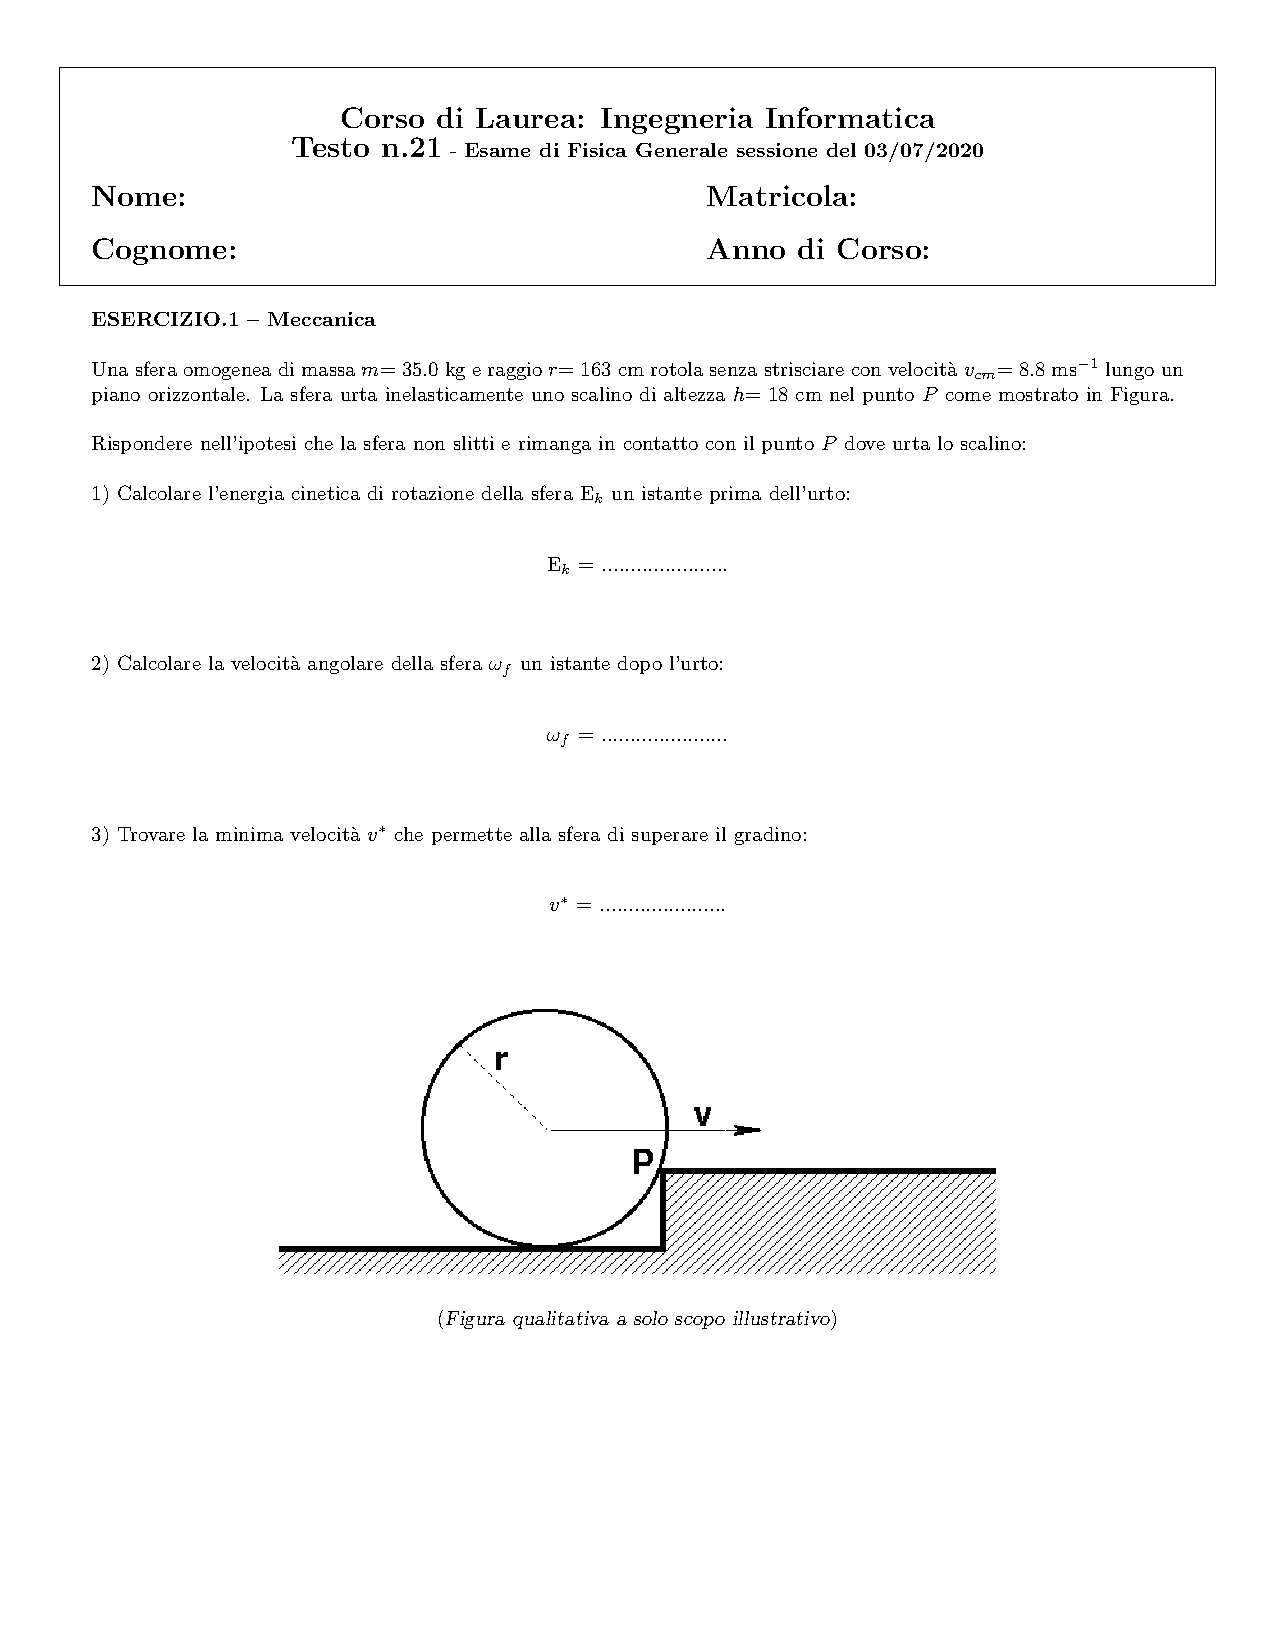
\includegraphics{img/21.PNG}
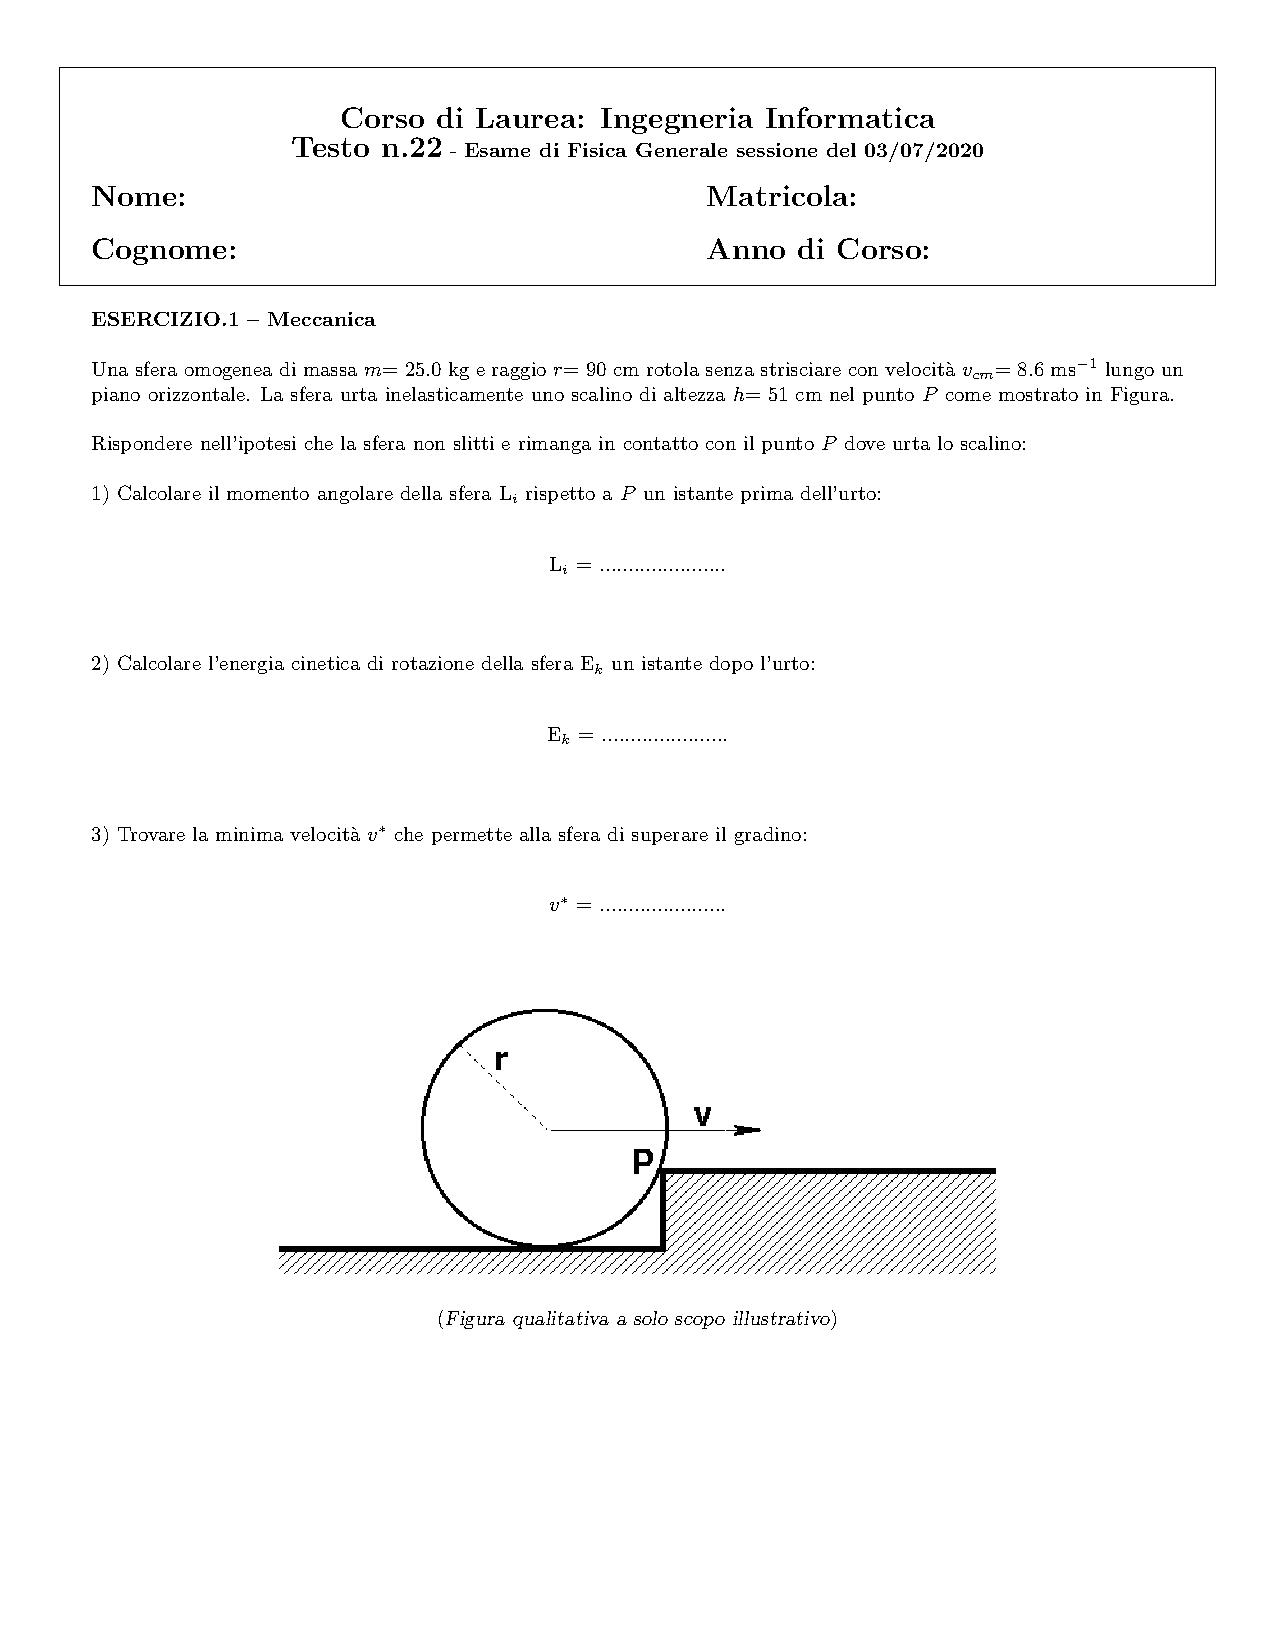
\includegraphics{img/22.PNG}
\end{center}
\paragraph{Divisione intera} 
\begin{itemize}
\item Nella divisione intera il resto ha sempre il segno del dividendo e in modulo è minore rispetto a quello del divisore. 
\begin{center}
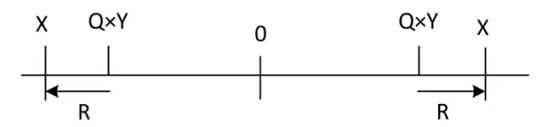
\includegraphics{img/199.PNG}
\end{center}
\begin{verbatim}
-7 idiv 3 : quoziente -2, resto -1
 7 idiv -3: quoziente -2, resto +1
\end{verbatim}
\item Ciò significa che il quoziente viene approssimato per troncamento, cioè viene sempre approssimato all'intero più vicino allo zero. In entrambi gli esempi ottengo che $Q \times Y$, cioè il prodotto tra quoziente e divisore, è più vicino allo zero rispetto al dividendo.
\item La cosa è inconsistente con le nozioni di algebra che conosciamo: per capire la differenza pensiamo alla definizione di resto.
\[|-4|_3=|3 \cdot (-2) + 2|_3=|2|_3=2\,\,\,\,\,\,\,\,\,\,\,\,\,\,|4|_3=1\]
\end{itemize}
\subsection{Conclusioni}
\begin{itemize}
\item Scegliere con cura la versione della divisione (basandoci sulle ipotesi in mano nostra)
\item I registri devono essere azzerati prima del calcolo, altrimenti i risultati potrebbero essere inconsistenti (chi ce lo dice che il registro con le cifre più significative presenti bit nulli?)
\item Ricordarsi che il contenuto di DX o EDX viene modificato dalle operazioni
\end{itemize}
Per la moltiplicazione:
\begin{itemize}
\item Se l'unico operando esplicito (un fattore) è a 8bit allora il risultato della moltiplicazione (l'altro fattore è un registro a 8bit) sarà posto in un registro a 16bit.
\item Se l'unico operando esplicito (un fattore) è a 16bit allora il risultato della moltiplicazione (l'altro fattore è un registro a 16bit) sarà diviso in due registri a 16 bit (abbiamo quindi un risultato a 32bit).
\item Se l'unico operando esplicito (un fattore) è a 32bit allora il risultato della moltiplicazione (l'altro fattore è un registro a 32bit) sarà diviso in due registri a 32 bit (abbiamo quindi un risultato a 64bit).
\end{itemize}
Per la divisione:
\begin{itemize}
\item Se l'unico operando esplicito (divisore) è a 8bit allora quoziente e resto saranno memorizzati su registri a 8bit (il dividendo è a 16bit).
\item Se l'unico operando esplicito (divisore) è a 16bit allora quoziente e resto saranno memorizzati su registri a 16bit (il dividendo è a 32 bit, diviso su due registri).
\item Se l'unico operando esplicito (divisore) è a 32bit allora quoziente e resto saranno memorizzati su registri a 32bit (il dividendo è a 64bit, diviso su due registri).
\end{itemize}

\chapter{Venerdì 02/10/2020}
\section{Continuiamo con le istruzioni aritmetiche}
\subsection{Estensione di campo}
Con estensione di campo intendiamo un'operazione con cui si rappresenta un numero usando più cifre.
\subsection{Naturali}
Nei numeri naturali l'operazione è banale, mi basta aggiungere gli zeri a sinistra. Segue una cosa del seguente tipo
\[100110 \longrightarrow \boxed{0}100110\]
\subsection{Interi}
Nei numeri interi non possiamo fare la stessa cosa: il MSB indica il segno, quindi non posso aggiungere zeri (andrei ad alterare il segno del numero). Il metodo adottato consiste nel ripetere il bit più significativo
\[100110 \longrightarrow \boxed{1}100110\]
Il motivo di questo metodo è chiaro quando passiamo da rappresentazione in base 2 di un intero negativo alla base 10.
\subsection{CONVERT WORD TO DOUBLEWORD in EAX}
\begin{center}
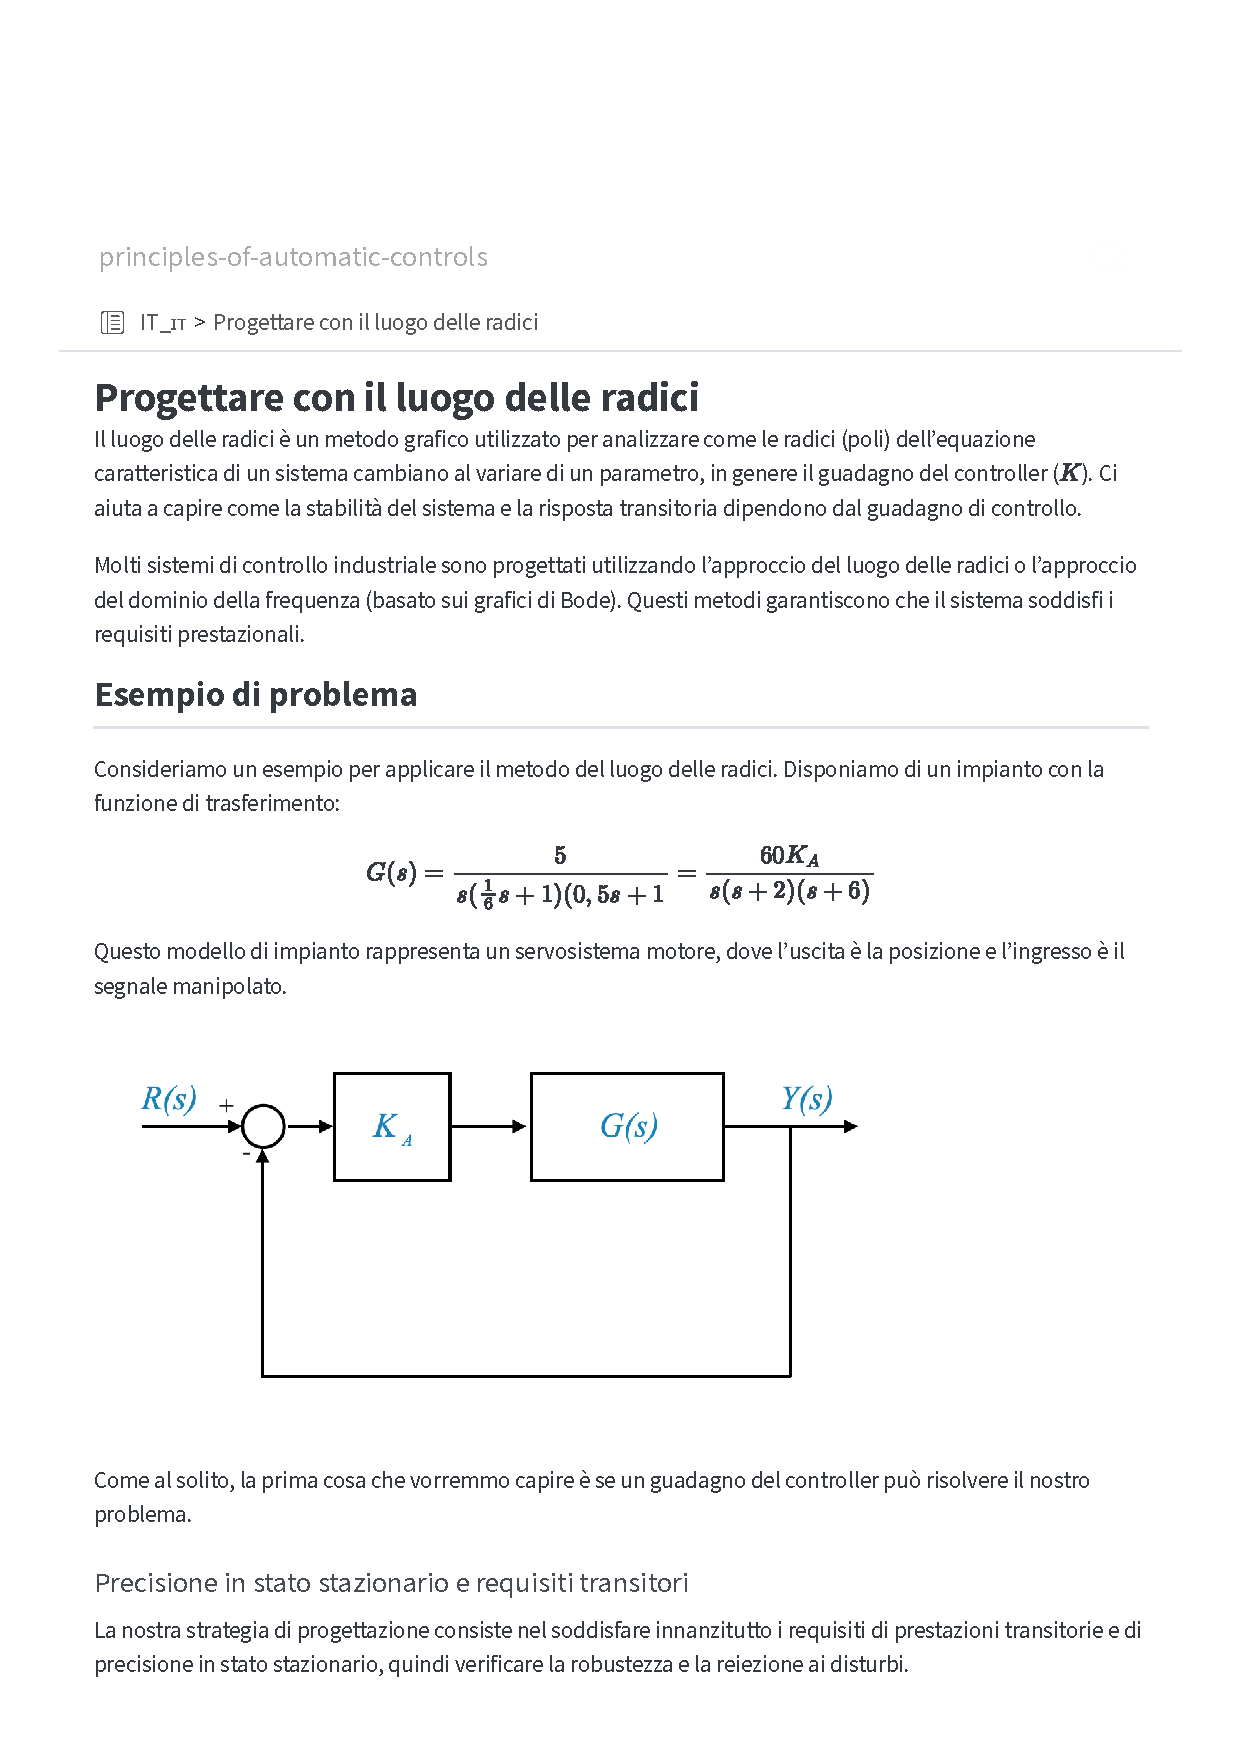
\includegraphics{img/23.PNG}
\end{center}

\section{Istruzioni di traslazione}
Le istruzioni di traslazione permettono la variazione dell'ordine di bit in un operando destinatario. Solitamente si hanno due formati
\begin{verbatim}
OPCODE src, dest
OPCODE dest
\end{verbatim}
col primo formato indichiamo, attraverso src (immediato o registro CL, di cui si considerano solo i 5bit più bassi), quante volte vogliamo ripetere l'operazione; col secondo ci limitiamo ad eseguire l'operazione una sola volta (è come se ponessi $\text{src}=1$). Ovviamente src deve valere al più 31: porre un $\text{src} > 31$ ha poco senso.

\subsection{SHIFT LOGICAL LEFT}
\begin{center}
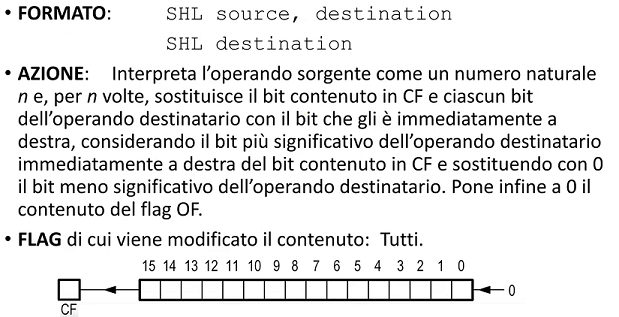
\includegraphics{img/24.PNG}
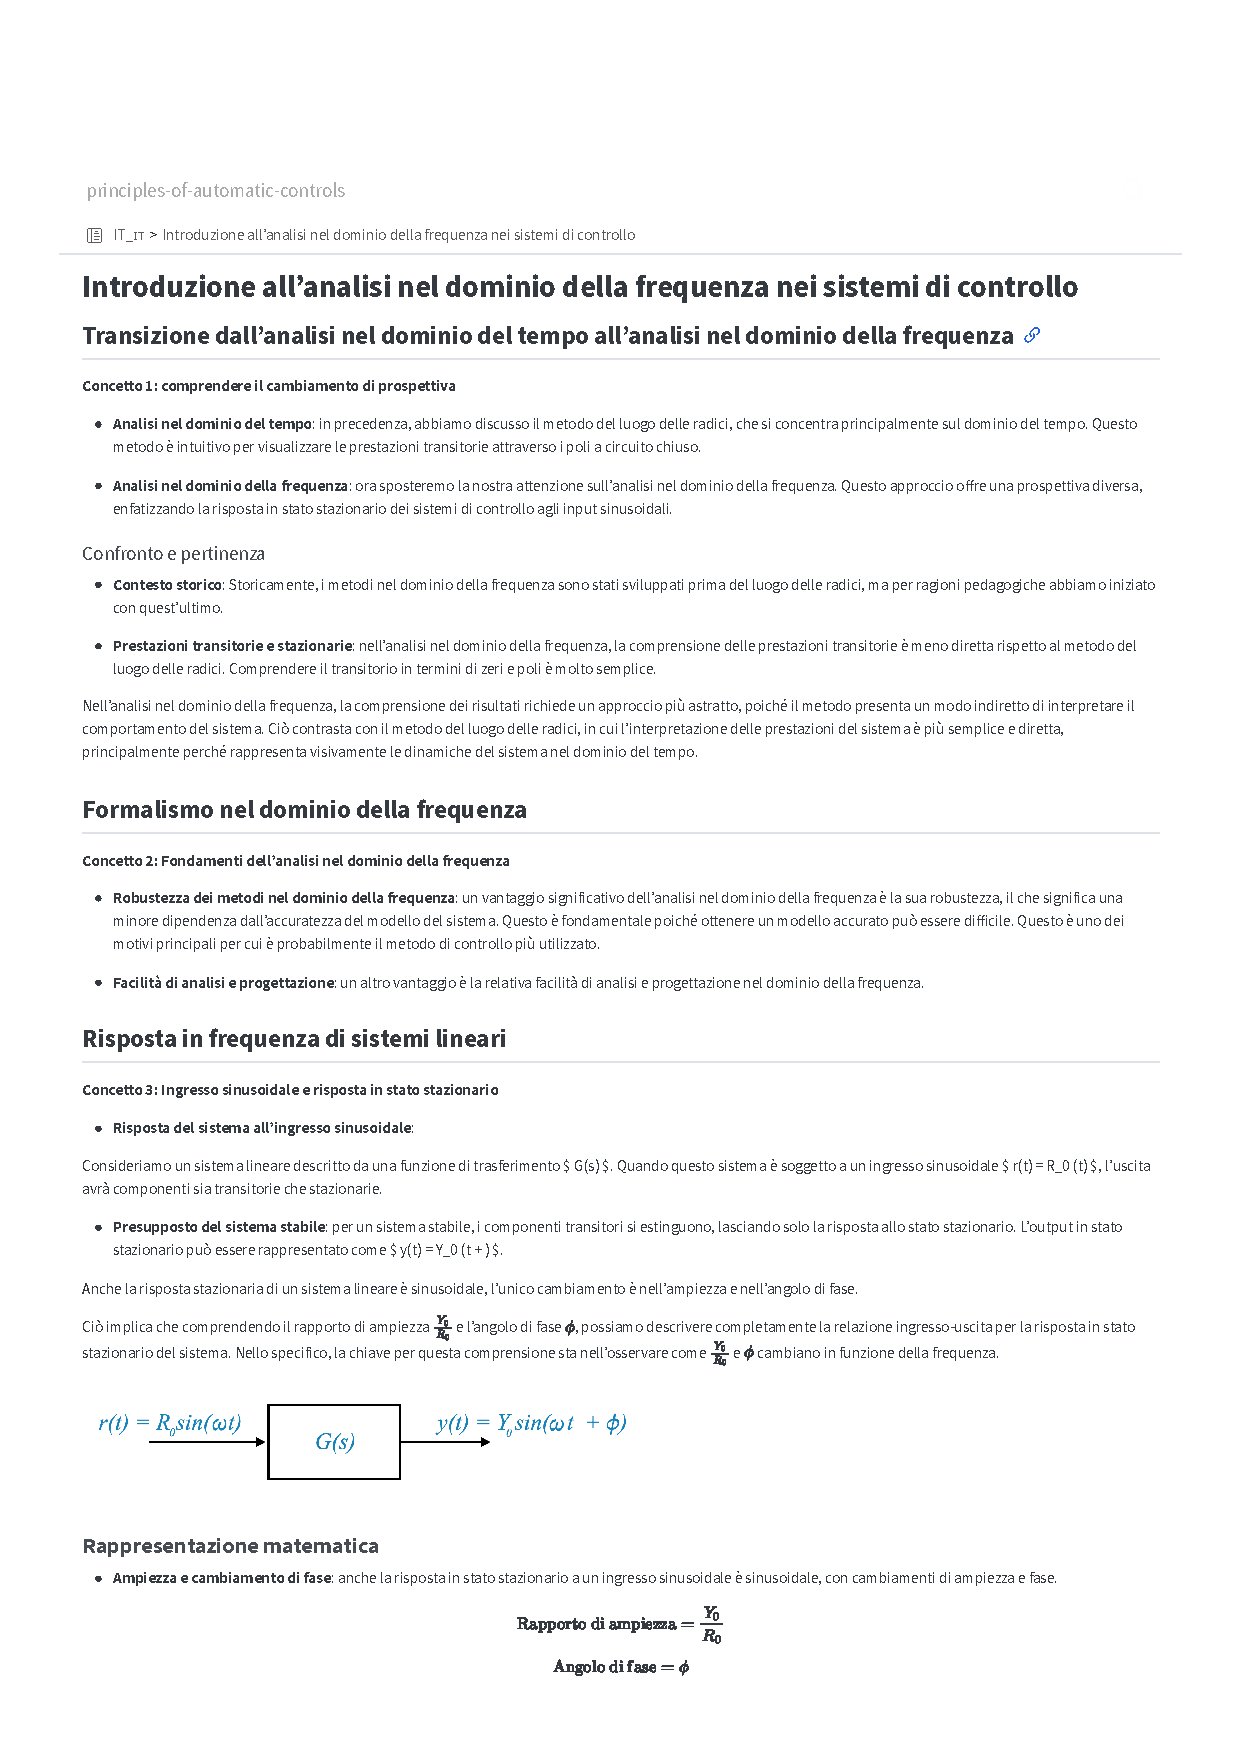
\includegraphics{img/25.PNG}
\end{center}
\paragraph{Attenzione} In alcuni casi lo shift può essere utile sul piano dell'efficienza (occupo meno spazio con l'operazione ed eseguo un'operazione più veloce). In altri casi può essere una condanna a morte: quando si utilizza questa istruzione ci si sbarazza ogni volta di un bit, quindi si perde informazione. Segue che una moltiplicazione per $2^3=8$  sia possibile con lo shift left solo se il risultato non esce dal numero di bit a disposizione.
\subsection{SHIFT ARITHMETIC LEFT}
\begin{center}
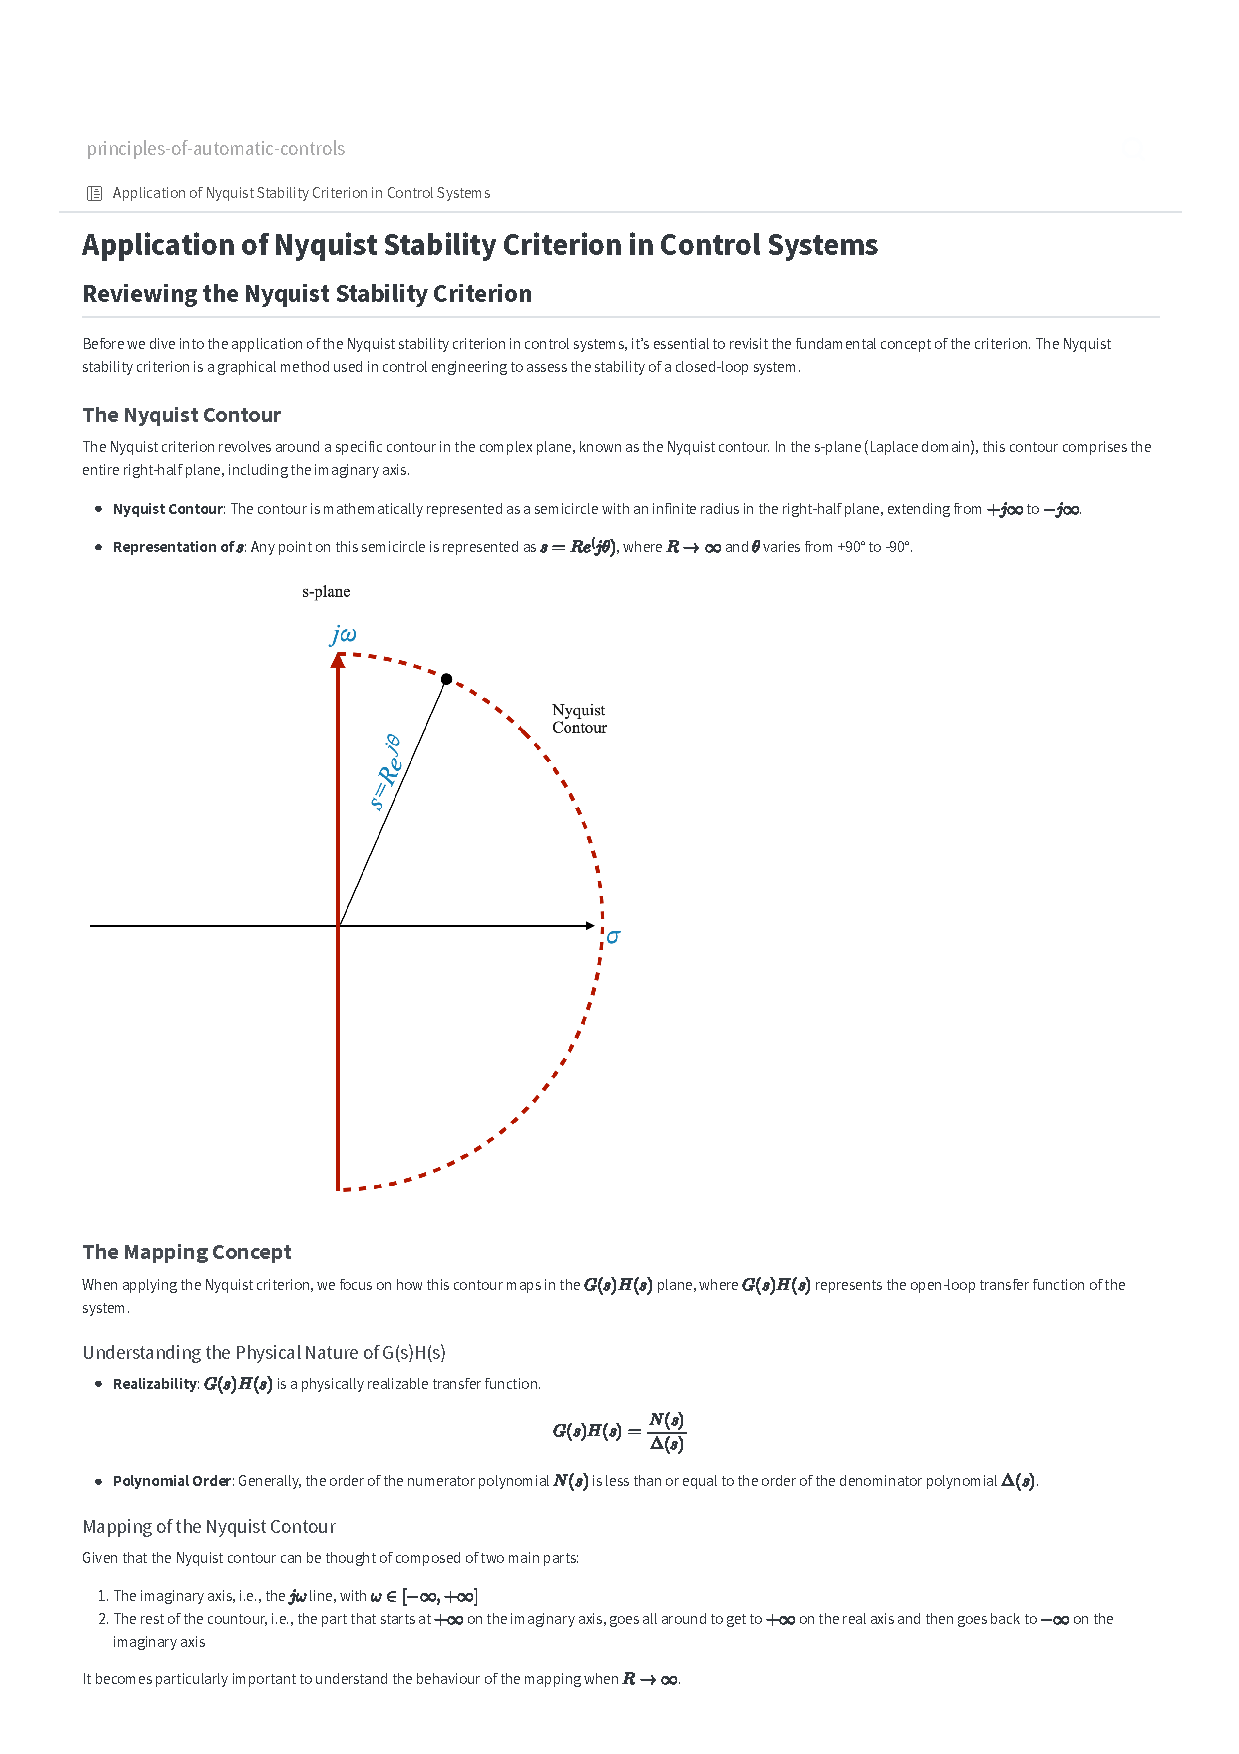
\includegraphics{img/26.PNG}
\end{center}

\subsection{SHIFT LOGICAL RIGHT}
\begin{center}
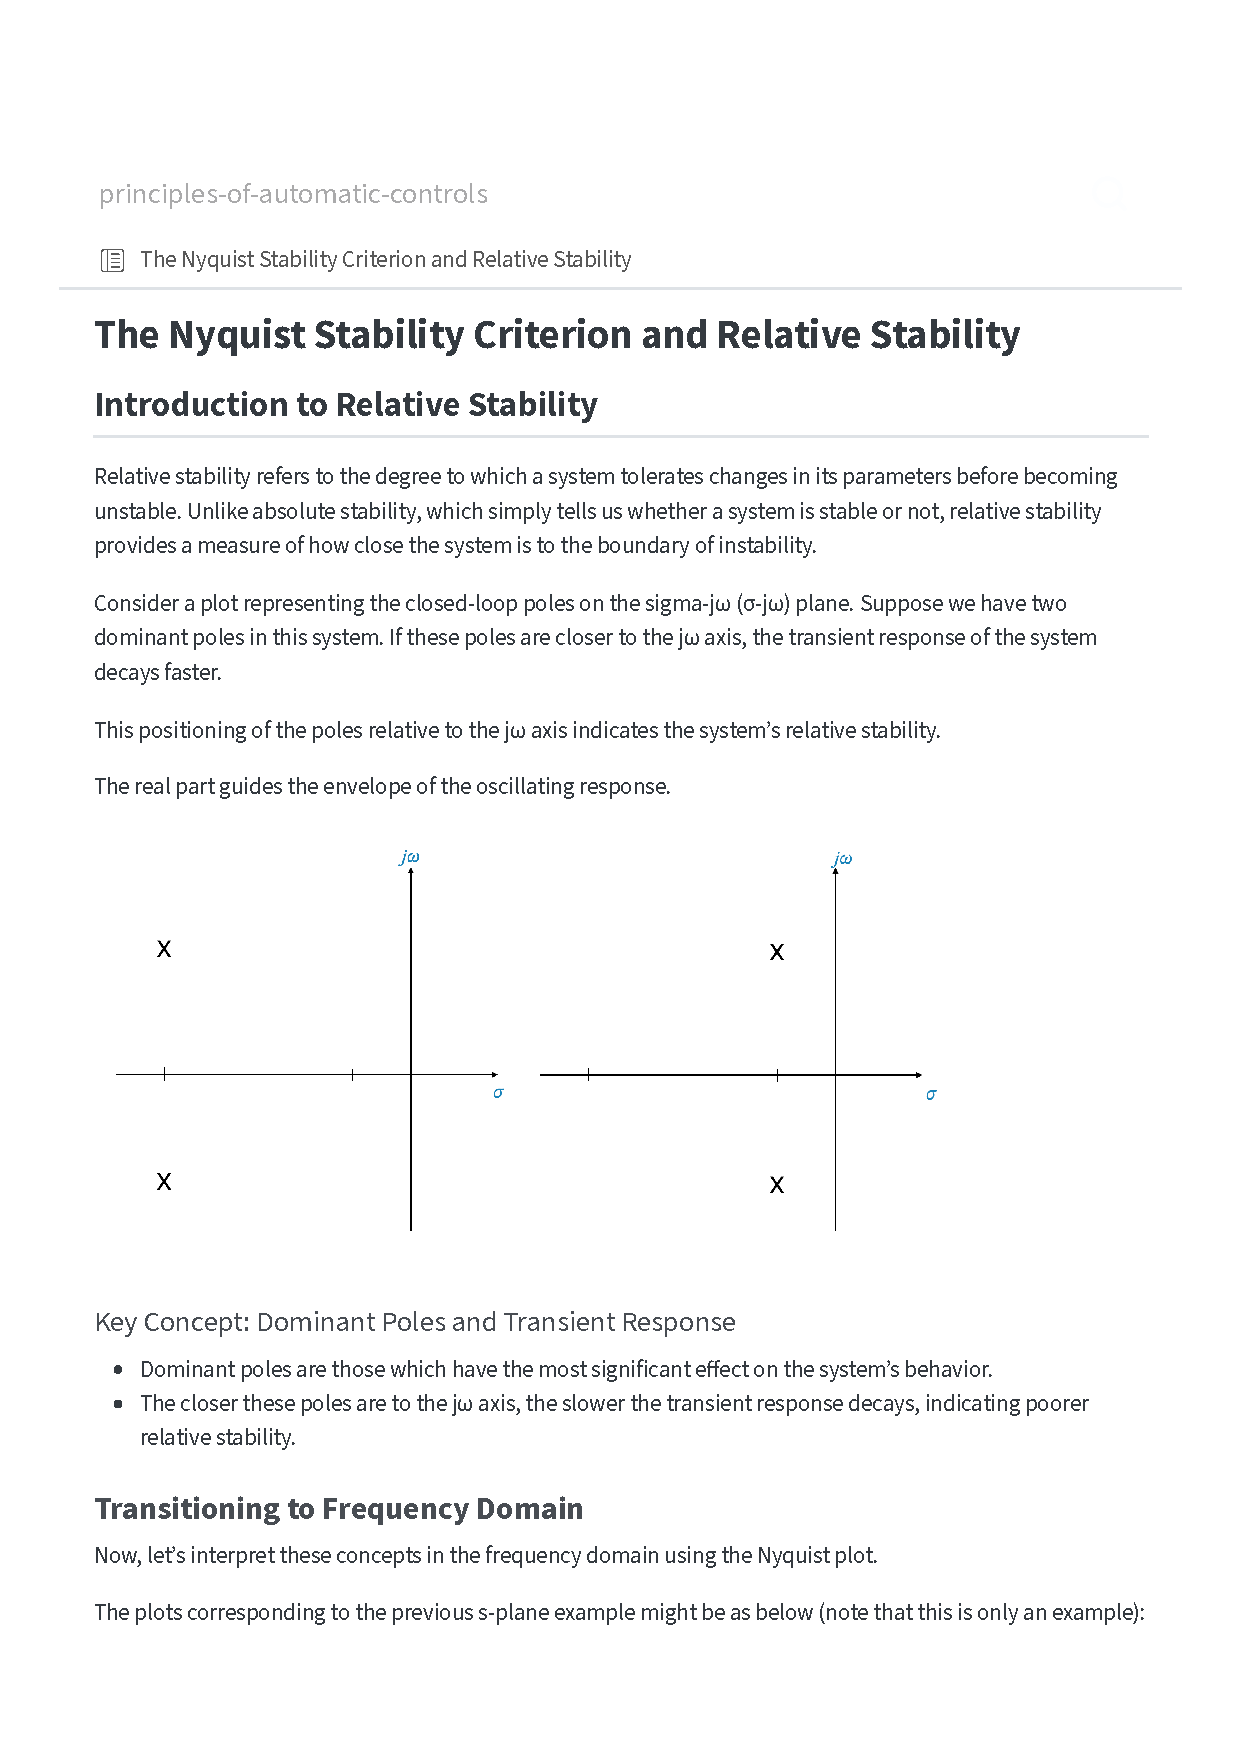
\includegraphics{img/27.PNG}
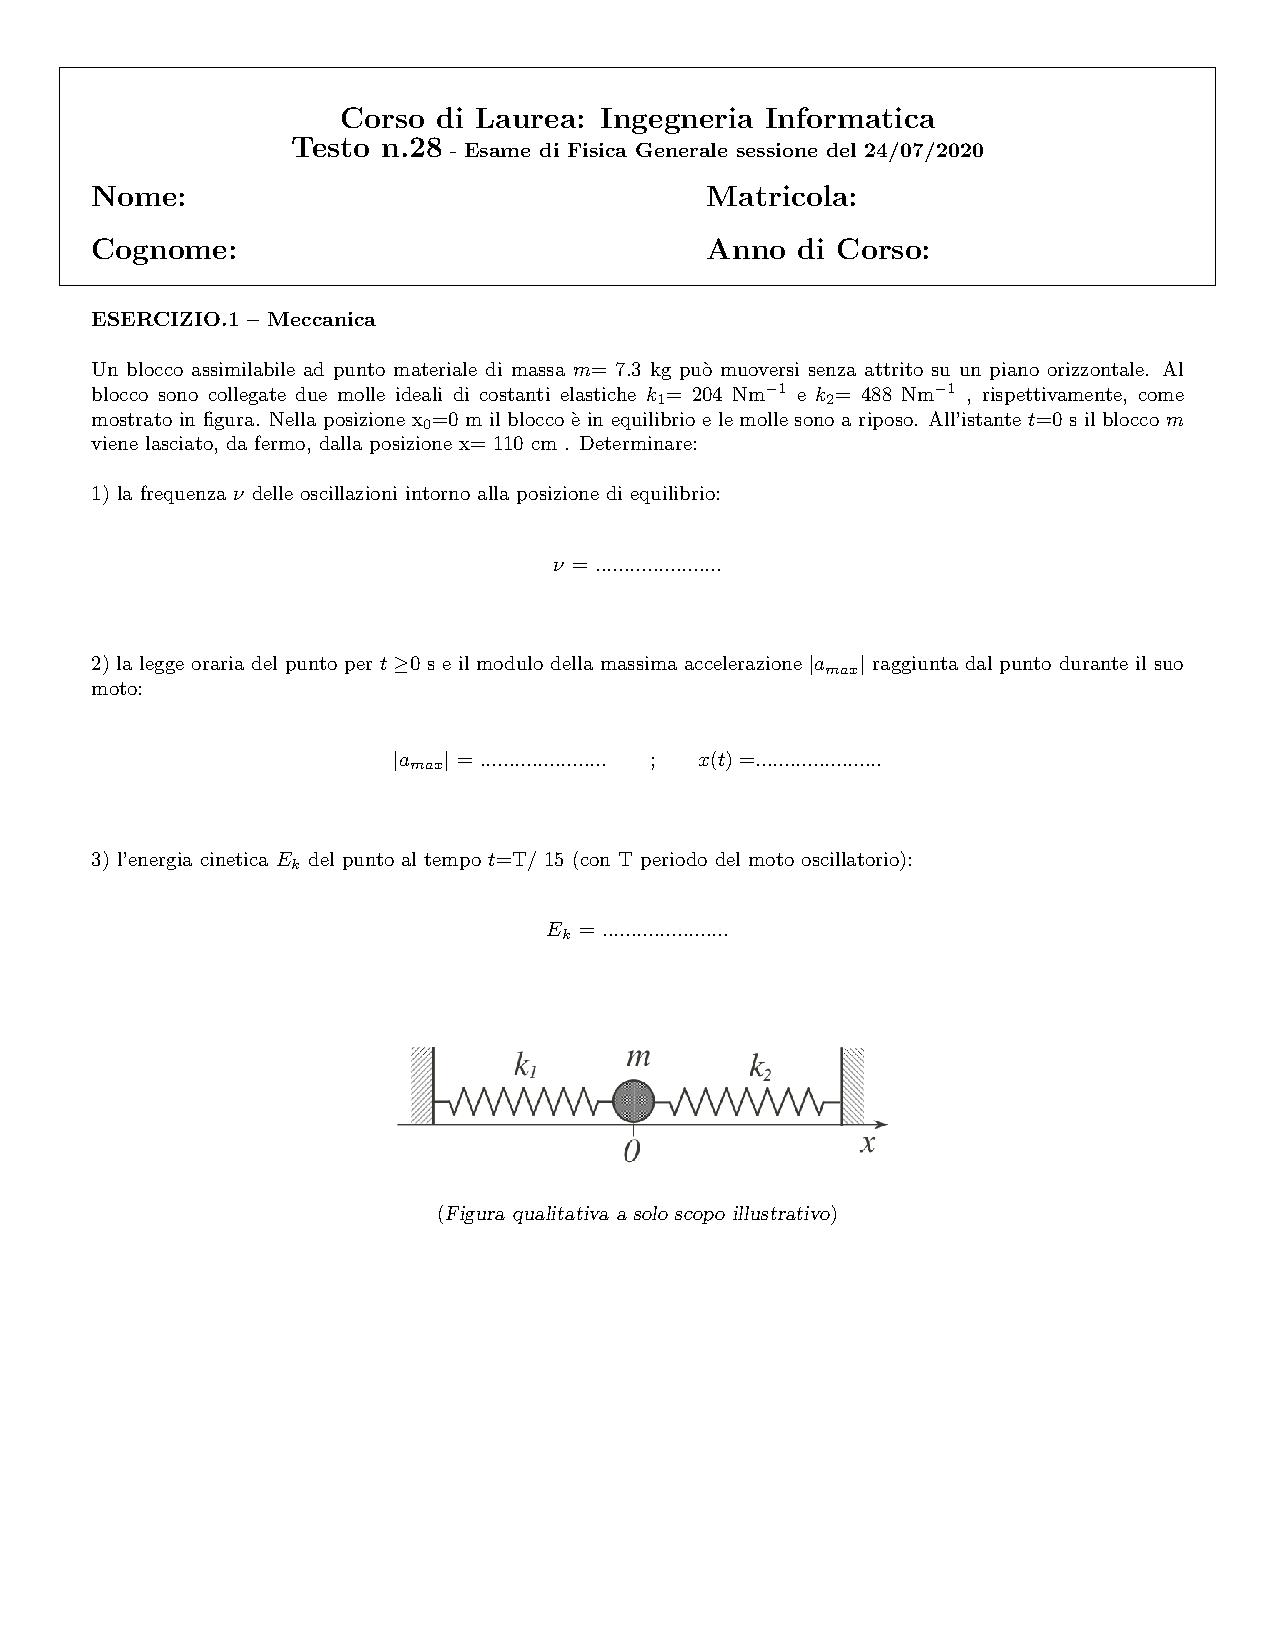
\includegraphics{img/28.PNG}
\end{center}

\subsection{SHIFT ARITHMETIC RIGHT}
Non è possibile applicare lo stesso algoritmo agli interi: abbiamo già detto che negli interi il MSB rappresenta il segno del numero, segue che non posso fare entrare zeri a sinistra come in SHIFT LOGICAL RIGHT
\begin{center}
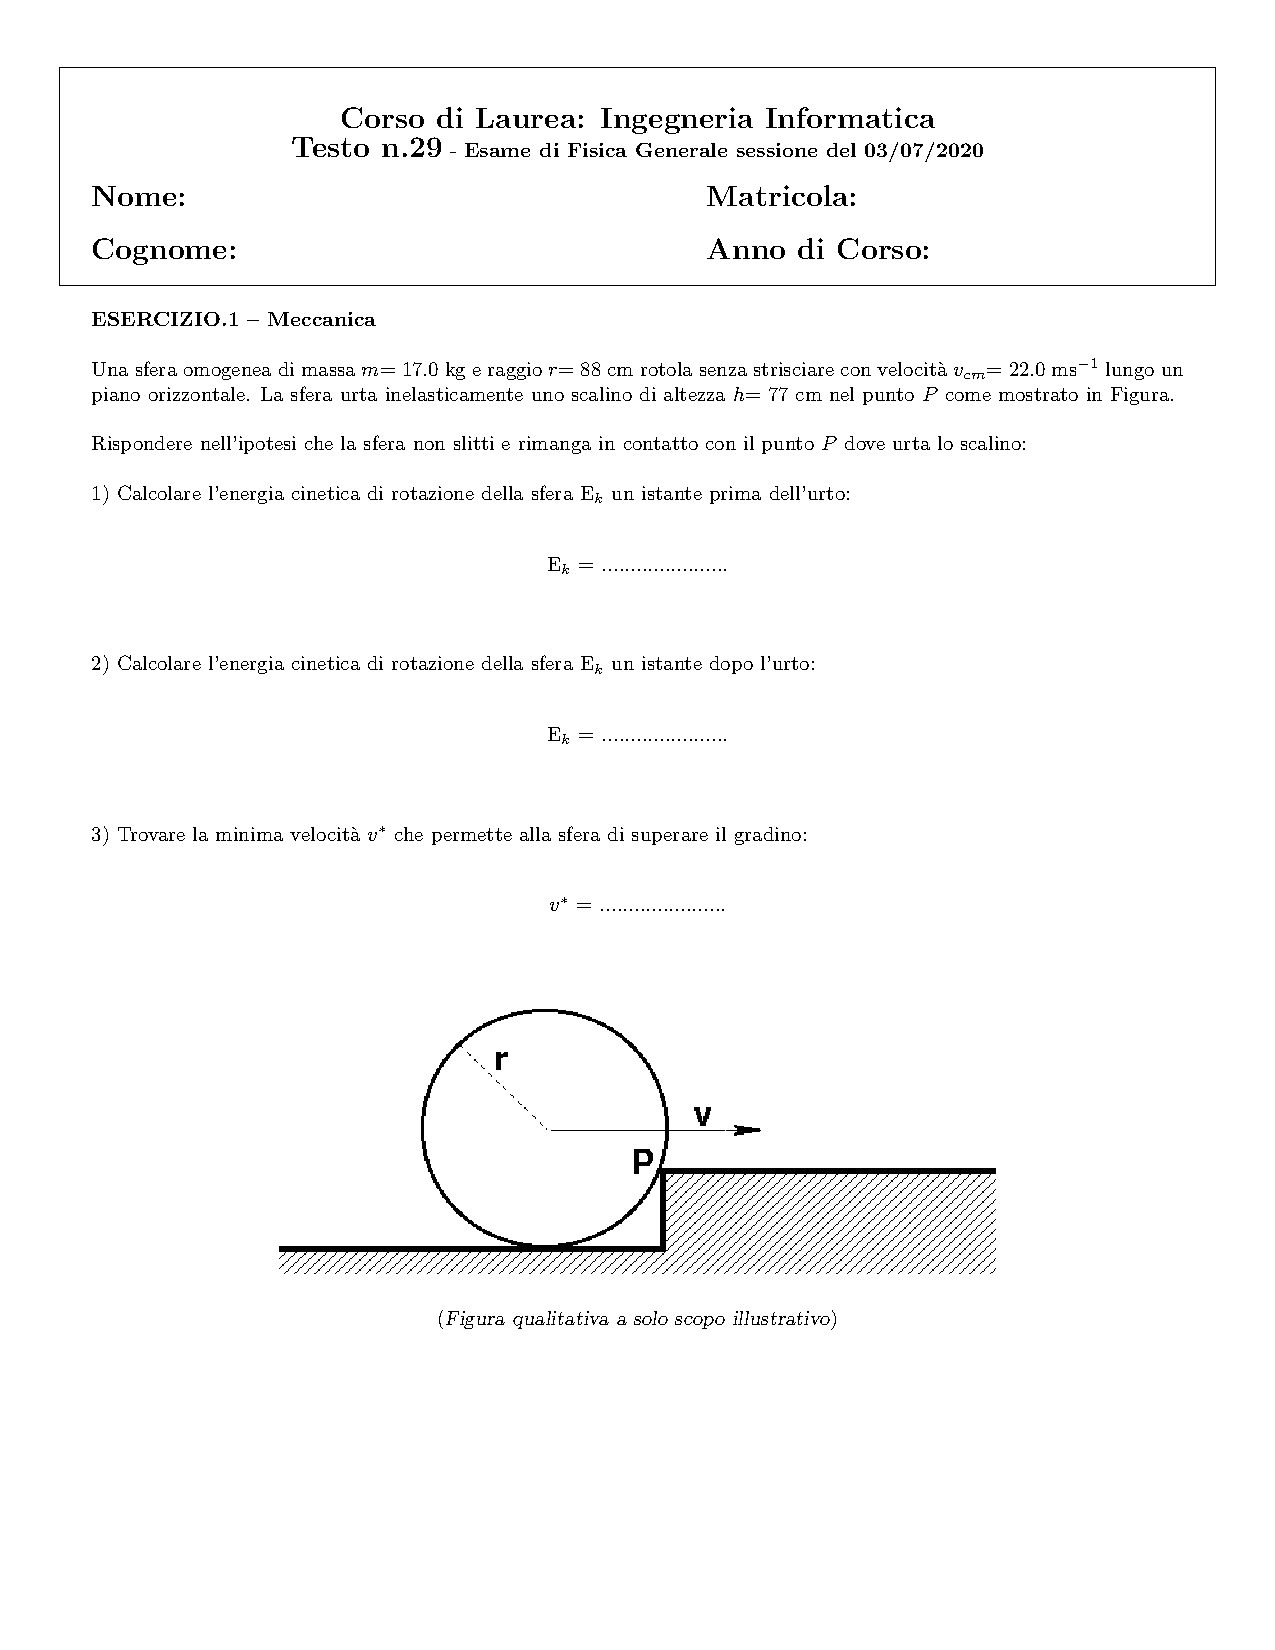
\includegraphics{img/29.PNG}
\end{center}
\paragraph{Attenzione al quoziente} SAR e IDIV restituiscono lo stesso quoziente quando il dividendo è positivo oppure quando la divisione da resto nullo. Casi diversi sono dovuti al fatto che la SAR approssima sempre a sinistra, mentre la IDIV approssima per troncamento (verso lo 0).

\section{Istruzioni di rotazione}
Le istruzioni di rotazione ruotano i bit (verso destra o verso sinistra) coinvolgendo il CF. Hanno tutte lo stesso formato (per questo segue l'introduzione della sola ROTATE LEFT). Si osserva che nelle ROTATE THROUGH CARRY sposteremo la cifra più significativa (o quella meno significativa) nel CF, ponendo come cifra meno significativa (o più significativa) il contenuto del CF presente prima della modifica.
\begin{center}
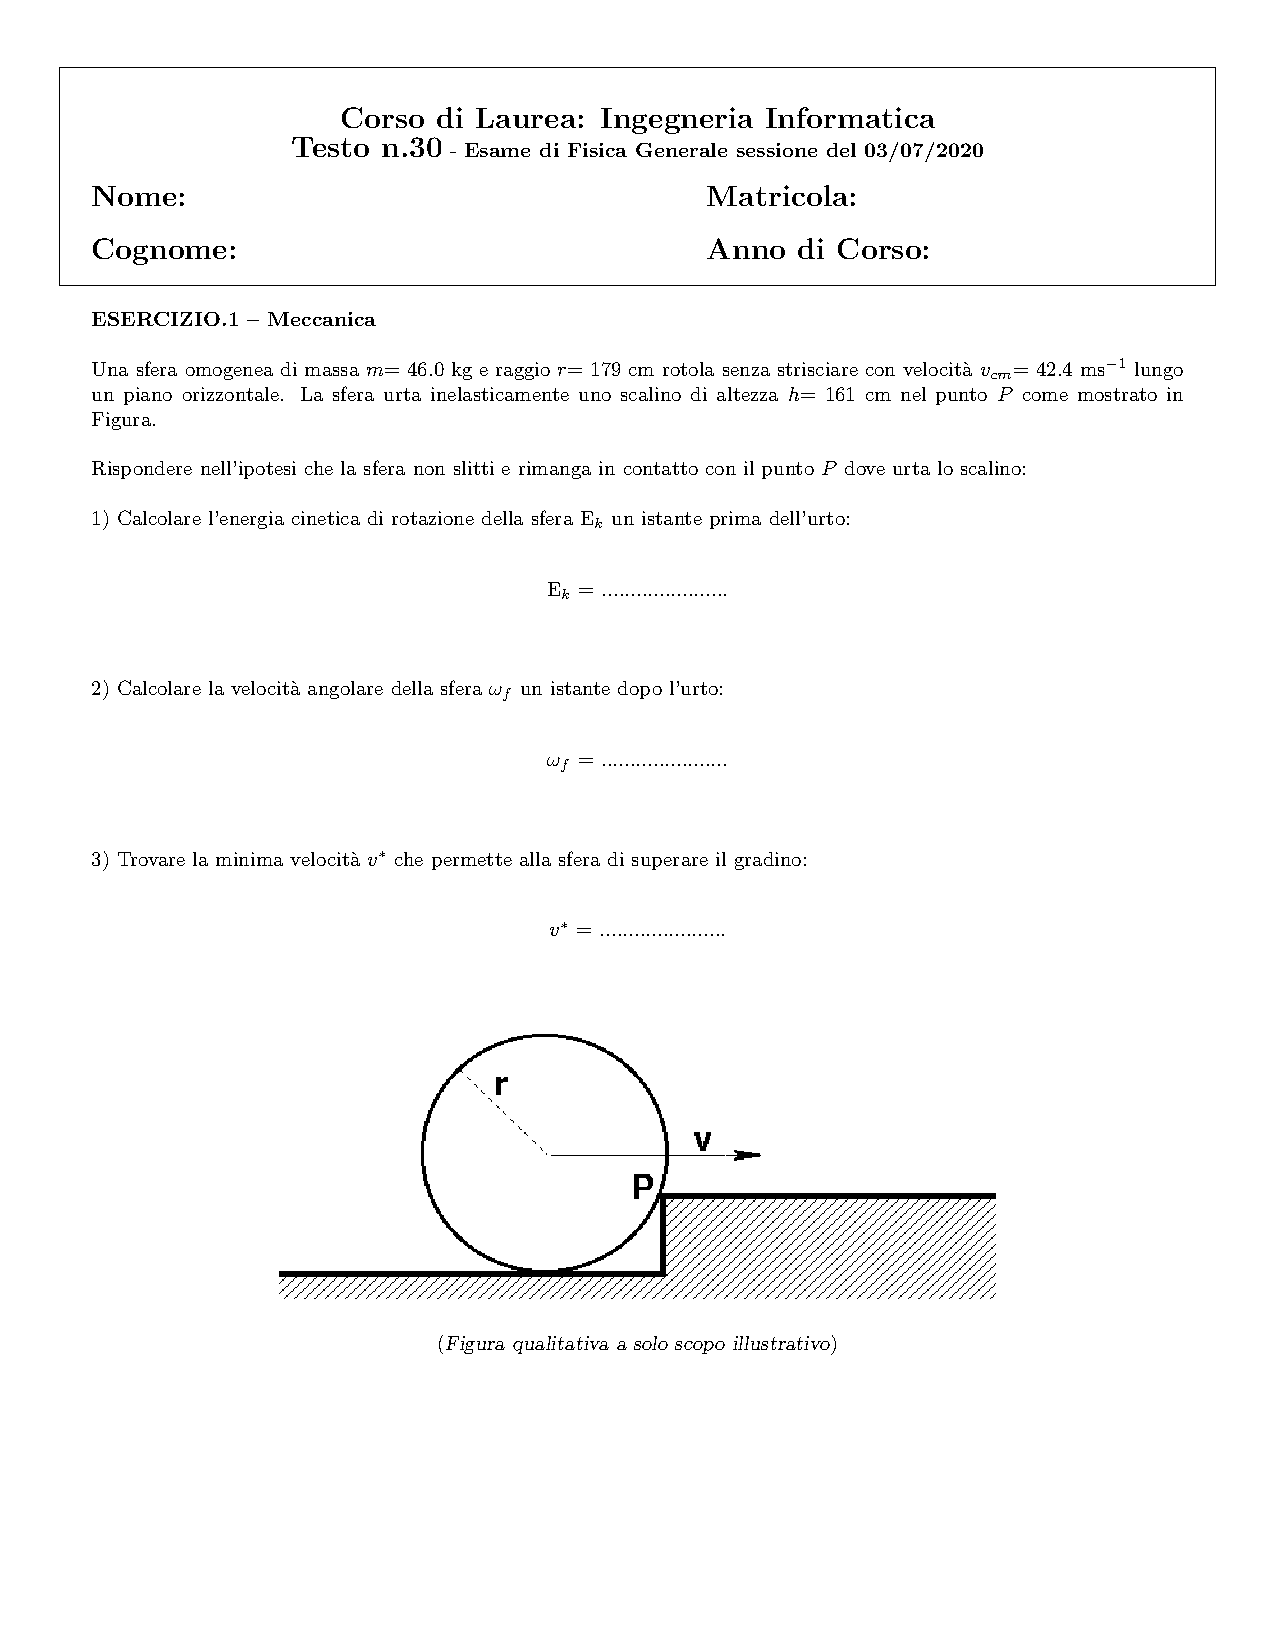
\includegraphics{img/30.PNG}
\end{center}
\subsection{ROTATE LEFT}
\begin{center}
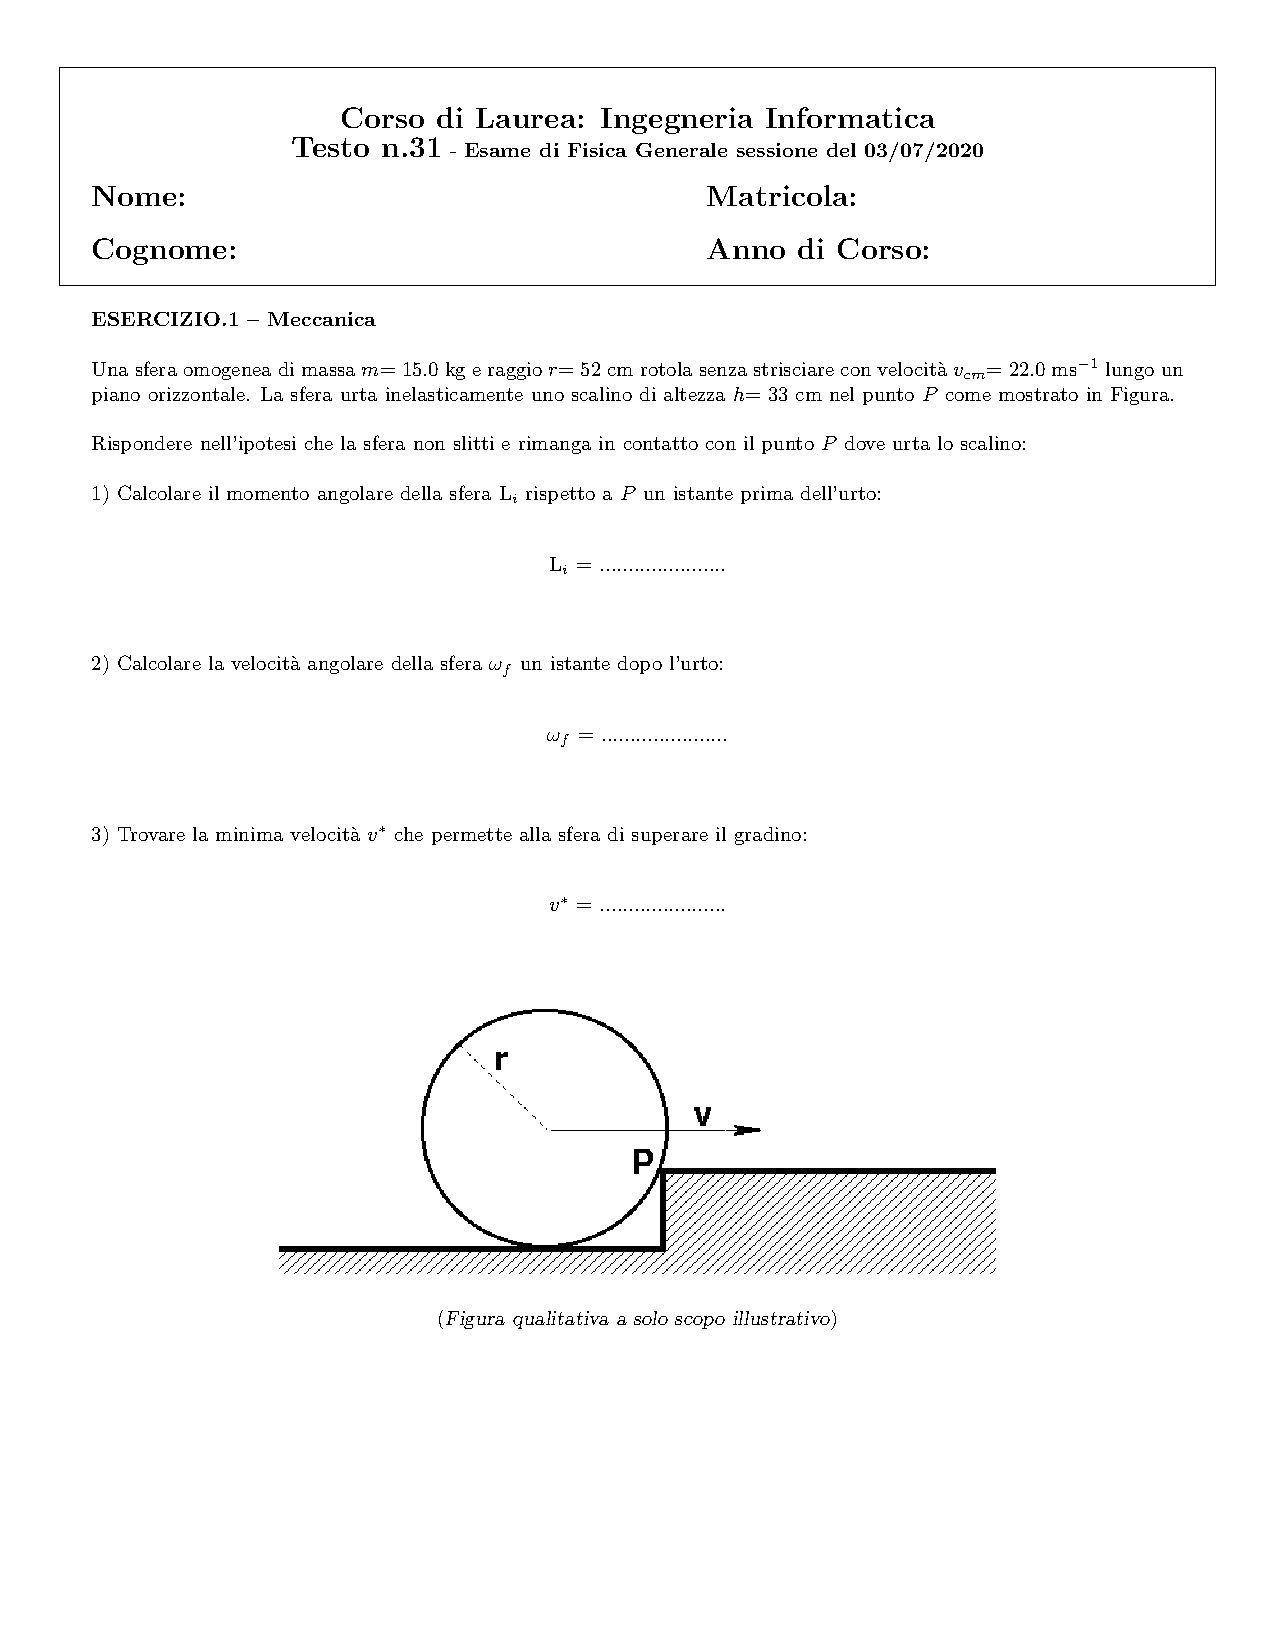
\includegraphics{img/31.PNG}
\end{center}

\clearpage

\section{Istruzioni logiche}
Le istruzioni logiche permettono l'applicazione degli operatori dell'\emph{Algebra di Boole}. Bisogna tenere conto di eventuali flag modificati (generalmente vengono modificati). Le seguenti operazioni applicano BIT a BIT le operazioni appena dette:

\subsection{NOT}
\begin{center}
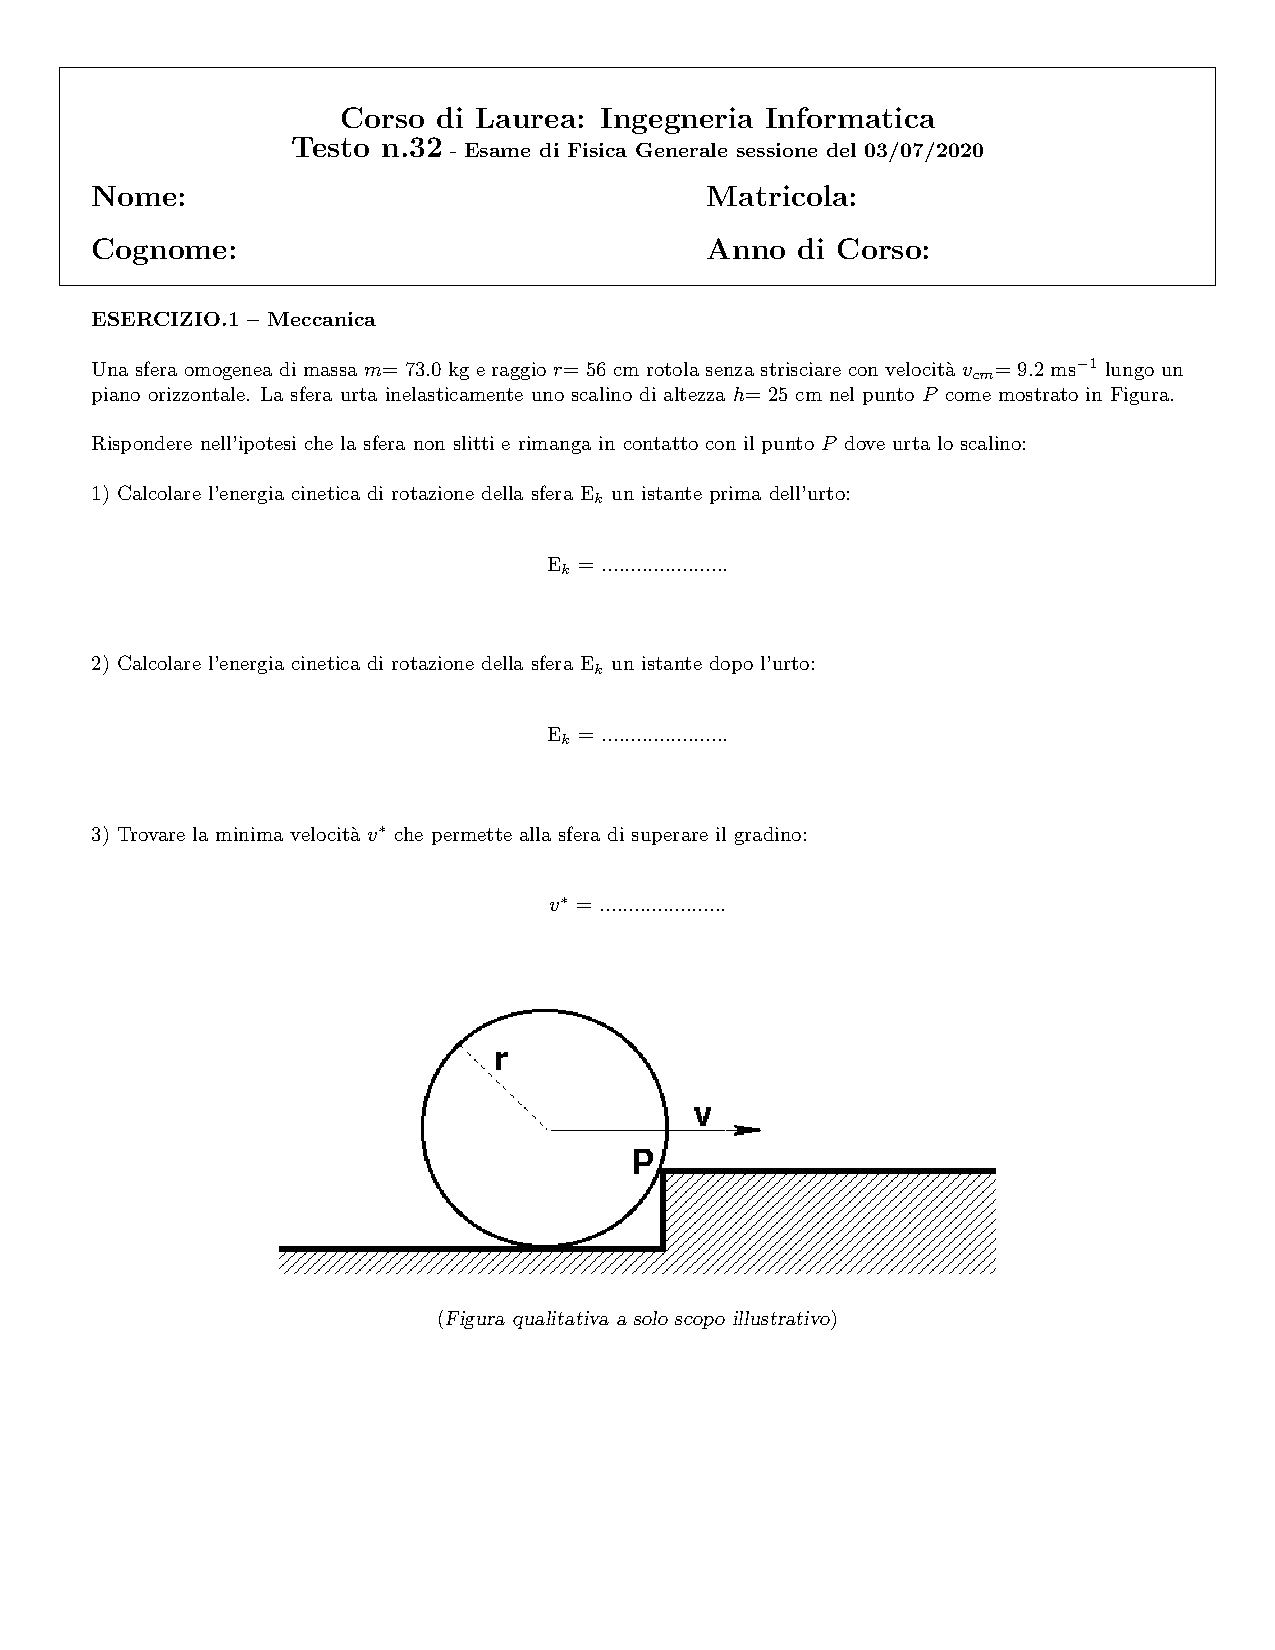
\includegraphics{img/32.PNG}
\end{center}
\subsection{AND}
\begin{center}
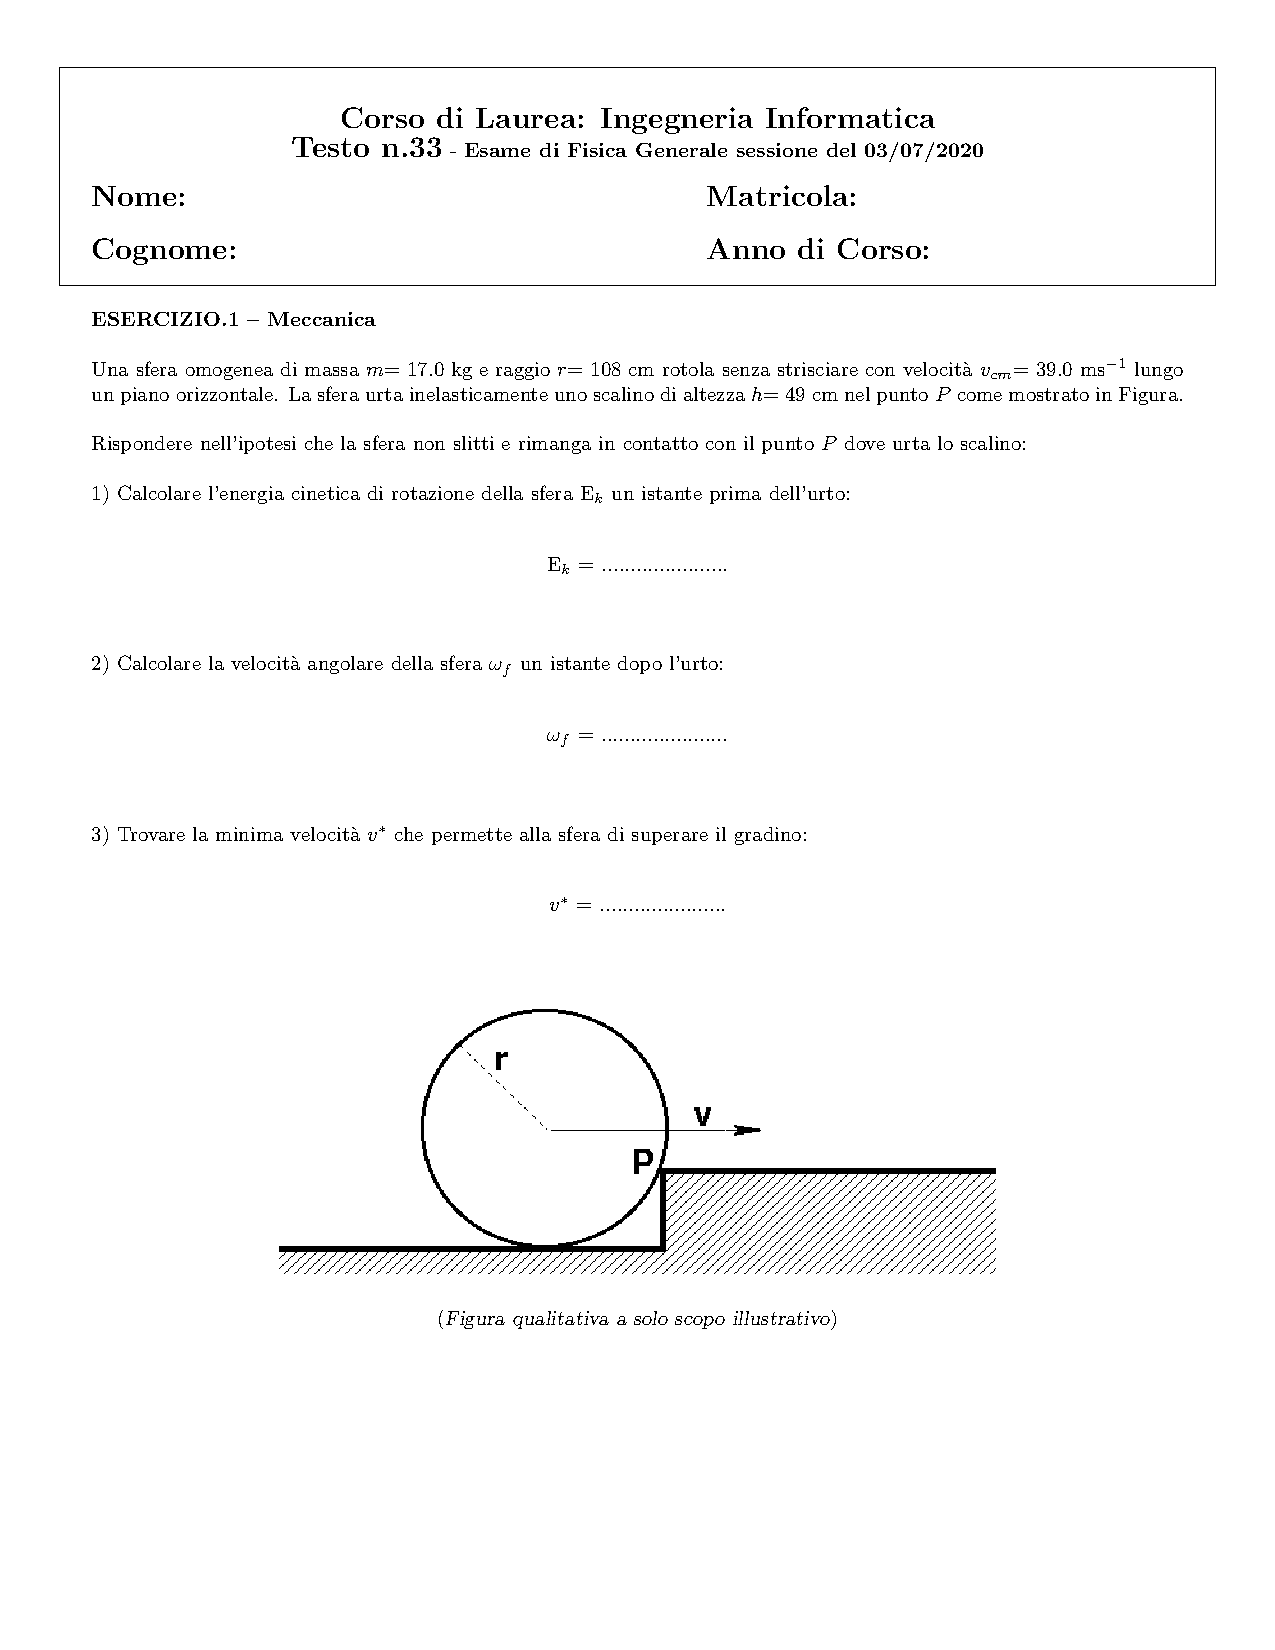
\includegraphics{img/33.PNG}
\end{center}
\subsection{OR}
\begin{center}
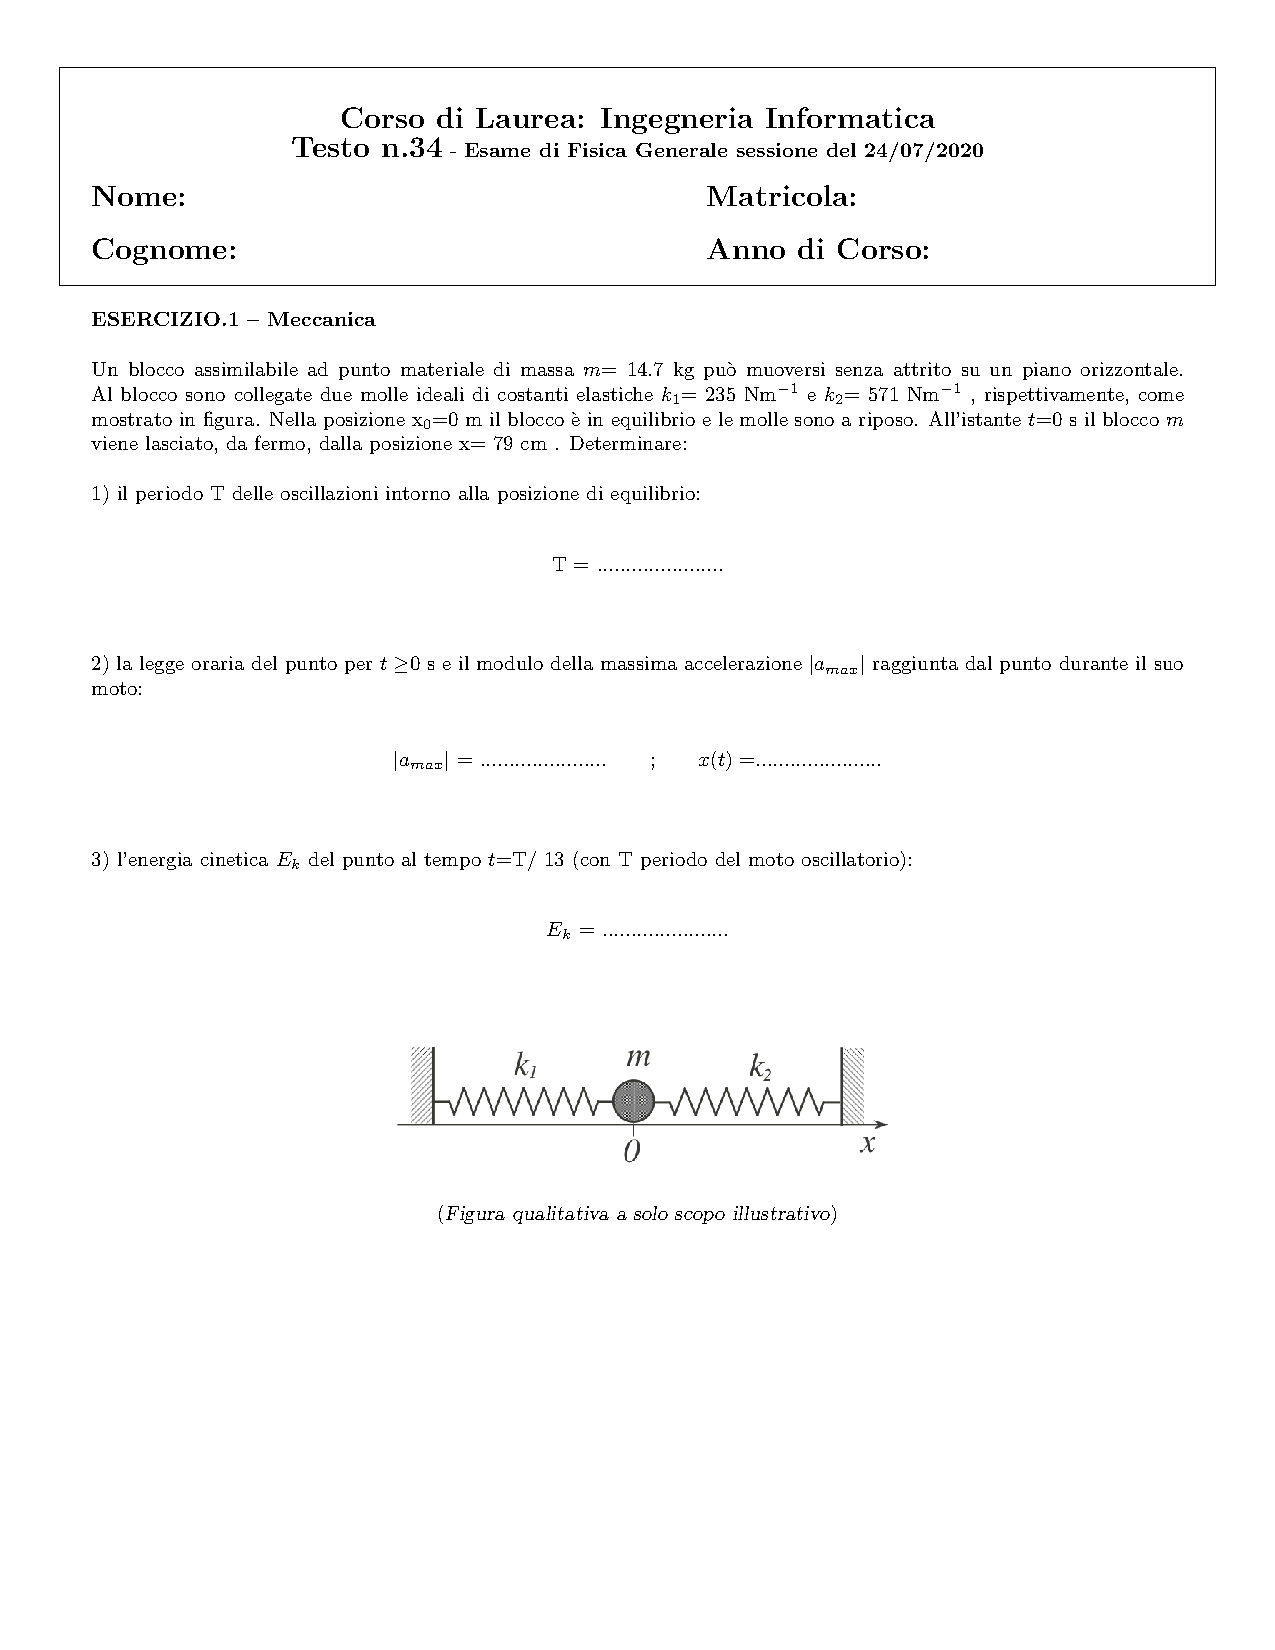
\includegraphics{img/34.PNG}
\end{center}
\subsection{XOR (OR esclusivo)}
\begin{center}
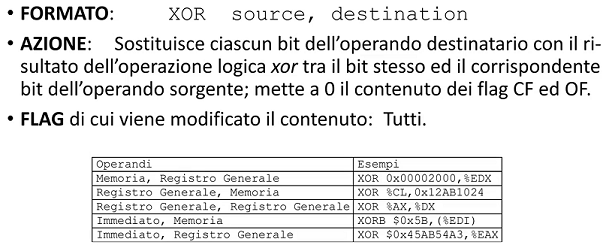
\includegraphics{img/35.PNG}
\end{center}
\subsection{Utilizzi di questi operatori}
\begin{itemize}
\item Singoli bit di un operando possono essere resettati usando l'operatore AND\\(usando una maschera formata da soli 1 tranne nel bit che si vuole resettare).
\item Singoli bit di un operando possono essere settati usando l'operatore OR\\(usando una maschera formata da soli 0 tranne nel bit che si vuole settare)
\item Singoli bit di un operando possono essere invertiti rispetto all'attuale valore usando l'operatore XOR (usando una maschera formata da soli 0 tranne nel bit che si vuole invertire). Ricordiamo che \[\alpha \text{ XOR } 0 = \alpha\,\,\,\,\,\,\alpha \text{ XOR } 1 = \overline{\alpha}\]
\item \textbf{Applicazioni pratiche}:
\begin{itemize}
\item L'operatore AND può essere usato per estendere operandi naturali. Supponiamo di voler sommare due numeri naturali: uno in AL e un altro in EBX. \begin{verbatim}
MOV $5, %AL
MOV $100000, %EBX
AND $0x000000FF, %EAX
ADD %EAX, %EBX
\end{verbatim}
\item XOR può essere usato per resettare un registro: uso la XOR (ponendo EAX sia come source che come dest) invece della MOV. 
\begin{verbatim}
XOR %EAX, %EAX
\end{verbatim}
Nel confronto bit a bit ho sempre due bit uguali, quindi ottengo 0 ogni volta! Ulteriore nota: la MOV, come istruzione, occupa maggiore spazio.
\end{itemize}
\end{itemize}
\clearpage

\section{Istruzioni di controllo}
Il flusso del programma normalmente è sequenziale: le istruzioni stanno in memoria consecutivamente e il processore, normalmente, incrementa EIP puntano l'area di memoria immediatamente successiva. Questa regola non vale più quando intervengono istruzioni di controllo: queste scrivono un nuovo valore in EIP alterando il normale flusso. Abbiamo due tipi di istruzioni:
\begin{itemize}
\item Istruzioni di salto (Jmp, Jcon). Nel salto non si memorizzano informazioni relative al punto da cui si è compiuto il salto (neanche implicitamente).
\item Istruzioni per la gestione di sottoprogrammi (CALL, RET). Si memorizzano informazioni relative al salto (attraverso la pila)
\end{itemize}

\subsection{JUMP}
\begin{center}
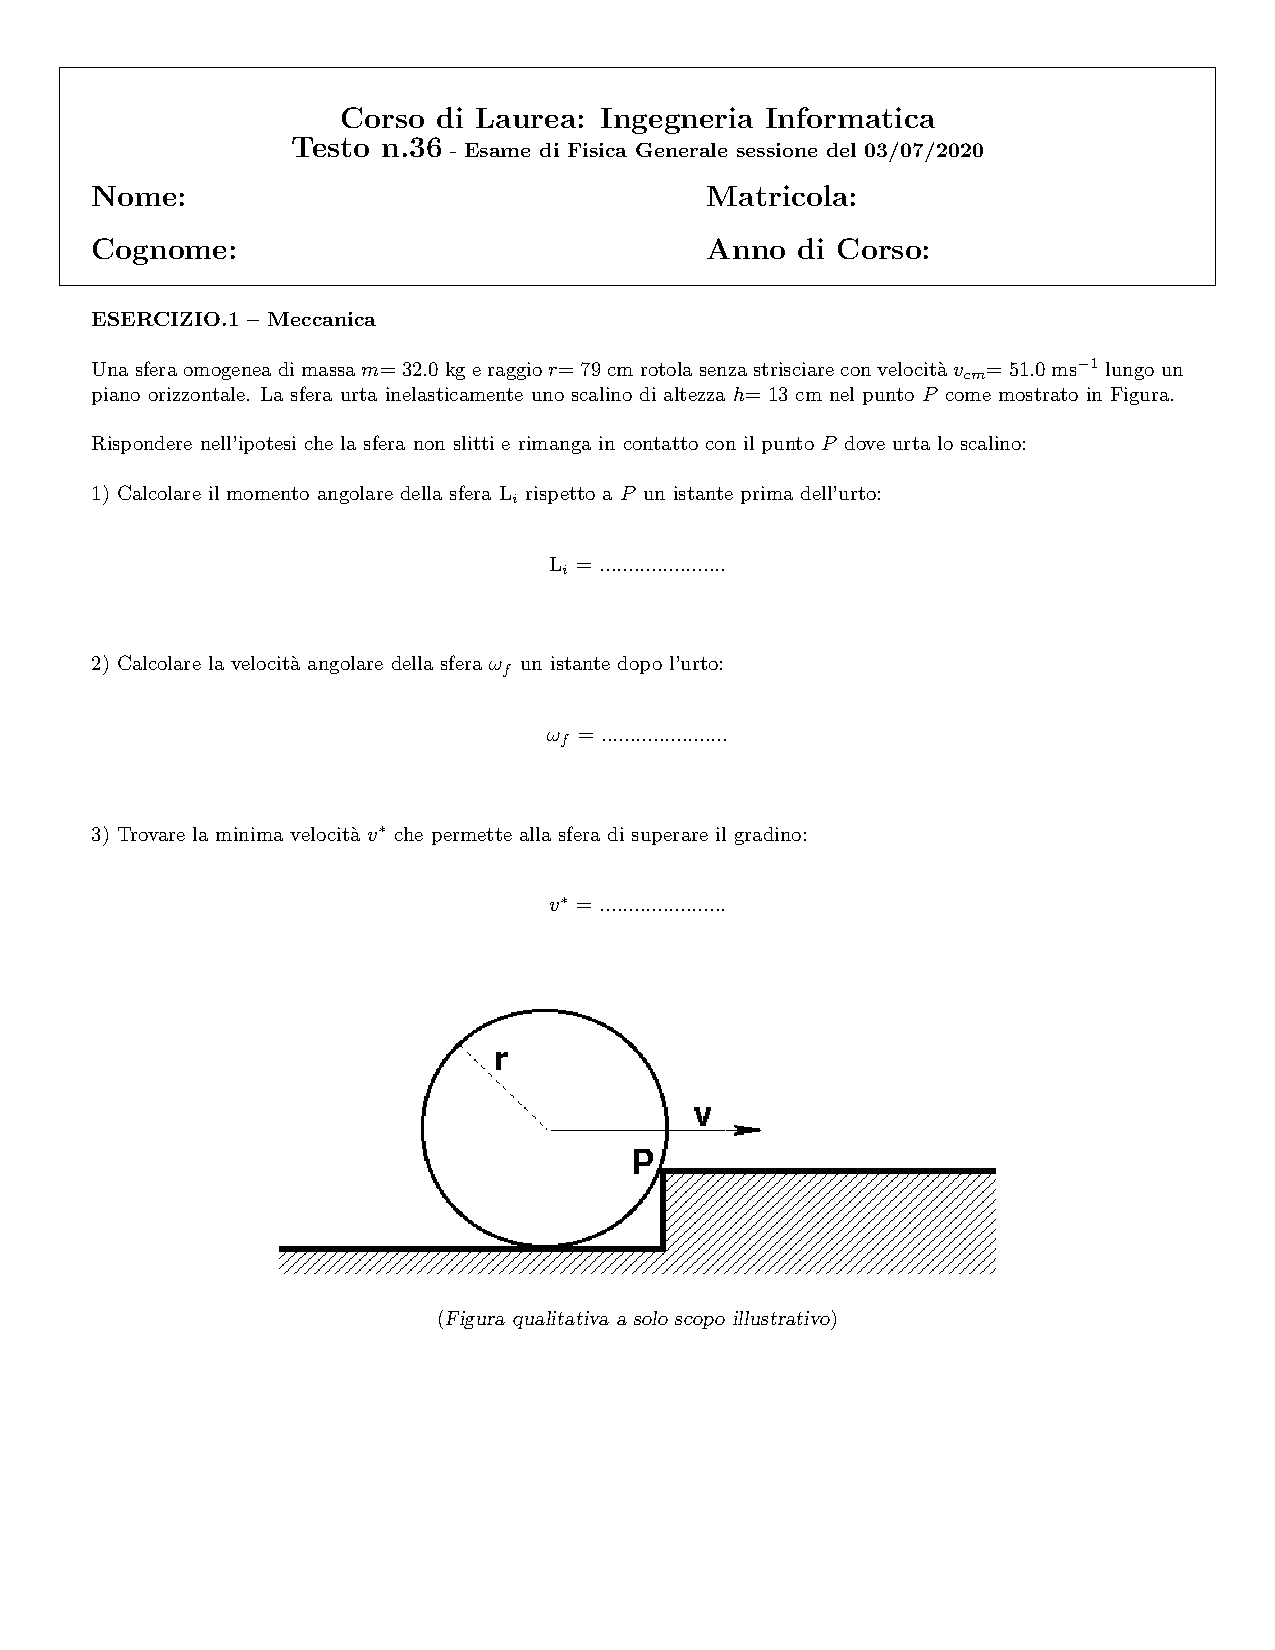
\includegraphics{img/36.PNG}
\end{center}

\subsection{JUMP if condition met}
\begin{center}
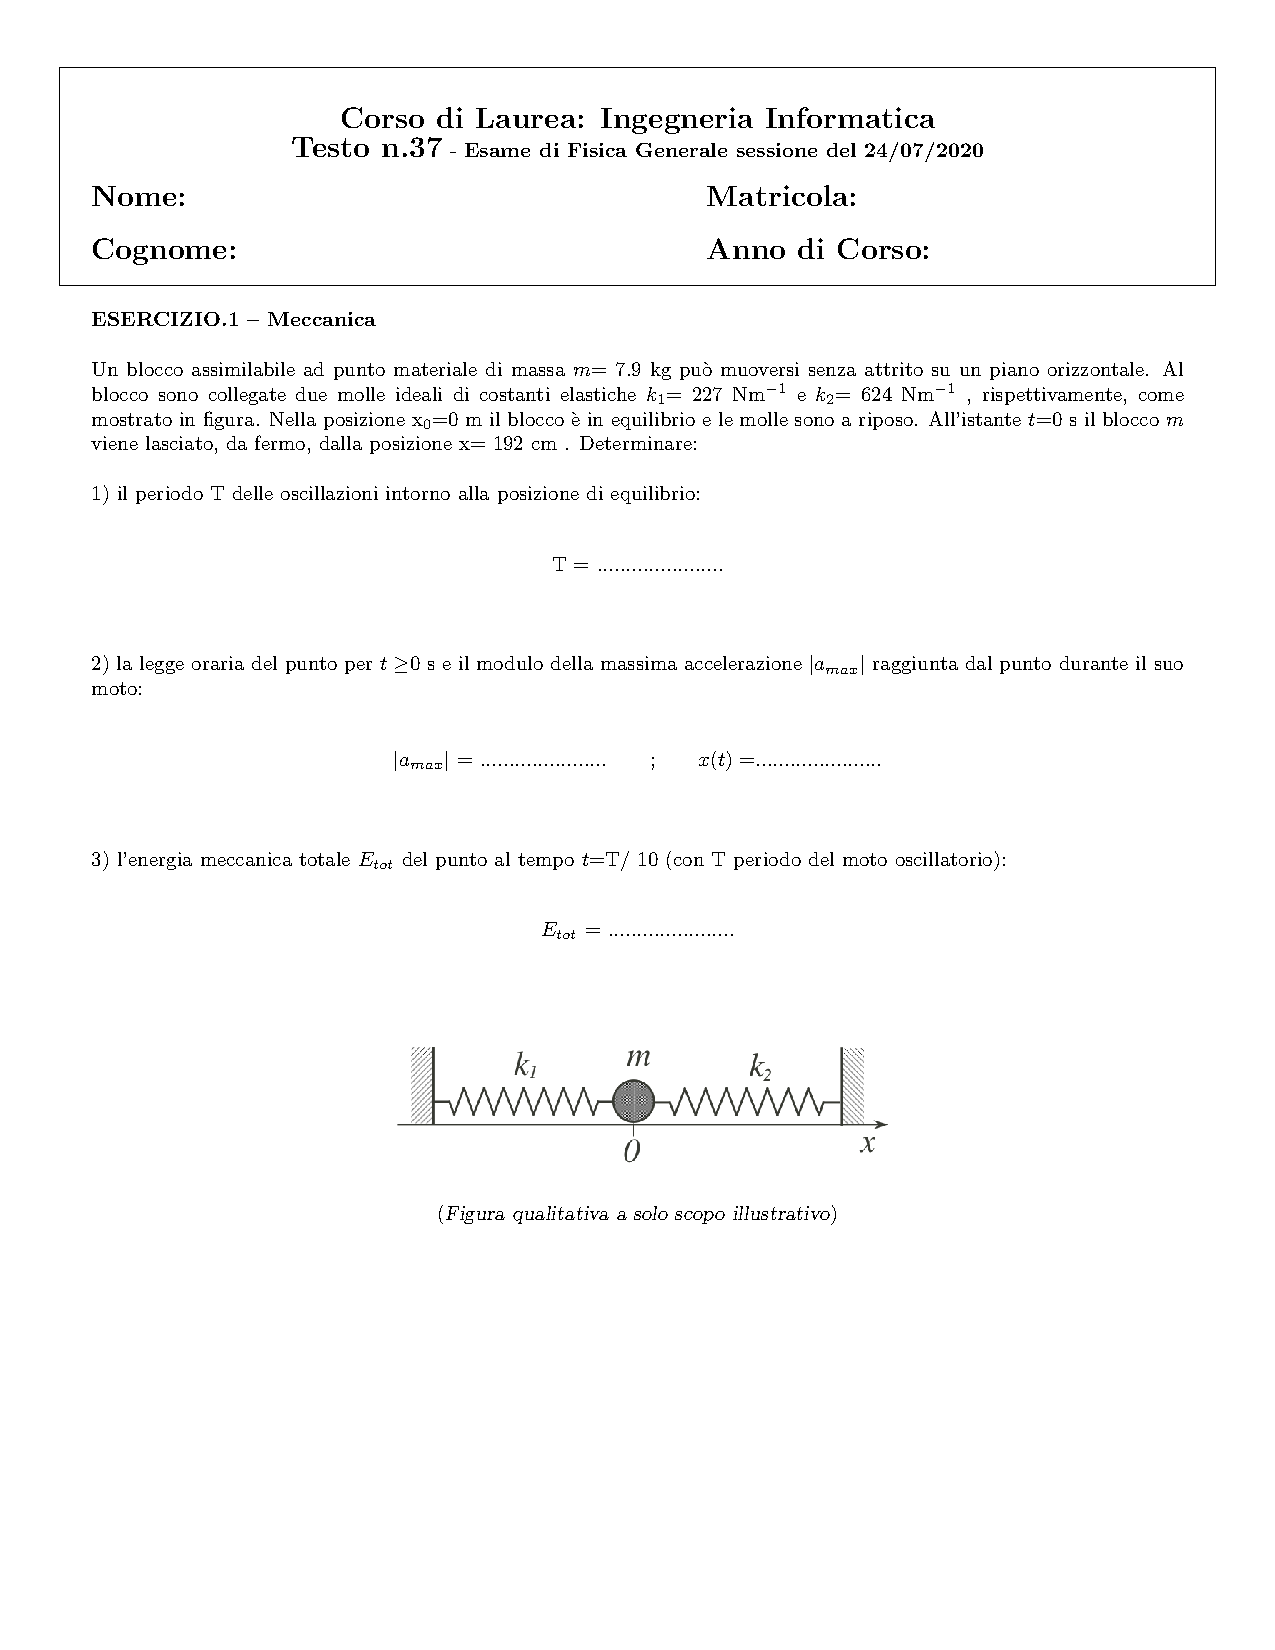
\includegraphics{img/37.PNG}
\end{center}
Tabella completa con le condizioni a pagina 22 del libro di Corsini.
\paragraph{Cose di cui tenere conto}
\begin{itemize}
\item Le JUMP condizionate si basano sui valori di certi flag, quindi vengono eseguite a seguito di CMP o operazioni aritmetiche.
\item Il soggetto è sempre l'operando destinatario: se io dico JA significa che voglio verificare se l'operando destinatario è maggior dell'operando sorgente (naturali).
\item Si distinguono:
\begin{itemize}
\item JUMP condizionate utilizzabili in qualunque caso (CMP, operazioni aritmetiche...);
\item JUMP condizionate utilizzabili solo a seguito di operazioni CMP, precisamente...
\begin{itemize}
\item JUMP per confronti tra numeri naturali (\emph{Above} e \emph{Below}), e
\item JUMP per confronti tra numeri interi (\emph{Greater} e \emph{Less}).
\end{itemize}
\end{itemize}
\end{itemize}

\subsection{Sottoprogrammi}
Le istruzioni coinvolte sono due:
\begin{itemize}
\item CALL, salto ad un sottoprogramma
\item RET, ritorno al programma chiamante
\end{itemize}
entrambe fanno riferimento, come già detto, alla pila.
\subsubsection{CALL}
\begin{center}
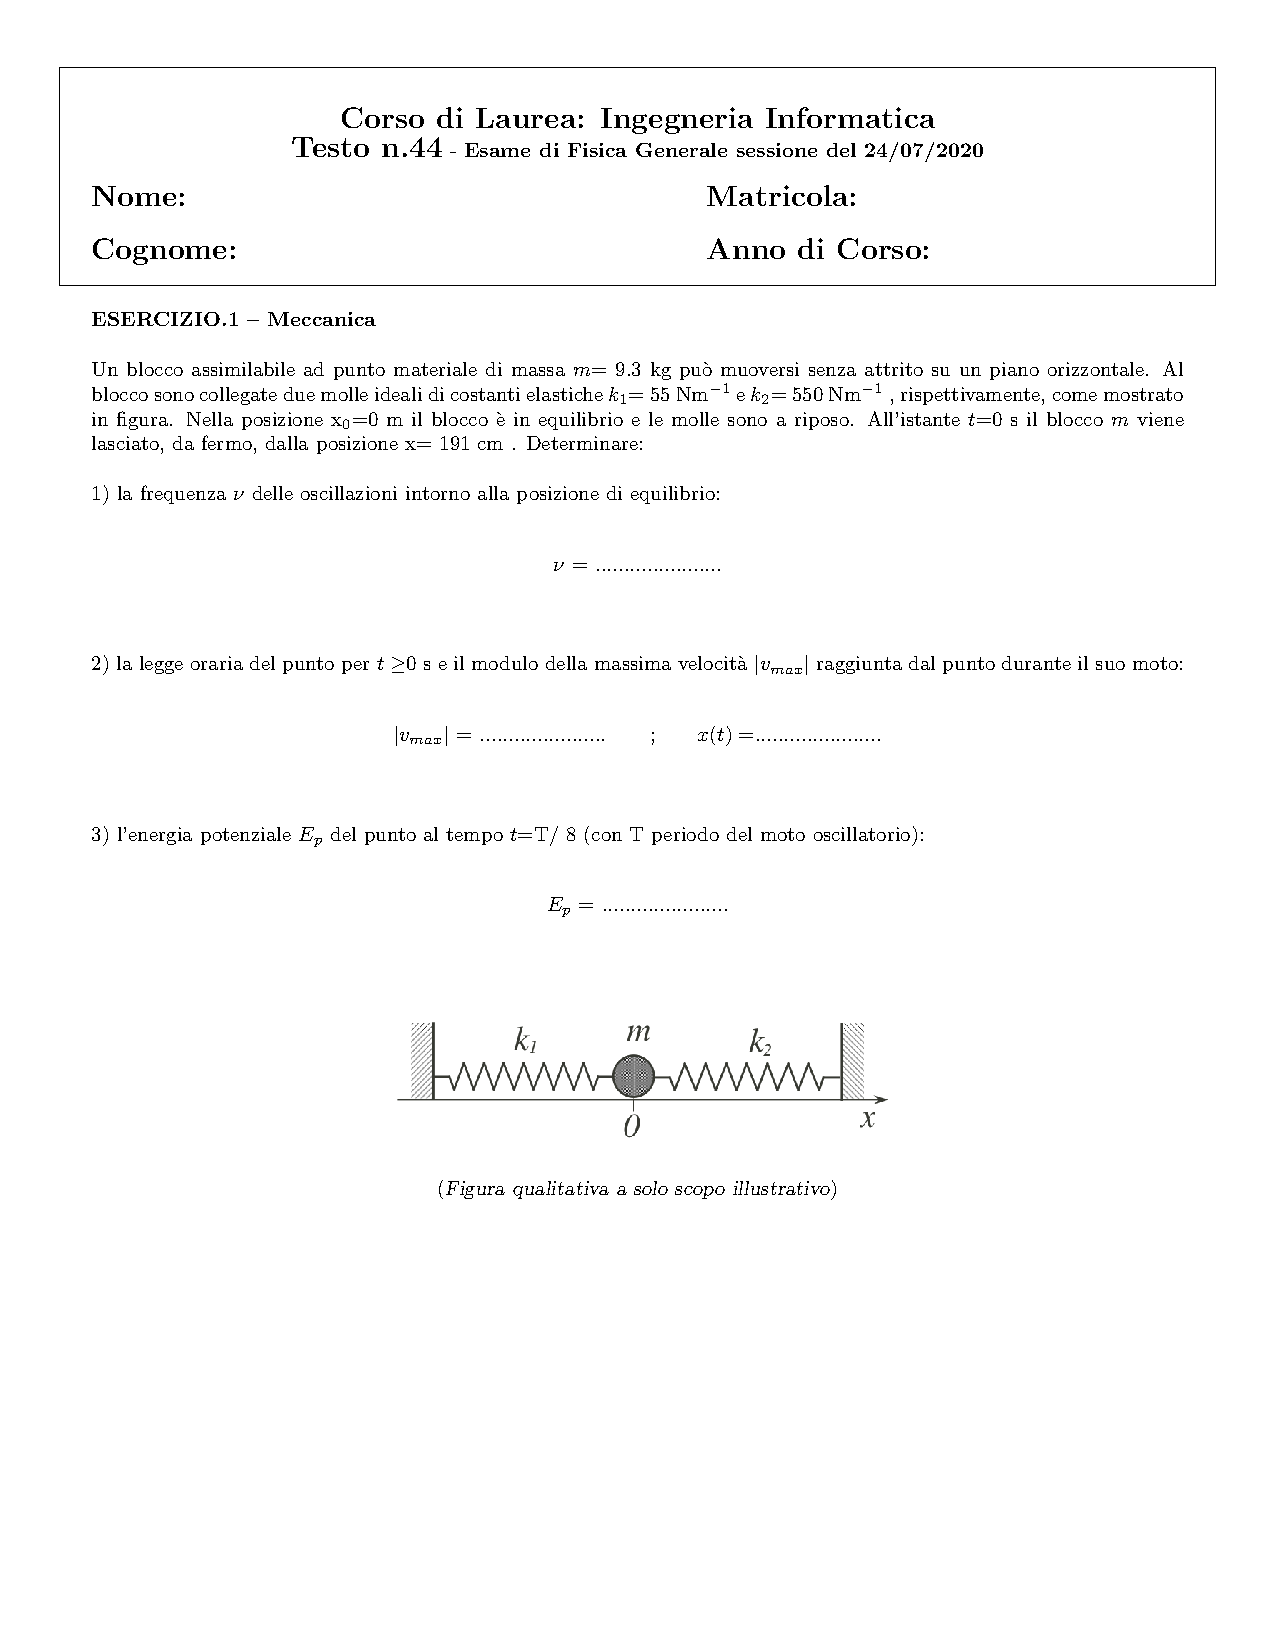
\includegraphics{img/44.PNG}
\end{center}
\subsubsection{RET}
\begin{center}

\includegraphics{img/45.PNG}
\end{center}
\subsubsection{NO OPERATION}
\begin{center}
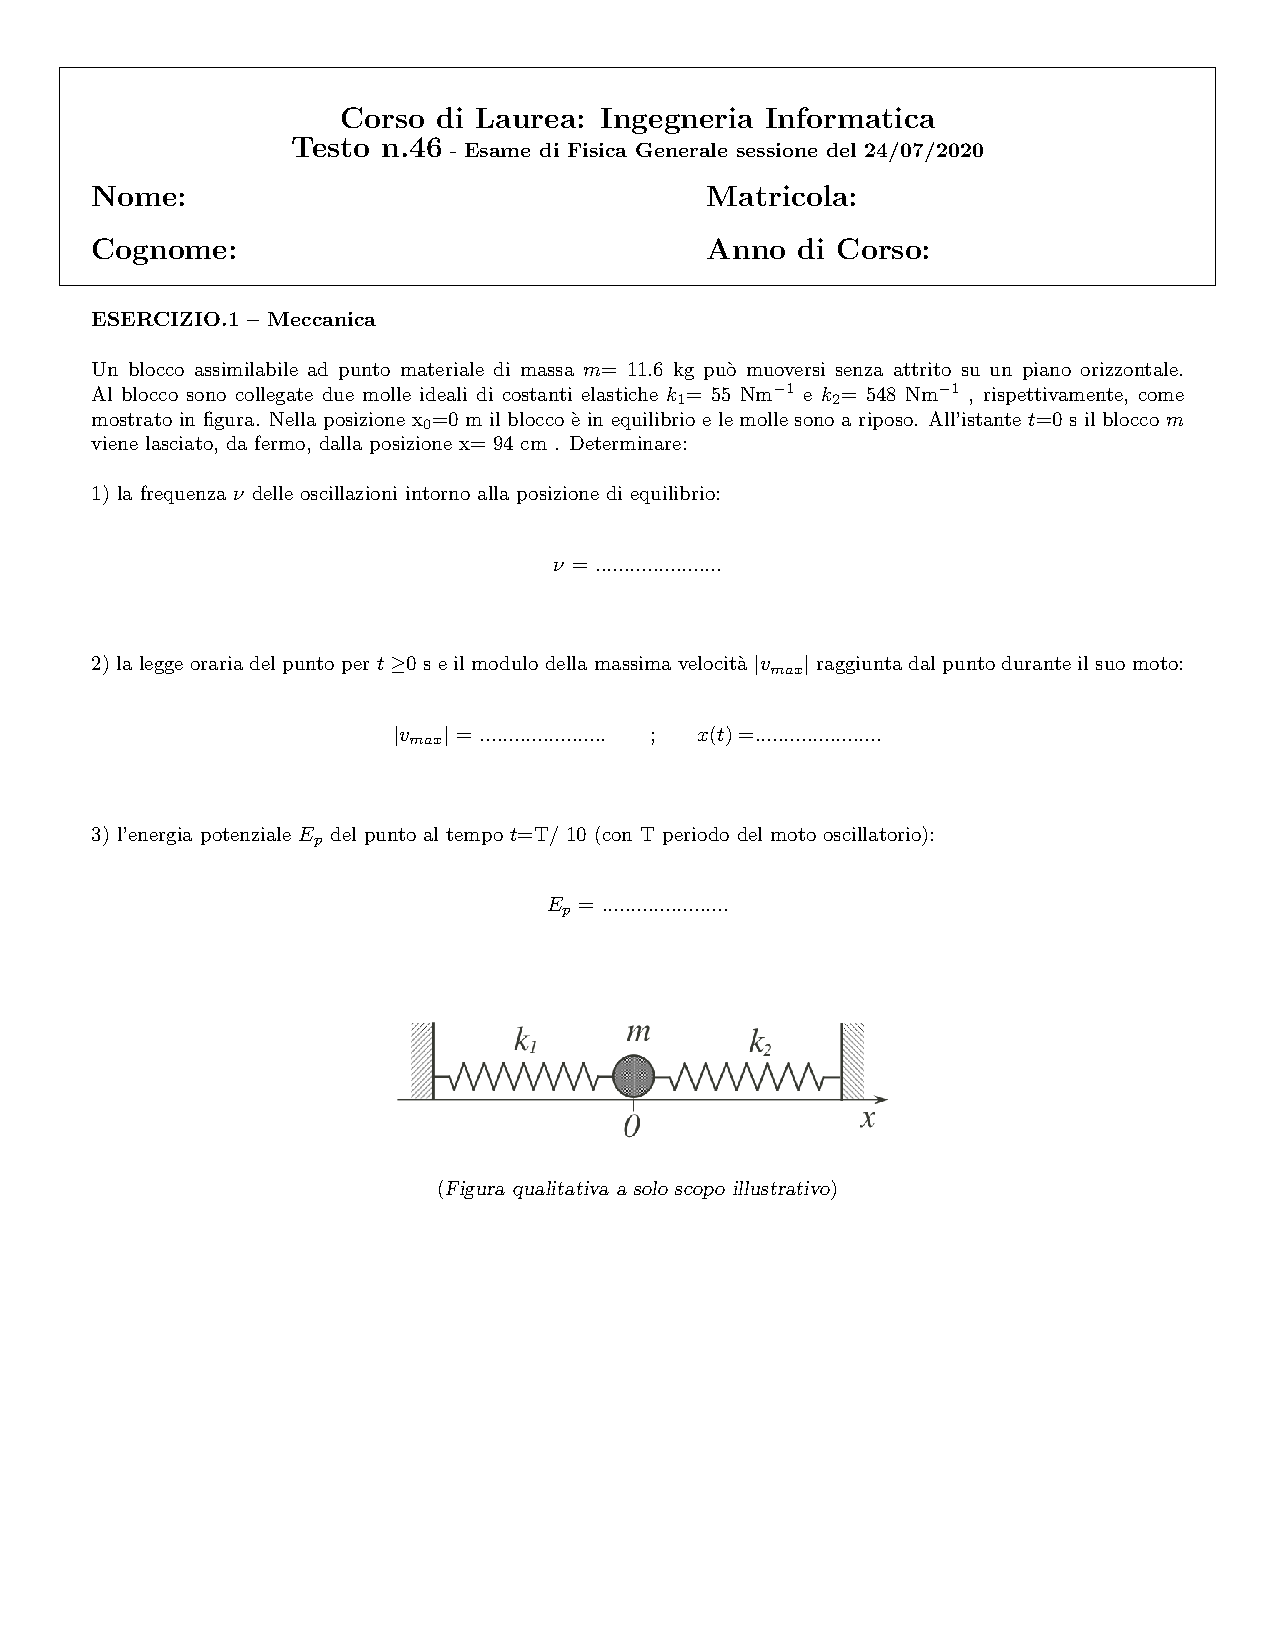
\includegraphics{img/46.PNG}
\end{center}
\subsubsection{HALT}
\begin{center}
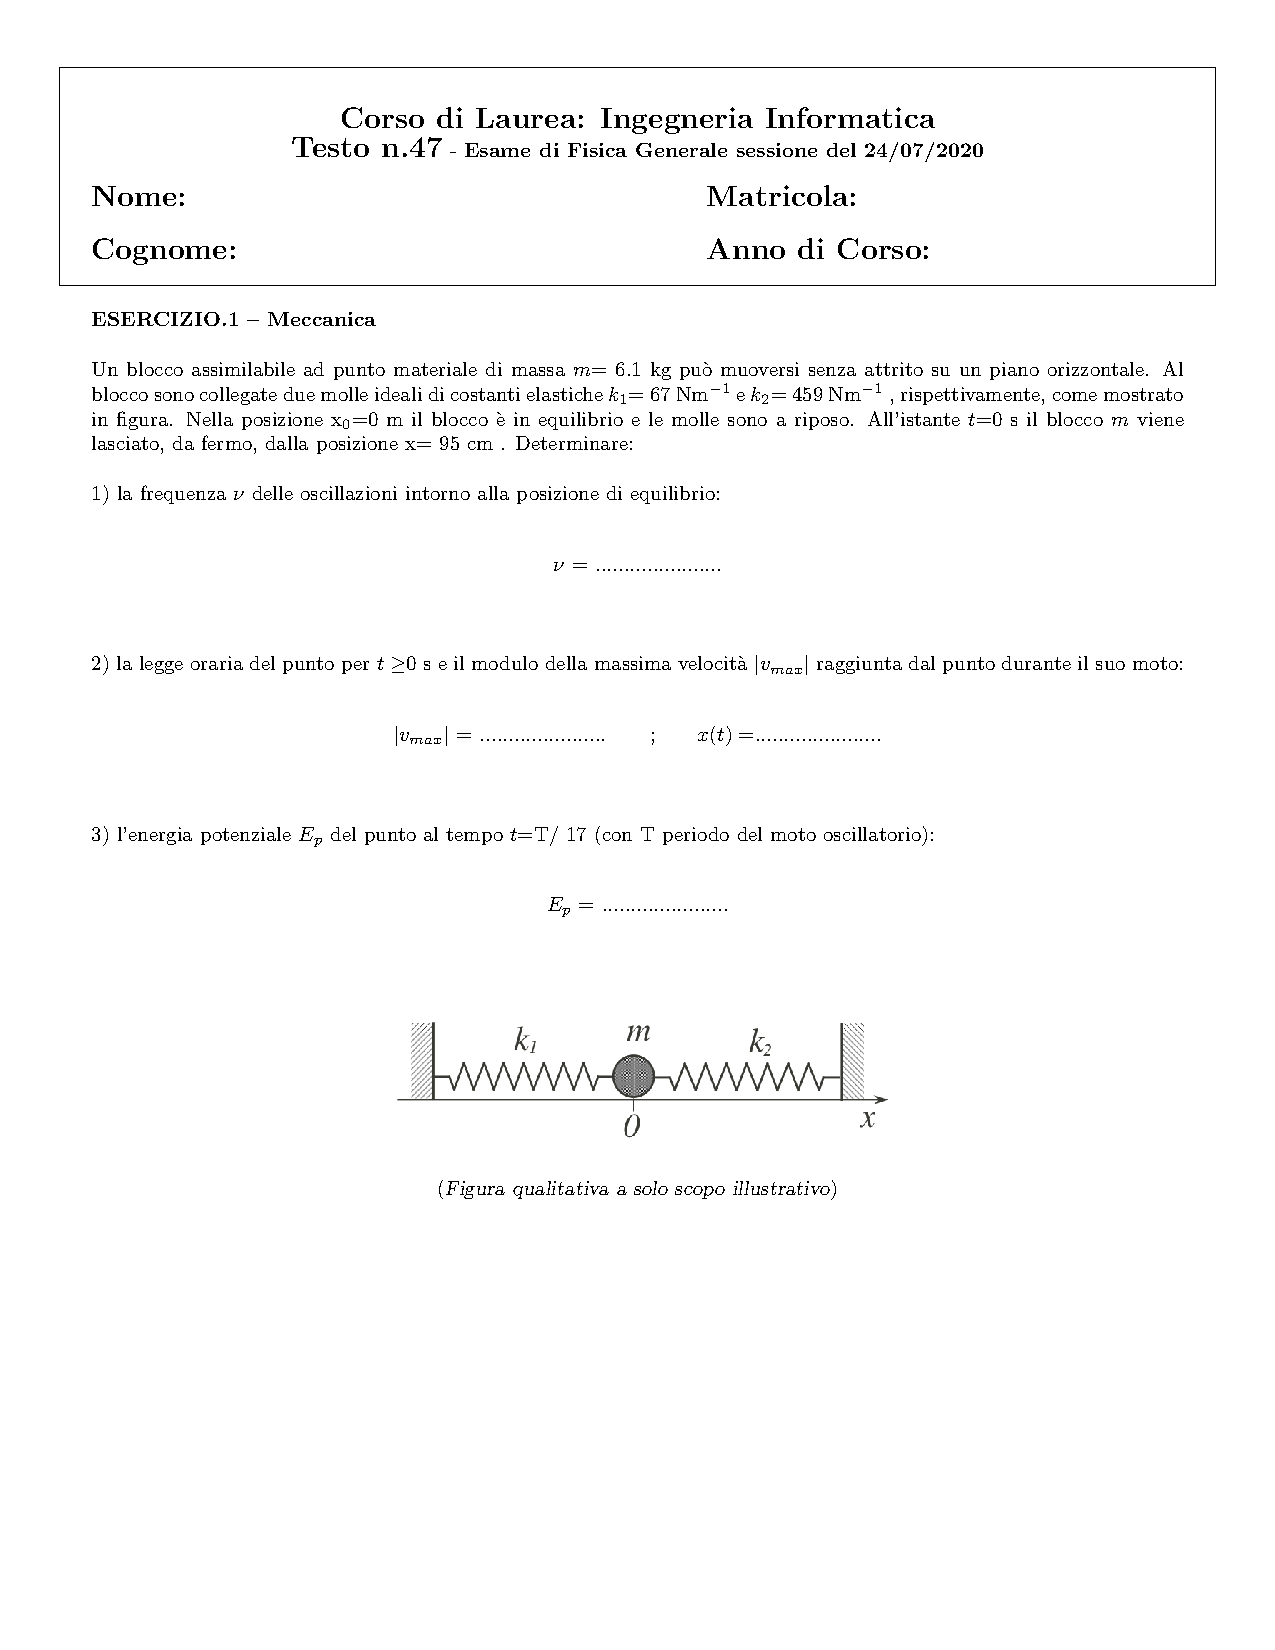
\includegraphics{img/47.PNG}
\end{center}
\section{Protezione ed istruzioni privilegiate}
\begin{itemize}
\item Il processore può funzionare in due modalità: utente e sistema. 
\item La modalità sistema permette l'esecuzione di tutte le istruzioni, la modalità utente permette l'esecuzione di una sola parte di queste istruzioni. 
\item Delle operazioni viste le seguenti sono istruzioni privilegiate non eseguibili in modalità utente: HLT, IN, OUT. Se chiamate va in esecuzione un'eccezione di protezione (comportamento diverso da sistema a sistema).
\end{itemize}
\paragraph{Relativamente all'I/0} Faremo IN e OUT attraverso sottoprogrammi di servizio (li vedremo più avanti). IN e OUT sono istruzioni privilegiate poichè è facile portarle in stato inconsistente.

\clearpage
\section{Flag controllati dalle istruzioni condizionate}
Si tenga conto che il soggetto delle condizioni è sempre l'operando destinatario.
\begin{itemize}
\item \textbf{Equal}: $\text{ZF}=1$
\item \textbf{Not equal}: $\text{ZF}=0$
\item Naturali:
\begin{itemize}
\item \textbf{Above}: $\text{CF}=0$, $\text{ZF}=0$
\item \textbf{Above or equal}: $\text{CF}=0$
\item \textbf{Below}: $\text{CF}=1$
\item \textbf{Below or equal}: $\text{CF}=1$ o $\text{ZF}=1$
\end{itemize}
\item Interi:
\begin{itemize}
\item \textbf{Greater}: $\text{ZF}=0$, $\text{SF}=\text{OF}$
\item \textbf{Greater or equal}: $\text{SF}=\text{OF}$
\item \textbf{Less}: $\text{SF} \neq \text{OF}$
\item \textbf{Less or equal}:  $\text{SF} \neq \text{OF}$ o  $\text{ZF}=1$
\end{itemize}
\item \textbf{Zero}: $\text{ZF}=1$. Il risultato dell'operazione precedente è stato uguale a zero.
\item \textbf{Not zero}: $\text{ZF}=0$. Il risultato dell'operazione precedente è stato diverso a zero.
\item \textbf{Carry}: $\text{CF}=1$
\item \textbf{No Carry}: $\text{CF}=0$
\item \textbf{Overflow}: $\text{OF}=1$
\item \textbf{No Overflow}: $\text{OF}=0$
\item \textbf{Sign}: $\text{ZF}=1$
\item \textbf{No Sign}: $\text{ZF}=0$
\end{itemize}
\paragraph{Perchè si guarda l'overflow per le condizioni riguardo gli interi?} Bisogna considerare sia il caso senza overflow che quello senza. Si consideri che il segno del risultato della sottrazione sarà sbagliato in caso di overflow, quindi dobbiamo verificare che il suo valore sia l'opposto di quello previsto.
\begin{itemize}
\item in \textbf{Greater or equal}: mi aspetto una differenza con segno positivo. Se non ho l'overflow avrò $\text{SF}=\text{OF}= 0$. Se ho l'overflow avrò $\text{OF}= 1$. Se il valore del segno deve essere l'opposto di quello previsto dovrò avere  $\text{SF}=1$, quindi $\text{SF}=\text{OF}= 1$.
\item in \textbf{Less or equal}: mi aspetto una differenza con segno negativo. Se non ho l'overflow avrò $\text{SF}=1$ e $\text{OF}=0$. Se ho l'overflow avrò $\text{OF}= 1$. Se il valore del segno deve essere l'opposto di quello previsto dovrò avere  $\text{SF}=0$, quindi $\text{SF}=0$, $\text{OF}= 1$.
\end{itemize}
\chapter{Martedì 06/10/2020}

\section{Assemblatore} 
Utilizzeremo l'assemblatore \textbf{GAS} (\emph{GNU Assembler}): le informazioni per scaricarlo sono presenti sul sito del docente. Si raccomanda massimo rispetto della procedura di installazione.
\section{Struttura di un programma assembler}
Un programma Assembler si articolo in due sezioni:
\begin{itemize}
\item Sezione dati. Contiene le dichiarazioni delle variabili, cioè nomi simbolici per indirizzi di memoria.
\item Sezione codice. Istruzioni del programma
\end{itemize}
\paragraph{Direttive e istruzioni} In un programma sono presenti \textbf{direttive} (per esempio le dichiarazioni di variabili o di costanti) e \textbf{istruzioni} (ciò di cui abbiamo parlato fin dalla prima lezione). Ciascuna istruzione e direttiva è contenuta in una riga: alla fine è sempre presente il ritorno carrello \emph{CR} (anche nell'ultima riga di tutto il codice). In un codice ASS individueremo, in conclusione:
\begin{itemize}
\item Una prima parte contenente le direttive
\begin{verbatim}
.GLOBAL _main

.DATA
....
\end{verbatim}
la prima istruzione ci permette di stabilire quale sottoprogramma eseguire quando viene avviato l'applicativo. Nell'area .DATA indicheremo, come già detto, le variabili da utilizzare.
\item Una parte contenente le istruzioni
\begin{verbatim}
.TEXT
_main : NOP
        ...
        RET
\end{verbatim}
la RET deve essere posta in fondo ad ogni sottoprogramma, incluso quello principale. Relativamente alla NOP capiremo più avanti l'utilità nel porla all'inizio del sottoprogramma.
\end{itemize}
\paragraph{Ordine degli elementi} L'ordine degli elementi descritto non è l'unico possibile: quanto detto è consigliato per ottenere un programma leggibile.
\subsection{Assembler case-sensitive o case-insensitive?}
Assembler è:
\begin{itemize}
\item \textbf{case-insensitive} relativamente ai caratteri delle keyword. Si consiglia di porle in stampatello maiuscolo
\item \textbf{case-sensitive} relativamente alle etichette (nomi di variabili e nomi di sottoprogrammi). Significa che
\[\_\text{main} \neq \_\text{Main}\]
\end{itemize}

\subsection{Cosa cambia rispetto agli esempi di programmi visti in passato?}
\begin{center}
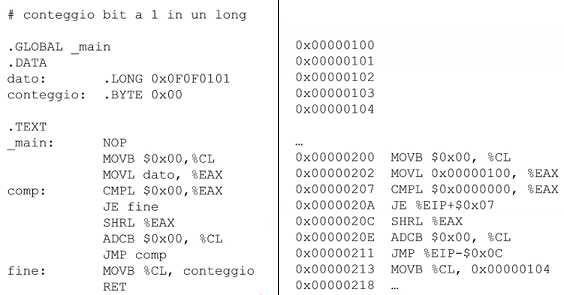
\includegraphics{img/48.PNG}
\end{center}
Il codice risulta decisamente più ordinato ma soprattutto andrò a richiamare aree di memoria usando nomi simbolici (e non più solo displacement). Queste etichette, che poniamo nella parte DATA, rappresentano simbolicamente l'indirizzo di quell'area di memoria. La cosa ci semplifica la vita non poco: le cose viste nelle lezioni precedenti saranno gestione dell'assemblatore.

\subsubsection{Attenzione al jump : confronto col C++}
Si individua nel codice richiami ad etichette dichiarate più avanti: questa cosa è impensabile in C++ ma possibile in Assembler. Questo perchè l'assemblatore
\begin{enumerate}
\item Controlla tutti i nomi
\item traduce
\end{enumerate}
l'approccio è necessario per poter svolgere salti in avanti, ma può essere anche mortale. Assembler, a differenze del C++, offre maggiori spazi di libertà: dobbiamo usare questi spazi con estrema cautela. Il suggerimento, in generale, è di continuare a rispettare la prassi del C++ (unica eccezione i salti in avanti). 
\paragraph{Altro esempio di porcheria} La libertà fornita da Assembler potrebbe portarci a scrivere quanto segue
\begin{verbatim}
nome1: 
nome2: CMP
        ...
        ...
        JMP nome1
        JMP nome2
\end{verbatim}
queste cose, pur essendo valide (di fatto abbiamo creato due alias per un sottoprogramma), sono porcherie da evitare.
\subsection{Riga di codice}
Le righe di codice presentano la seguente struttura
\begin{verbatim}
nome: KEYWORD operandi #commento [/CR]
\end{verbatim}
l'unico elemento obbligatorio in una riga è il carattere di ritorno carrello.

\section{Direttive}
\paragraph{Attenzione} Ricordarselo come l'ave maria
\[\boxed{\text{Direttive} \neq \text{Istruzioni}}\]
Le direttive presentano la seguente struttura
\begin{verbatim}
.KEYWORD operandi [\CR]
\end{verbatim}
\subsection{Dichiarazione di variabili}
Abbiamo già detto che dichiareremo variabili all'inizio del nostro programma. La cosa è utile non tanto per dire ad assembler su cosa stiamo lavorando ma per stabilire in modo agile quanta memoria ci serve. I tipi di variabili possibili sono:
\begin{itemize}
\item .WORD (2byte, 16bit)
\item .BYTE (1byte, 8bit)
\item .LONG (4byte, 32bit)
\end{itemize}
\begin{center}
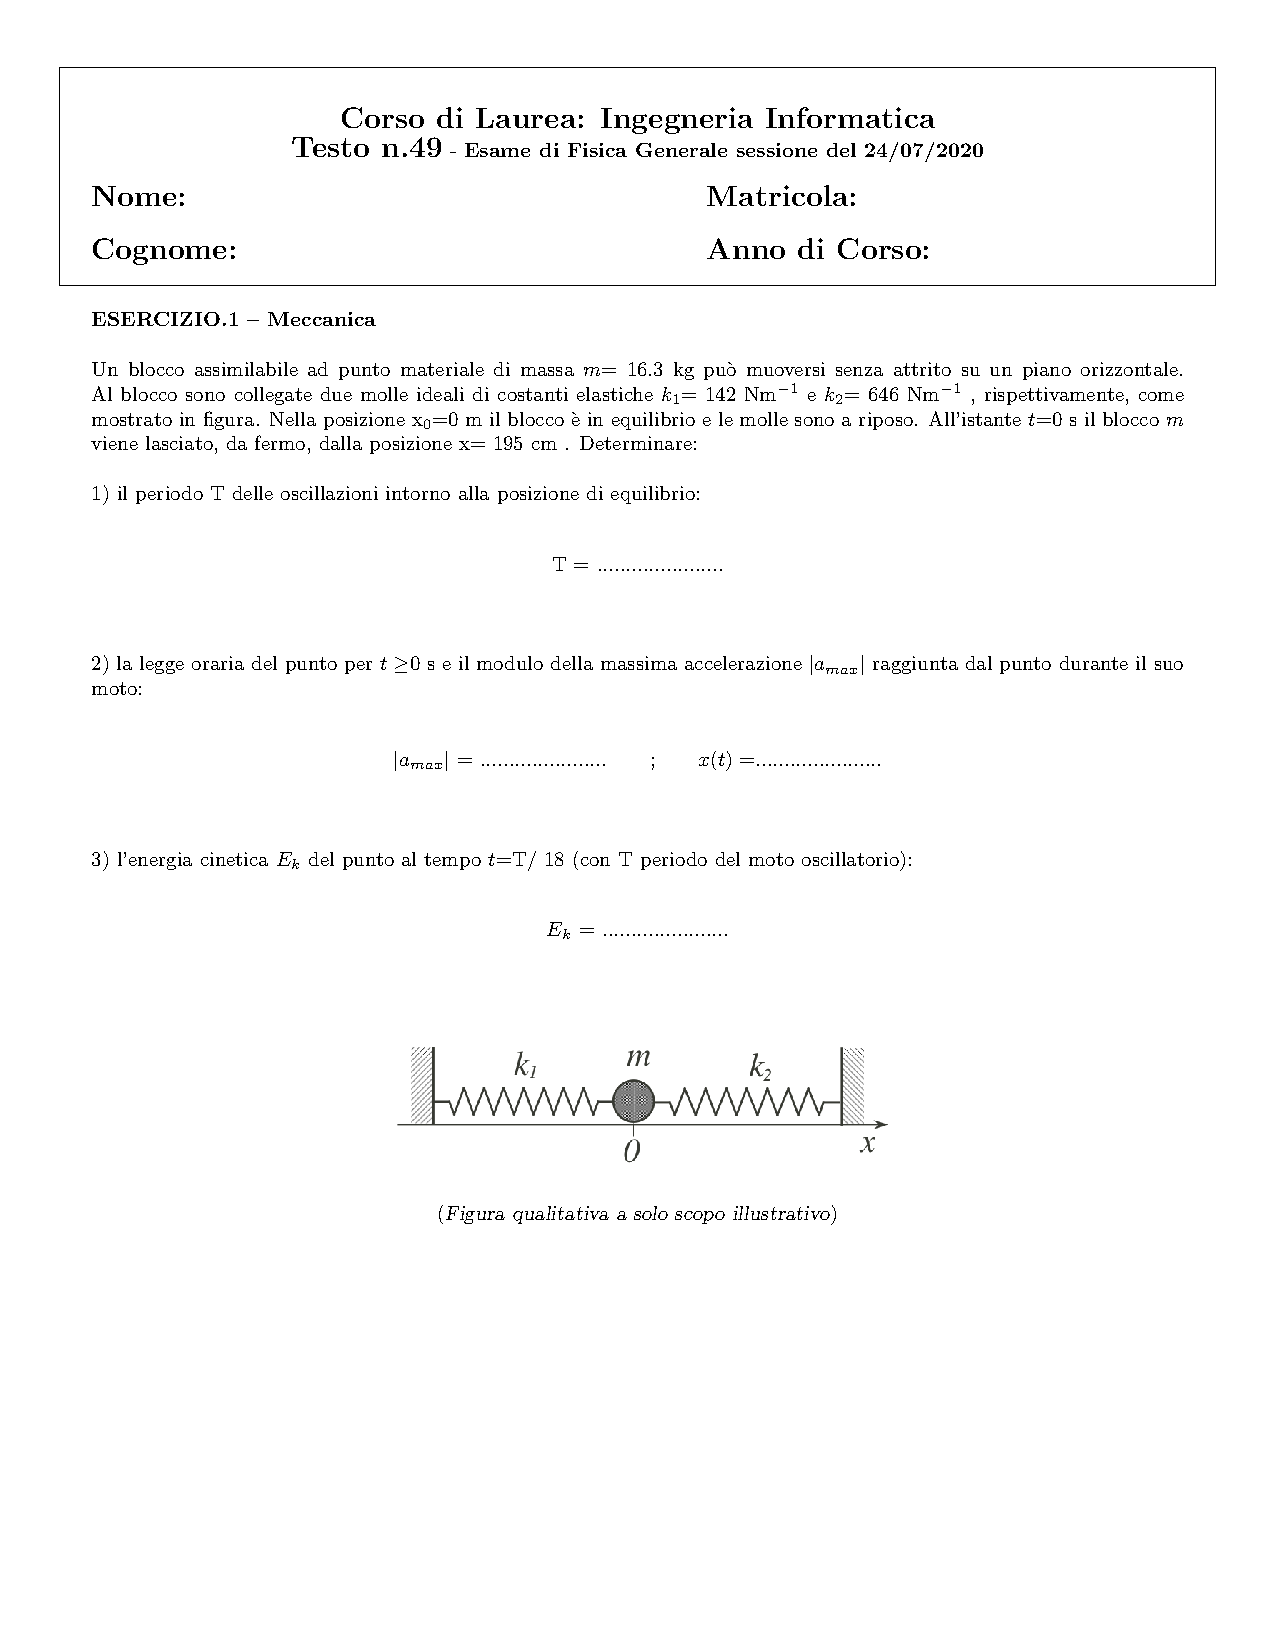
\includegraphics{img/49.PNG}
\end{center}
Individuiamo che
\begin{itemize}
\item è ammesso dichiarare variabili senza inizializzarle. Formalmente il valore inizializzato dovrebbe essere quello indicato in var0, ma la cosa non è certa e il comportamento della macchina imprevedibile. Si consiglia di inizializzare in qualunque caso
\item possiamo dichiarare variabili scalari, ma anche variabili vettoriali (attraverso una lista)
\item Possiamo fare riferimento ad elementi di un vettore attraverso la seguente sintassi
\begin{verbatim}
nome_variabile_vettoriale+K
\end{verbatim}
dove $K$ consiste nel numero di byte. Se abbiamo un vettore di tipo WORD porremo $K=2$ per passare dal primo al secondo elemento.
\end{itemize}
\subsubsection{Alternativa per dichiarare vettori (comando FILL)}
Assembler offre la direttiva FILL per dichiarare vettori. Abbiamo la seguente sintassi
\begin{verbatim}
.FILL numero, dim, espressione
\end{verbatim}
\begin{itemize}
\item \textbf{numero} si utilizza per indicare il numero di elementi del vettore
\item \textbf{dim} si utilizza per indicare il tipo di vettore. Può assumere solo i valori $1,2,4$ (per indicare, rispettivamente, byte, word e long)
\item \textbf{espression}e si utilizza per indicare il valore con cui inizializzare ogni elemento del vettore. Se omesso è uguale a zero (in questo caso possiamo fidarci senza problemi). Segue che FILL è utile quando non vogliamo inizializzare una variabile.
\end{itemize}
Abbiamo utilizzato questa cosa per salvare stringhe da porre nel buffer: avremo come numero $80$, come dim $1$ (codifica ASCII, con 7bit posso codificare tutte le lettere necessarie per una stringa) e come espressione un valore iniziale. Per porre una stringa all'interno di questa area di memoria si utilizza la LEA e la funzione inline!
\subsubsection{Codifica ASCII e caratteri speciali}
Anche in Assembler possiamo immaginare il salvataggio di stringhe come array, precisamente un array di byte. Possiamo porre, tra singoli apici, i caratteri, o direttamente la codifica ASCII
\begin{verbatim}
var5: .BYTE `C','i','a','o'
var5: .BYTE 0x43, 0x69, 0x61, 0x6F
\end{verbatim}
Possibile inizializzare vettori di BYTE anche attraverso l'istruzione ASCII e ASCIZ
\begin{verbatim}
var6: .ASCII ``messaggio''
var7: .ASCIZ ``messaggio''
\end{verbatim}
con la prima istruzione creiamo un vettore composto da 9 elementi (ciascuno 1byte), mentre con la seconda creiamo un vettore composto da 9 elementi più uno aggiuntivo (backslash 0, NUL).
\paragraph{Caratteri speciali} Caratteri speciali come ritorno carrello, tabulazione, etc... possono essere indicati attraverso le stesse sequenze di escape viste in C++.
\subsection{INCLUDE}
La direttiva include permette di includere file sorgente:
\begin{verbatim}
.INCLUDE ``./path''
\end{verbatim}
essa può essere posta in cima o in fondo (si consiglia in cima). Il percorso del file sorgente incluso, inoltre, deve essere per forza incluso tra doppi apici.

\subsection{SET}
Con la direttiva SET possiamo creare costanti simboliche, richiamabili all'interno di istruzioni (ovviamente precedute dal dollaro)
\begin{verbatim}
.SET nome, espressione
\end{verbatim}
\begin{itemize}
\item \textbf{nome}, cioè l'identificativo della costante
\item \textbf{espressione}, cioè il contenuto della costante
\end{itemize}
\paragraph{Esempio}
\begin{verbatim}
.SET dimensione, 4
.SET n_iter, (100*dimensione)
...
MOV $n_iter, %CX #op. immediato, ci vuole `$'
\end{verbatim}
è il discorso di \emph{pippo} fatto all'inizio.
\subsubsection{Calcolare memoria occupata}
Il seguente codice permette di calcolare il numero di byte occupati in memoria
\begin{verbatim}
dato1: .FILL 1024, 4
dato2: .FILL 100, 2
...
datoN : .FILL 350, 2
foo: .BYTE 1
     .SET occupazione, (foo-dato1)
     ...
     MOV $occupazione, %ECX
\end{verbatim}
dichiaro una variabile foo che non serve a niente, ma permette di fare la differenza tra indirizzi. Questo mi permette di individuare il numero di byte occupati!
\subsubsection{Costanti numeriche}
\paragraph{Differenza tra naturali e interi}
\begin{itemize}
\item I naturali non sono preceduti da segno, vengono convertiti nella loro rappresentazione in base 2.
\item Gli interi sono preceduti da un segno (positivo o negativo), e vengono convertiti nella loro rappresentazione in complemento a bit sul numero di bit opportuno. 
\end{itemize}
La presenza del segno permette all'assemblatore di capire se stiamo parlando di naturali o interi.
\paragraph{Basi numeriche} I numeri possono essere scritti in base $2,8, 10, 16$. Abbiamo già visto che si identifica la base delle costanti numeriche mediante prefissi:
\begin{itemize}
\item I numeri in base 2 iniziano con $0b$
\item I numeri in base 8 iniziano con $0$
\item I numeri in base 10 non iniziano per $0$
\item I numeri in base 16 iniziano per $0x$
\end{itemize}
\paragraph{Attenzione all'intervallo di rappresentazione} Supponiamo di voler porre 128 come contenuto del registro $AL$
\begin{verbatim}
MOV $128, %AL
MOV $+128, %AL
\end{verbatim}
scrivere la seconda istruzione invece della prima potrebbe dare problemi. Ricordiamo che gli estremi dell'intervallo di rappresentazione degli interi sono asimmetrici $[-128,+127]$. Il numero 128, in 8bit, è rappresentabile come naturale ma non come intero!
\paragraph{Come si comporta l'assemblatore?} Quando le rappresentazioni non sono della dimensione giusta vengono
\begin{itemize}
\item troncate se troppo lunghe (solitamente l'assemblatore avverte)
\item estese se di dimensione minore (solitamente l'assemblatore non ce lo dice)
\end{itemize}
\section{Controllo di flusso}
Abbiamo già detto che in assembler non sono presenti i costrutti legati al controllo di flusso, precisamente
\begin{itemize}
\item if...then...else
\item for...
\item while...
\item do...while
\end{itemize}
tuttavia con le istruzioni di salto viste nelle scorse lezioni e le notazioni simboliche introdotte oggi possiamo ottenere la stessa azione di quei costrutti. L'approccio adottato, cioè imparare prima il C++ con questi costrutti e poi l'assembler, aiuta moltissimo.
\subsection{if\dots then \dots else}
\begin{center}
\includegraphics{img/50.PNG}
\end{center}
Se vogliamo lasciare inalterata la condizione nel codice Assembler dobbiamo invertire di ordine le righe relative al \emph{then-statement} con le righe relative all'\emph{else-statement}. Se non vogliamo fare ciò dobbiamo alterare la condizione ponendo l'esatto opposto rispetto a quella iniziale. Supponiamo di non fare ciò:
\begin{itemize}
\item inizializzo le variabili necessarie;
\item eseguo un confronto, comunque sia l'istruzione che altera i flag;
\item utilizzo una jump condizionata per andare alle righe del \emph{then-statement} nel caso in cui la condizione sia soddisfatta (salto le righe dell'\emph{else-statement});
\item se la condizione non è soddisfatta non salto ed eseguo le righe dell'\emph{else-statement}, incluso il jump non condizionato finale che mi permette di saltare le righe del \emph{then-statement} e proseguire nel codice.
\end{itemize}
\subsection{for\dots}
\begin{center}
\includegraphics{img/51.PNG}
\end{center}
Teniamo conto delle fasi di un ciclo for:
\begin{itemize}
\item inizializzo le variabili necessarie prima di entrare nel ciclo;
\item verifico la condizione che determina l'uscita dal ciclo (l'opposto della condizione che scriviamo nel C++), se questa è verificata salto le istruzioni del corpo del for;
\item eseguo le istruzioni del corpo del for, inclusa quella finale di jump non condizionato;
\item la jump non condizionata mi riporta al punto di verifica della condizione di uscita dal for.
\end{itemize}
\subsection{do\dots while}
\begin{center}
\includegraphics{img/52.PNG}
\end{center}
Ricordiamoci che nel do-while il corpo viene eseguito almeno una volta. Quindi:
\begin{itemize}
\item inizializzo le variabili necessarie;
\item eseguo le istruzioni del corpo del while;
\item verifico che la condizione di permanenza nel ciclo sia rispettata, se lo è salto ritornando alla prima istruzione del corpo del while.
\end{itemize}
\subsection{\emph{Spaghetti-like} coding}
\begin{center}
\includegraphics{img/53.PNG}
\end{center}
In Assembler, contrariamente a C++, C e Pascal, è possibile saltare nel mezzo di un ciclo. La cosa può causare non pochi problemi: si parla di \emph{spaghetti-like} coding poichè il programma, se simile a un piatto di spaghetti, può avere risultati imprevedibili. I linguaggi strutturati (quelli citati poco fa) sono stati pensati apposta per evitare questo stile di programmazione
\[\text{Unico punto di ingresso, unico punto di uscita}\]
Nel C++ esiste il costrutto \emph{goto} (rammentato sul libro di Domenici e Frosini, ma mai affrontato a FdP): quel costrutto, dice Stea, serve solo per far danni e non conviene usarlo assolutamente!
\clearpage

\subsection{LOOP}
Il comando LOOP decrementa ogni volta il contenuto di ECX, e salta finchè il valore di ECX non sarà uguale a 0 (chiaramente ECX non deve essere toccato nel ciclo).
\begin{center}
\includegraphics{img/54.PNG}
\end{center}
La cosa è utilissima per riprodurre le stesse azioni di un for. 
\paragraph{Attenzione} La LOOP non modifica alcun flag nel decrementare ECX: questo per permettere istruzioni di tipo CMP all'interno del ciclo (essenziale nei LOOPcond).
\subsubsection{For discendente e for ascendente con LOOP}
\begin{center}
\includegraphics{img/55.PNG}
\end{center}
\subsection{LOOP condizionato}
Le LOOP condizionali, precisamente le istruzioni LOOPE e LOOPNE, permettono di determinare l'uscita da un LOOP attraverso una istruzione CMP, posta all'interno del ciclo.
\begin{itemize}
\item Poniamo in ECX il numero massimo di iterazioni. Il ciclo si conclude col raggiungimento del numero massimo di iterazioni, o se la condizione della CMP \underline{non risulta} più vera. \textbf{Condizioni presenti}: \emph{Loop if equal, loop if zero, loop if not equal, loop if not zero}.
\end{itemize}
\begin{center}
\includegraphics{img/56.PNG}
\end{center}
\subsection{Utilità dei LOOP e manipolazione stringhe}
I LOOP sono comodi ma non indispensabili. Possono essere posti in modo alternativo, per esempio attraverso una istruzione compare e una jump (con condizione). Andando avanti vedremo istruzioni per la manipolazione delle stringhe: sono presenti prefissi di ripetizione che permettono l'implementazione di cicli, quindi accessi sequenziali in memoria.

\subsection{Attenzione alla lunghezza dell'iterazione}
La LOOP prevede salti relativi del tipo 
\begin{verbatim}
EIP + - displacement
\end{verbatim}
sappiamo che il displacement è a 8 bit, segue che non possiamo fare salti troppo ampi. La LOOP è ottima in caso di cicli brevi: se necessitiamo di cicli più lunghi basta utilizzare le classiche istruzioni introdotte prima della LOOP.

\section{Sottoprogrammi e passaggio dei parametri}
Abbiamo già detto che le istruzioni per i sottoprogrammi sono due: la CALL e la RET. Per la prima abbiamo un unico operando (l'indirizzo del sottoprogramma), mentre la RET non prevede operandi.  Per passare parametri ai sottoprogrammi (e viceversa) ci si affida a delle convenzioni:
\begin{itemize}
\item si utilizzano locazioni di memoria condivise tra il programma chiamante e il programma chiamato (il programma chiamante mette da qualche parte certi valori, il programma chiamato lo sa e li va a pescare lì)
\item si utilizzano i registri (il programma chiamante pone qualcosa in un registro, il programma chiamato lo sa e va a leggere lì; la cosa vale anche al contrario)
\item usare la pila (non affronteremo questo metodo, è un casino e ce ne occuperemo a Calcolatori elettronici - questo metodo è utilizzato proprio dai compilatori).
\end{itemize}
\paragraph{Osservazione} In Assembler non esiste il concetto di variabile locale: la memoria principale è indirizzabile da qualunque sottoprogramma.
\paragraph{Regola} Convenzione buona e giusta è specificare i parametri di ingresso e di uscita del sottoprogramma attraverso commenti.
\begin{center}
\includegraphics{img/57.PNG}
\end{center}
ogni parametro deve essere accompagnato da descrizione (contenuto, scopo...)


\chapter{Giovedì 08/10/2020}
\section{Uso dei registri ed effetti collaterali}
I registri che non contengono valori di ritorno non devono essere sporcati da un sottoprogramma. Precisamente:
\begin{itemize}
\item I registri usati da un sottoprogramma devono essere salvati in pila
\item Attenzione ai registri toccati, non è detto che si vedano nel codice (dobbiamo controllare la documentazione)
\item La pila deve essere tenuta in ordine: per ogni push dovrà esserci una POP. La cosa avviene nel seguente modo
\begin{verbatim}
sottoprog: PUSH x1
           PUSH x2
           PUSH x3
           ...
           POP x3
           POP x2
           POP x1
           RET
\end{verbatim}
Se la RET, quando pesca l'indirizzo di ritorno dalla pila, trova valori casuali il programma si inchioda.
\end{itemize}
\clearpage
\section{Sottoprogramma principale}
Il $\_$main è il sottoprogramma principale. 
\begin{itemize}
\item Deve terminare con una RET.
\item Solitamente ci si aspetta un valore nel registro EAX:
\begin{itemize}
\item 0 se tutto è ok
\item un valore $\neq 0$ se ci sono errori (e il valore consiste nel codice errore)
\end{itemize}
quanto detto consiste in una convenzione che non è obbligatoria all'esame.
\end{itemize}
\paragraph{Prassi usata spesso} Se vogliamo rispettare la condizione ci basta mettere la seguente istruzione subito prima della RET
\begin{verbatim}XOR %EAX, %EAX\end{verbatim}
\section{Dichiarazione e allocazione di spazio per la pila}
Abbiamo lasciato in sospeso un discorso relativo alla pila: essa esiste perchè qualcuno la dichiara e la inizializza (allocando spazio). Dobbiamo:
\begin{itemize}
\item dichiarare lo stack
\item inizializzare il registro ESP affinchè esso punti alla cella successiva al fondo dello stack (\underline{non in fondo, ma alla prima locazione successiva all'area riservata alla pila}). 
\end{itemize}
La dichiarazione avviene nella parte DATA
\begin{verbatim}
.DATA
mystack: .FILL 1024, 4
.SET initial_esp, (mystack + 1024* 4)

.TEXT
_main: NOP
       MOV $initial_esp, %ESP
\end{verbatim}
La dimensione dello stack è problema del programmatore (sappiamo noi cosa andiamo a fare e quindi quanto spazio ci serve).
\paragraph{Tuttavia} Nel nostro ambiente, ma non in Assembler in generale, possiamo omettere la dichiarazione dello stack. Ci pensa l'ambiente secondo regole sue.
\clearpage

\section{Ingresso/uscita e sottoprogrammi di utilità}
\paragraph{Ricordiamo} Abbiamo già detto che le istruzioni IN e OUT sono istruzioni privilegiate, normalmente non utilizzabili. L'assemblatore assembla ma al momento dell'esecuzione viene lanciata un'eccezione di protezione.
\paragraph{Come facciamo?}  Ricorriamo a sottoprogrammi offerti dal sistema DOS.
\begin{itemize}
\item DOS offre sottoprogrammi che girano in modalità sistema e che possono usare le IN/OUT
\item Tuttavia questi sottoprogrammi sono molto primitivi: si ha l'ingresso o l'uscita di un solo carattere.
\item A partire da questi sottoprogrammi i docenti Stea e Corsini hanno costruito altri sottoprogrammi che permettono ingresso e uscita a più alto livello (non troppo). Si specifica che
\begin{itemize}
\item Gli ingressi avvengono da tastiera
\item Le uscite avvengono su video, precisamente su una finestra DOS di 80x25 caratteri.
\end{itemize}
\end{itemize}
\section{Osservazioni sulla tabella ASCII}
Prendiamo una tabella riepilogativa della codifica ASCII (che ricordiamo, da FdP, essere su 7bit). Ogni combinazione consiste in un particolare carattere stampabile. Osserviamo che:
\begin{itemize}
\item I caratteri numerici sono consecutivi, stessa cosa i caratteri maiuscoli e quelli minuscoli (nella tabella individuiamo prima le maiuscole delle minuscole).
\item Le sequenze binarie associate ai caratteri numerici presentano la seguente struttura
\begin{verbatim}
0011XXXX
\end{verbatim}
La parte rimanente della sequenza consiste nella rappresentazione binaria del corrispondente numero naturale. Questo ci permette di capire, in modo agile, se una certa sequenza rappresenta un certo carattere numerico\footnote{Se dobbiamo convertire la codifica ASCII di un numero nel numero corrispondente ci basta utilizzare l'istruzione AND e una maschera che si sbarazza dei quattro bit più significativi.}.
\item Le sequenze binarie associate alle lettere presentano la seguente struttura
\begin{verbatim}
01XYYYYY
\end{verbatim}
dove $X$ può assumere come valore $0$ o $1$. Precisamente, se si ha $0$ il carattere è maiuscolo, se si ha $1$ il carattere è minuscolo. Segue che dato un carattere maiuscolo (o viceversa) possiamo ottenere il corrispondente carattere minuscolo (o viceversa) attraverso la modifica del bit $X$ (con una maschera).
\item Ci interessano tre caratteri speciali in particolari
\begin{itemize}
\item il backspace. Si ritorna indietro di una posizione nella riga
\item il line feed, o avanzamento di riga. Si scorre di uno le righe
\item il carrage return, o ritorno carrello. Si riporta il cursore all'inizio di una riga.
\end{itemize}
\end{itemize}
\subsection{I/0 da tastiera e video}
Si hanno, sia in ingresso che in uscita, codifiche ASCII di singoli caratteri. Non abbiamo l'I/O tipica del C++. Prendiamo ad esempio il numero 32:
\begin{itemize}
\item stampo il primo carattere ASCII 0x33 (3) e poi il secondo, 0x32 (2)
\end{itemize}
\paragraph{Esempio} Supponiamo di voler fare ingresso da tastiera di un numero naturale a 2 cifre, $\beta=10$
\begin{itemize}
\item Memorizzo due codifiche ASCII: $c_1, c_0$
\item Calcolo le singole cifre decimali: $a_1,a_0$ (a partire dalle codifiche $c_1,c_0$)
\item Ricostruisco il numero digitato: $10\cdot a_1+a_0$ (tengo conto della posizione delle cifre)
\end{itemize}
\subsection{File utility}
\begin{verbatim}
.INCLUDE ``C:/amb_GAS/utility''
\end{verbatim}
attraverso la direttiva andiamo a includere un pack di sottoprogrammi creato da Stea e Corsini.
\subsubsection{Sottoprogrammi di I/0 (su cui si basano i sottoprogrammi della sezione successiva)}
\begin{itemize}
\item \textbf{inchar}: metto nel registro AL la codifica ASCII del tasto premuto (non stampo)
\item \textbf{outchar}: metto sul video la codifica ASCII contenuta in AL
\item \textbf{newline}: per andare a capo (stampo \underline{due} caratteri: ritorno carrello e line feed)
\item \textbf{pauseN}: metto in pausa il programma stampando il seguente messaggio ($N$ cifra decimale)
\begin{verbatim}
Checkpoint number N. Press any key to continue.
\end{verbatim}
\end{itemize}
\begin{center}
\includegraphics{img/218.PNG}
\end{center}
\subsubsection{Sottoprogrammi a livello più alto}
\begin{itemize}
\item \textbf{inline}: consente di portare una stringa di massimo 80 caratteri in un buffer da memoria (digitando da tastiera con eco su video).
\begin{itemize}
\item il registro EBX consiste nell'indirizzo di memoria del buffer
\item il registro CX contiene il numero di caratteri da leggere (massimo 80, una riga di DOS)
\end{itemize}
La lettura da tastiera termina dopo 78 caratteri (78 + line feed + carrage return) o se premiamo invio. Cosa molto comoda è l'interpretazione del backspace come ordine di cancellare dal buffer e dal video l'ultimo carattere digitato.
\item \textbf{outline}: stampa a video massimo 80 caratteri. Si ferma prima se trova un carattere di ritorno carrello ed eventualmente stampa i caratteri per andare a capo
\begin{itemize}
\item il registro EBX consiste nell'indirizzo di memoria del buffer. Se vediamo simboli esoterici significa che il registro contiene sequenze di zeri e uno che non hanno a che vedere con la codifica ASCII.
\end{itemize}
\item \textbf{outmess}: stessa funzione del sottoprogramma precedente
\begin{itemize}
\item il registro EBX consiste nell'indirizzo di memoria del buffer. 
\item il registro CX contiene il numero di caratteri da stampare a video
\end{itemize}
\end{itemize}
\begin{center}
\includegraphics{img/219.PNG}
\end{center}
\clearpage
\paragraph{Inserimento di una stringa di 80 caratteri} Non appena si supera il limite il contenuto viene inviato. Attenzione: se non si inserisce una newline non si andrà a capo.
\begin{center}
\includegraphics{img/220.PNG}
\end{center}

\subsubsection{Sottoprogrammi per l'ingresso/uscita di numeri esadecimali}
\begin{itemize}
\item \textbf{inbyte, inword, inlong}: prelevano da tastiera (facendo eco su video) 2, 4 o 8 caratteri (non fino a x caratteri). La sequenza ottenuta in ingresso viene interpretata come un numero esadecimale. Ignorano qualunque altro carattere premuto.
\begin{itemize}
\item il numero esadecimale viene posto in $AL, AX, EAX$ (in base al sottoprogramma scelto).
\end{itemize}
\item \textbf{outbyte, outword, outlong}: stampano sul video, rispettivamente, 2, 4 o 8 caratteri corrispondenti a cifre esadecimale. 
\begin{itemize}
\item Vengono estratte interpretando il contenuto di $AL, AX, EAX$ (in base al sottoprogramma scelto) come un numero naturale.
\end{itemize}
\end{itemize}
\begin{center}
\includegraphics{img/221.PNG}
\end{center}
\subsubsection{Sottoprogrammi per l'ingresso/uscita di numeri decimali}
\begin{itemize}
\item \textbf{indecimal\_byte, indecimal\_word, indecimal\_long}: prelevano da tastiera fino a 3,5 o 10 cifre decimali. La sequenza è interpretata come un numero decimale. Tutti gli altri caratteri vengono ignorati. 
\begin{itemize}
\item il numero decimale viene posto in $AL, AX, EAX$ (in base al sottoprogramma scelto).
\end{itemize}
Se il numero è troppo grande allora viene troncato. Si ricordi che\\$2^8-1=255, 2^{16}-1=65535, 2^{32}-1=4294967295$.
\item \textbf{outdecimal\_byte, outdecimal\_word, outdecimal\_long}:  stampano sul video il contenuto di AL, AX, EAX (in base al sottoprogramma scelto) interpretato come un numero naturale in base 10 sul numero di cifre strettamente necessario.
\end{itemize}

\begin{center}
\includegraphics{img/222.PNG}
\end{center}
\clearpage

\section{Istruzioni che manipolano le stringhe}
In Assembler non esistono tipi di dati nè strutture dati. Esistono soltanto byte, word e long. L'unica cosa simile a una struttura dati è quella dei vettori:
\begin{itemize}
\item possiamo dichiarare vettori di variabili di una certa direzione
\item possiamo fare indirizzamento con displacement + registri base/indice
\end{itemize}
introduciamo le cosiddette istruzioni stringa, che permettono di copiare interi buffer di memoria (quindi interi blocchi di memoria). Queste istruzioni, oltre ad essere comodee, sono efficienti! 
\begin{itemize}
\item il registro ESI è puntatore a sorgente
\item il registro EDI è puntatore a destinazione
\end{itemize}
\paragraph{Copia di un vettore} Supponiamo di voler copiare un vettore. Ho un ciclo con molte istruzioni
\begin{verbatim}
vett_sorg: .FILL 1000, 4
vett_dest: .FILL 1000, 4
ciclo:
MOV $1000, %ECX
LEA vett_sorg, %ESI
LEA vett_dest, %EDI
MOV (%ESI), $EAX
MOV %EAX, (%EDI)
ADD $4, %ESI
ADD $4, %EDI
LOOP ciclo
\end{verbatim}
usiamo le istruzioni stringa
\begin{verbatim}
MOV $1000, %ECX
LEA vett_sorg, %ESI
LEA vett_dest, %EDI
REP MOVSL
\end{verbatim}
come vediamo la cosa è estremamente semplificata (una sola istruzione è sintomo di maggiore efficienza). REP consiste in un prefisso di ripetizione, mentre MOVSL rappresenta un'istruzione stringa.
\clearpage
\subsection{Istruzioni \emph{Direction Flag} (STD e CLD)}
Abbiamo due istruzioni per gestire questo flag:
\begin{itemize}
\item STD (\emph{Set direction flag}), si imposta $\text{DF}=1$
\item CLD (\emph{Clear direction flag}), si imposta $\text{DF}=0$
\end{itemize}
queste istruzioni dovranno essere poste prima delle istruzioni relative.

\subsection{MOVE DATA FROM STRING TO STRING}
Istruzione che permette di copiare vettori
\begin{itemize}
\item il suf è obbligatorio (NON ABBIAMO OPERANDI ESPLICITI) e stabilisce di quanti bit dobbiamo copiare (B, W, o L).
\item Si utilizzano i puntatori di memoria ESI (puntatore sorgente) ed EDI (puntatore destinatario), che vengono incrementati o decrementati.
\item L'istruzione, senza REP, copia il numero di byte specificato dal suffisso dall'indirizzo di memoria puntato da ESI all'indirizzo di memoria puntato da EDI.
\item Se è incluso il prefisso REP le azioni appena dette vengono replicate per il numero di volte specificato in ECX. ECX viene decrementato finchè non avrà come valore 0.
\end{itemize}
la copia, attenzione, può essere sia in avanti che indietro: utilizzeremo un nuovo registro non ancora visto, il \emph{Direction Flag}.
\begin{itemize}
\item Se $\text{DF}=0$ si copia in avanti. ESI ed EDI vengono incrementati dopo aver copiato il numero di byte indicato.
\item Se $\text{DF}=1$ si copia all'indietro. ESI ed EDI vengono decrementi dopo aver copiato il numero di byte indicato. 
\end{itemize}
Ovviamente ESI ed EDI, con $\text{DF}=1$, saranno inizializzati puntando all'ultimo byte, piuttosto che al primo.
\paragraph{Attenzione} DF non vale 0 di default. 
\begin{center}
\includegraphics{img/58.PNG}
\end{center}

\subsection{LODSsuf (\emph{load string}) e STOSsuf (\emph{store string})}
\begin{itemize}
\item \textbf{LODSsuf}: Copia in AL, AX, oppure EAX (a seconda del suffisso) il contenuto della memoria all'indirizzo puntato da ESI. A seconda del valore del flag DF, incrementa o decrementa di 1, 2, 4 ESI.
\item \textbf{STOSsuf}: Copia il registro AL, AX, oppure EAX (a seconda del suffisso) in memoria all'indirizzo puntato da EDI. A seconda del valore del flag DF, incrementa o decrementa di 1, 2, 4 EDI.
\end{itemize}
\paragraph{Osservazione} Non ha senso utilizzare REP con LODS: se io sposto il contenuto nei registri significa che voglio utilizzarlo per fare qualcosa. Letture ripetute sono consecutive.
\begin{center}
\includegraphics{img/60.PNG}
\includegraphics{img/223.PNG}
\includegraphics{img/240.PNG}
\end{center}

\subsection{[Privilegiate] Istruzioni stringa per l'I/O - INSssuf, OUTSsuf}
\paragraph{Attenzione} Sono istruzioni privilegiate. Ne riparleremo a \emph{Calcolatori elettronici}.
\begin{center}
\includegraphics{img/61.PNG}
\end{center}

\subsection{COMPARE STRINGS (CMPSsuf) - confronto memoria-memoria}
\begin{center}
\includegraphics{img/62.PNG}
\end{center}
\paragraph{Osservazione} Il soggetto del confronto è la source, e non destination come con la CMP.

\subsection{SCAN STRING (SCASsuf) - confronto registro-memoria}
\begin{center}
\includegraphics{img/63.PNG}
\end{center}
\paragraph{Osservazione} Il soggetto del confronto è la source, e non destination come con la CMP. A pagina 49 della dispensa si ha una spiegazione corretta, mentre quella a pagina 69 (nell'appendice utilizzabile all'esame) è sbagliata. Cosa confermata via mail dall'ing.Zippo.
\paragraph{Esempio} Nel salto devo considerare il cambio di soggetto rispetto alla CMP.
\begin{center}
\includegraphics{img/224.PNG}
\end{center}
\subsection{Prefissi di ripetizione}
\begin{center}
\includegraphics{img/64.PNG}
\end{center}
\begin{itemize}
\item Il prefisso non condizionato si utilizza con tutte le istruzioni di manipolazione tranne quelle di confronto. Si può utilizzare in LODS ma è privo di senso.
\item Il prefisso condizionato si può utilizzare solo con le istruzioni di manipolazione per confronto.
\item Necessario inizializzare il registro ECX per usare questi prefissi.
\end{itemize}

\subsection{Utilità delle due direzioni}
\begin{itemize}
\item \textbf{Trovare prima o ultima occorrenza di un dato in un vettore}.
\begin{center}
\includegraphics{img/65.PNG}
\end{center}
\item \textbf{Copia di buffer parzialmente sovrapposti}. Attraverso un po' di algebra, e conoscendo le dimensioni dei buffer, possiamo notare se questi sono sovrapposti o meno. Se sono disgiunti possiamo copiare nel modo che preferiamo, se invece sono sovrapposti dobbiamo analizzare il tipo di sovrapposizione e procedere di conseguenza. Le situazioni possibili sono le seguenti:
\begin{itemize}
\item prima il buffer destinatario e poi quello sorgente;
\item prima il buffer sorgente e poi quello destinatario
\end{itemize}
\begin{center}
\includegraphics{img/213.PNG}
\end{center}
Dalle immagini deduciamo qual è la direzione di copia da assumere
\begin{center}
\includegraphics{img/214.PNG}
\end{center}
in entrambi i casi le prime cose copiate sono quelle presenti in entrambi i buffer.
\end{itemize}
\clearpage

\section{Ricapitoliamo}
Abbiamo visto le seguenti istruzioni di manipolazione delle stringhe:
\begin{itemize}
\item \textbf{MOVE DATA FROM STRING TO STRING} (MOVSsuf): indico l'indirizzo della source in ESI e quello della destination in EDI. Copio da source a destination il numero di byte indicati nel suffisso. Incremento o decremento ESI ed EDI in base al direction flag e al numero di byte indicati nel suffisso.
\item \textbf{LOAD STRING}  (LODSsuf): indico l'indirizzo della source in ESI. Copio il contenuto dell'indirizzo puntato da ESI nel registro AL, AX o EAX in base al suffisso indicato. Incremento o decremento ESI in base al direction flag e al suffisso indicato.
\item \textbf{STORE STRING} (STOSsuf): indico l'indirizzo della destination in EDI. Copio il contenuto presente nel registro AL, AX o EAX (in base al suffisso indicato) nell'indirizzo puntato da EDI. Incremento o decremento EDI in base al direction flag e al suffisso indicato.
\item \textbf{COMPARE STRINGS} (CMPSsuf): pongo indirizzi in ESI e EDI. Eseguo un confronto (CMP) tra il contenuto puntato da ESI e quello puntato da EDI. Incremento o decremento i due registri in base al direction flag e al suffisso indicato. Attenzione: nella comparazione il soggetto è la source, e non la destination come normalmente avviene.
\item \textbf{SCAN STRINGS} (SCASsuf): pongo un indirizzo in EDI e un valore nel registro AL, AX o EAX (in base al suffisso indicato). Svolgo un confronto (CMP) tra il il contenuto puntato da EDI e il valore presente nel registro. Incremento o decremento EDI in base al direction flag e al suffisso indicato. Attenzione: nella comparazione il soggetto è la source, e non la destination come normalmente avviene.\\
\item \textbf{INSsuf}: pongo in DX l'indirizzo della porta I/O, in EDI un indirizzo di memoria. Memorizzo i byte ottenuti dalla porta a partire dall'indirizzo puntato da EDI. Incremento o decremento EDI in base al direction flag e al suffisso indicato.
\item \textbf{OUTSsuf}: pongo in DX l'indirizzo della porta I/O, in ESI un indirizzo di memoria. Pongo il contenuto (attenzione al suffiso) puntato dall'indirizzo ESI nella porta I/O. Incremento o decremento ESI in base al direction flag e al suffisso indicato.
\end{itemize}
\paragraph{Osservazione 1} Si parla di stringhe, ma in realtà queste funzioni sono validissime per lavorare con vettori aventi elementi ``di qualunque tipo''.
\paragraph{Osservazione 2} Risulta necessario indicare il suffisso in tutte queste istruzioni: gli operandi sono impliciti.
\paragraph{Osservazione 3} Necessario indicare, prima di eseguire una di queste istruzioni, la direzione. Questa cosa si fa con le istruzioni STD o CLD, che permettono di settare o resettare il direction flag. Se il direction flag è uguale a 0 incremento i relativi registri, altrimenti li decremento (quanto incrementiamo o decrementiamo dipende dai suffissi indicati).
\chapter{Venerdì 09/10/2020}
\section{Conclusione su Assembler}
\subsection{Differenze tra compilatore e assemblatore}
Abbiamo già detto che...
\begin{itemize}
\item un compilatore C++ ottimizza il codice per il sistema su cui gira, mentre...
\item un assemblatore traduce le istruzioni una per una.
\end{itemize}
Il compilatore ottimizza il nostro codice, mentre l'assemblatore traduce $1:1$. Questo significa che l'efficienza del programma dipenderà esclusivamente da quanto scritto da noi.
\subsection{Tempo di esecuzione di un programma}
Il tempo di esecuzione non può essere determinato a partire dalle istruzioni: ciò che si misura non è il programma ma un processo\footnote{Noi non assaggiamo la ricetta, ma la torta, cioè il prodotto della ricetta (cit.Stea)}. Il tempo dipende
\begin{itemize}
\item dai dati
\item dallo stato del sistema
\item dipende da chi altri sta usando il processore, e da cosa ci fa.
\end{itemize}
Segue che se misuro $n$ volte l'esecuzione dello stesso programma otterrò tempi molto diversi. La velocità di esecuzione è assolutamente imprevedebile. Inoltre
\begin{itemize}
\item il clock non va a velocità costante (dipende dal carico)
\item il processo non gira necessariamente su un solo core
\item la presenza di mille altri meccanismi che da una parte rendono i processi più veloci, ma da un'altra rendono i tempi più efficienti:
\begin{itemize}
\item Memoria cache. Area posta tra CPU e RAM: molto piccola, ma in grado di ridurre i passaggi dalla RAM aumentando la velocità. Nel 98\% dei casi i dati che mi servono stanno nella cache. Chiaramente se i dati non sono in cache dovremo passare dalla memoria RAM.
\item Code di prefetch. 
\item Esecuzione in pipeline
\item Esecuzione non sequenziale
\item Branch prediction. 
\end{itemize}
\end{itemize}
Sono questioni che saranno affrontate alla magistrale o in corsi come \emph{Calcolatori elettronici}.
\subsection{Lunghezza delle istruzioni e tempo di fetch}
Le istruzioni occupano un certo spazio in memoria. Ciò dipende:
\begin{itemize}
\item dall'OPCODE (quindi dall'istruzione)
\item da dove sono gli operandi (in larga parte)
\end{itemize}
Se gli operandi sono registri le istruzioni stanno su un byte (normalmente), in caso di operandi immediati questi dovranno essere codificati nell'istruzione (e occuperanno 1,2, 4 byte).
\paragraph{Esempio}
\begin{verbatim}
MOV $0, %EAX
XOR %EAX, %EAX
\end{verbatim}
La MOV non è sbagliata, ma lo XOR occupa minore memoria e il fetch è più veloce.

\subsection{Tempo di esecuzione delle istruzioni}
Il tempo di esecuzione dipende molto dall'architettura del processore (anche all'interno della stessa famiglia, per esempio la Intel). In generale:
\begin{itemize}
\item le istruzioni operative della ALU (tranne divisione e moltiplicazione) costano poche: O(1) clock
\item divisione e moltiplicazione costano molto: O(10) clock
\item Istruzioni trascendenti della FPU (sin, cos) costano addirittura di più: O(100) clock
\item Le istruzioni di controllo hanno un costo alto, ma per altri motivi.
\end{itemize}
\subsubsection{Come si evitano moltiplicazioni e divisioni?}
Moltiplicazioni e divisioni possono essere scomposte in catene di shift. Tenendo conto della dimensione degli operandi possiamo utilizzare le operazioni di shift al posto di quelle della divisione.
Si osservi, inoltre, che la LEA può essere utilizzata per fare conti (ricordiamo la struttura generica di un indirizzo)
\paragraph{Compilatore C++} Il compilatore utilizza trucchi di questo tipo. Dire $a=b \cdot c$ non significa automaticamente tradurre con (I)MUL. Attraverso delle tabelle di corrispondenza il compilatore sceglie la traduzione più efficiente.
\paragraph{All'esame} La cosa non è vitale: i programmi eseguiti sono "banali", segue che adottare un metodo o un altro non sia significativo nel determinare la velocità.



\includepdf[pagecommand={\thispagestyle{plain}},scale=0.90,pages=-]{pdf/notaassemblermul}

\part{Esercitazioni di Zippo}

\chapter{Martedì 06/10/2020}
\section{Assemblaggio}
Dalla finestra di DOSBox poniamo
\begin{verbatim}
ASSEMBLE.BAT PERCORSO\FILE.S
\end{verbatim}
saranno generati due file: 
\begin{itemize}
\item il file eseguibile assemblato (nella stessa cartella dove si trova il file .s)
\item il file listato.txt (che si trova nella cartella WORK)
\end{itemize}
\subsection{File listato}
La parte più interessante del file listato è quella relativa alla traduzione del codice. Possiamo vedere
\begin{itemize}
\item la riga di codice
\item l'indirizzo di memoria (locazione di memoria dove è presente il dato o l'istruzione). Si capisce, da certi indirizzi, la dimensione delle variabili (si veda riga 5 e riga 6 come esempio)
\item la relativa traduzione in bit
\end{itemize}
\begin{verbatim}
   3              	.DATA
   4              	# Abbiamo bisogno di un long per contare i dati e uno per svolgere il conteggio
   5 0000 01010F0F 	dato: 		.LONG 0x0F0F0101
   6 0004 00       	conteggio: 	.BYTE 0x00 # Inizializzato a 0
   7              	
   8 0005 00000000 	.TEXT
   8      00000000 
   8      000000
   9              	# Inizializziamo i registri
  10              	# Definiamo un ciclo poichè dovremo analizzare tutta la variabile.
  11              	# Si fa il confronto per verificare se EAX è nullo. A un certo punto avremo solo bit uguali a 0
  12              	# Incrementiamo di 1 con ADD WITH CARRY (con la shift spostiamo sempre il bit "espulso" nel carry f
  13 0000 90       	_main : NOP
  14 0001 B100     		MOVB $0x00, %CL
  15 0003 A1000000 		MOVL dato, %EAX 
  15      00
  16              		
  17 0008 83F800   	comp: 	CMPL $0x00, %EAX 
  18 000b 7407     		JE fine
  19              	
  20 000d D1E8     		SHRL %EAX
  21 000f 80D100   		ADCB $0x00, %CL 
  22 0012 EBF4     		JMP comp
  23              	
  24 0014 880D0400 	fine:	MOVB %CL, conteggio
  24      0000
  25 001a C3909090 		RET
  25      9090
\end{verbatim}
Altra cosa utile, forse la più utile per noi che debuggiamo, è la lista dei simboli definiti e non definiti
\begin{verbatim}
DEFINED SYMBOLS
[...]
    ESERCIZI\PRIMO.S:13     .text:00000000 _main
    ESERCIZI\PRIMO.S:5      .data:00000000 dato
    ESERCIZI\PRIMO.S:6      .data:00000004 conteggio
    ESERCIZI\PRIMO.S:17     .text:00000008 comp
    ESERCIZI\PRIMO.S:24     .text:00000014 fine

NO UNDEFINED SYMBOLS
\end{verbatim}
in fondo avremo la lista di simboli non definiti in caso di errore.
\clearpage

\section{Debugging}
Come debugger utilizziamo GDB. Eseguiamo DEBUG.BAT con il percorso del file eseguibile
\begin{center}
\includegraphics{img/68.PNG}
\end{center}
come vedremo GDB è molto scomodo da utilizzare. Non appena viene aperto il debugger si pone un breakpoint all'inizio del programma in modo da poter decidere come muoverci.
\subsection{Comandi}
Si distinguono due tipi di comandi: comandi per controllare l'esecuzione e comandi per controllare lo stato del programma. Essi sono:
\small
\begin{itemize}
\item \textbf{list source}:
\begin{verbatim}
[list|l] X
\end{verbatim}
mostra uno spezzone del file sorgente. $X$, facoltativo, consiste in un numero identificativo di una riga. Se omesso mi mostra la parte di file sorgente eseguita fino ad ora, se non omesso mi mostra la parte di file sorgente fino al rigo $X$.
\begin{center}
\includegraphics{img/69.PNG}
\end{center}
\item \textbf{insert breakpoint}:
\begin{verbatim}
[break|b] nome_istruzione
\end{verbatim}
inserisco un breakpoint all'istruzione individuata dal nome indicato. Si può indicare il numero di riga al posto del nome dell'istruzione
\begin{center}
\includegraphics{img/70.PNG}
\end{center}
\item \textbf{info breakpoints}:
\begin{verbatim}
[info breakpoints|i b]
\end{verbatim}
mostra i breakpoint inseriti. Per ogni breakpoint abbiamo un numero identificativo e l'istruzione a cui è associato
\begin{center}
\includegraphics{img/71.PNG}
\end{center}
\item \textbf{delete breakpoint}:
\begin{verbatim}
[delete breakpoint|d b] NUMBREAKPOINT
\end{verbatim}
il numero del breakpoint è facoltativo: se omesso comporta l'eliminazione di tutti i breakpoint inseriti.
\begin{center}
\includegraphics{img/72.PNG}
\end{center}
\item \textbf{step}:
\begin{verbatim}
[step | s] n
\end{verbatim}
permette di procedere avanti di un certo numero di istruzioni. $n$ può essere omesso, in quel caso è uguale ad $1$
\begin{center}
\includegraphics{img/73.PNG}
\end{center}
\item \textbf{continue}
\begin{verbatim}
[continue| c] 
\end{verbatim}
mette in esecuzione il programma dall'istruzione successiva fino al prossimo breakpoint
\begin{center}
\includegraphics{img/74.PNG}
\end{center}
\clearpage
\item \textbf{info registers}:
\begin{verbatim}
[info registers| i r]
\end{verbatim}
mostra il contenuto di tutti i registri
\begin{center}
\includegraphics{img/75.PNG}
\end{center}
\item \textbf{print}:
\begin{verbatim}
[print| p]/k $reg
\end{verbatim}
mostra il contenuto del registro \emph{reg}. $K$ può essere omesso e permette di ottenere una rappresentazione in particolare del valore.
\begin{itemize}
\item $k=x$, rappresentazione esadecimale
\item $k=t$, rappresentazione binaria
\item $k=d$, stampa come decimale interpretato come naturale
\item $k=u$, stampa come decimale interpretato come intero.
\end{itemize}
\item \textbf{examine memory}:
\begin{verbatim}
x /numerotipo nome_di_una_variabile
\end{verbatim}
visualizza il valore della variabile riferita. 
\begin{itemize}
\item numero consiste nel numero di componenti della variabile da esaminare. Se omesso numero equivale a $1$
\item tipo consiste nel tipo della variabile. Gli unici valori possibili sono $b$, $w$ ed $l$. Se omesso tipo sarà $l$. 
\end{itemize}
Ovviamente non è possibile omettere entrambi i parametri. Con le etichette simboliche è necessario porre la \& commerciale poco prima. Se lascio vuoto la locazione implicita consiste in quella dell'istruzione appena eseguita.\begin{center}
\includegraphics{img/76.PNG}
\end{center}
\item \textbf{quit}: per uscire dal debugger ed eseguire nuovi comandi sul DOS.
\end{itemize}

\normalsize

\includepdf[pagecommand={\thispagestyle{plain}},pages=-]{pdf/zippo/1}
\includepdf[pagecommand={\thispagestyle{plain}},pages=-]{pdf/zippo/2}

\includepdf[pagecommand={\thispagestyle{plain}},pages=-]{pdf/zippo/8}


\chapter{Venerdì 16/10/2020}

\includepdf[pagecommand={\thispagestyle{plain}},pages=-]{pdf/zippo/3}
\includepdf[pagecommand={\thispagestyle{plain}},pages=-]{pdf/zippo/9}
\includepdf[pagecommand={\thispagestyle{plain}},pages=-]{pdf/zippo/4}
\includepdf[pagecommand={\thispagestyle{plain}},pages=-]{pdf/zippo/5}

\chapter{Venerdì 23/10/2020}
\section{Esercizio sul fattoriale}
L'esercizio richiede di inserire in ingresso un numero che sia tra $0$ e $9$. Dato un valore $n$ in ingresso vogliamo calcolare $n!$ e stamparlo. 
\paragraph{Realizzazione del programma} Il programma può essere realizzato in due modi:
\begin{itemize}
\item Per incremento da $2$ ad al più $9$
\begin{verbatim}
n = indecimal_byte();
fattoriale = 1;
for(int i = 2; i <= n; i++)
      fattoriale = fattoriale*i;
\end{verbatim}
\item Per decremento da al più $9$ fino a $0$.
\begin{verbatim}
n = indecimal_byte();
fattoriale = 1;
for(int i = n; i <= 2; i--)
      fattoriale = fattoriale*i;
\end{verbatim}
\end{itemize}
\paragraph{Istruzione MUL} Risulta ovvio che dovremo utilizzare la MUL per numeri naturali. I dubbi che sorgono riguardano il dimensionamento: quanto spazio ci serve?
\begin{itemize}
\item Ricordiamo che nell'istruzione MUL il dimensionamento viene deciso dall'operando sorgente indicato: l'altro operando, implicito, avrà la stessa dimensione dell'operando sorgente esplicito. 
\item Ricordiamo che nella MUL a 8 bit il risultato viene salvato in unico registro da 16bit, mentre nella MUL a 16 bit e in quella a 32 bit il risultato viene posto in due registri separati (due registri, rispettivamente, da 16 e 32 bit).
\item Ricordiamo che con 8 bit possiamo rappresentare i numeri da 0 a 255 (dovreste già saperlo, quanto avete preso a Fondamenti? cit. Corsini), mentre con 16 bit i numeri da 0 a 65535.
\item Il risultato più alto che possiamo ottenere, con entrambi gli algoritmi, è 362880 (contenibile in un registro a 32 bit). Tuttavia si osserva che
\begin{itemize}
\item nell'algoritmo con incremento ci serve la MUL a 16 bit;
\item nell'algoritmo con decremento ci serve la MUL a 32 bit!
\end{itemize}
entrambe le strategie sono praticabili. 
\end{itemize}
\paragraph{Spiegazione codice} Lungo il testo del codice sono presenti annotazioni.
\begin{itemize}
\item Se adottiamo il fattoriale con decremento utilizziamo la MUL a 32 bit. Sapendo che ($ECX$ è l'operando esplicito)
\[EDX\_EAX=EAX*ECX\]
posso porre l'istruzione 
\begin{verbatim}
MUL %ECX
\end{verbatim}
il risultato finirà tutte le volte in $EAX$. Non ho bisogno di interpellare $EDX$ poichè il valore più alto possibile (362880) è rappresentabile in 32 bit.
\item Se adottiamo il fattoriale con incremento utilizziamo la MUL a 16 bit. Sapendo che ($CX$ è l'operando esplicito)
\[DX\_AX=AX*CX\]
posso porre l'istruzione 
\begin{verbatim}
MUL %CX
\end{verbatim}
il risultato finirà tutte le volte in $AX$. Non ho bisogno di interpellare $DX$ durante il ciclo: lo farò alla fine quando avrò l'unico risultato rappresentabile con più di 16bit. A quel punto attuo la strategia presente nel codice e spiegata attraverso le note.
\end{itemize}
\includepdf[pagecommand={\thispagestyle{plain}},scale=0.90,pages=-]{pdf/zippo/6}
\section{Calcolo del binomiale}
Il calcolo del binomiale
\[\frac{n!}{k!(n-k)!}\;\;\;\;\;\;n \geq k\]
può essere fatto sfruttando il codice scritto nel problema precedente. Nel codice che segue abbiamo utilizzato la versione del fattoriale con incremento (non per ragioni particolari). Le strategie adottate per il problema sul fattoriale relativamente ai registri (utilizzo del registro con le cifre meno significative) è valida anche per il binomio. Osserviamo che
\begin{itemize}
\item Il numeratore è rappresentabile in 32bit.
\item Il denominatore è rappresentabile in 32bit
\end{itemize}
Useremo la DIV a 32 bit: abbiamo un dividendo a 64 bit diviso tra due registri e un divisore esplicito a 32 bit. Il risultato sarà a 32 bit, posto in un unico registro!
\includepdf[pagecommand={\thispagestyle{plain}},scale=0.90,pages=-]{pdf/zippo/7}


\part{Esercizi di Assembler}
\includepdf[pagecommand={\thispagestyle{plain}},addtotoc={1,chapter,1,{Simulazione di esame},s1},pages=-]{pdf/a_testosimulazione}
\includepdf[pagecommand={\thispagestyle{plain}},scale=0.93,pages=-]{pdf/a_codicesimulazione}
\includepdf[pagecommand={\thispagestyle{plain}},addtotoc={1,chapter,1,{Primo appello invernale 2021},s2},pages=-]{pdf/a_testoappello1}
\includepdf[pagecommand={\thispagestyle{plain}},scale=0.93,pages=-]{pdf/a_codiceappello1}
\includepdf[pagecommand={\thispagestyle{plain}},addtotoc={1,chapter,1,{Secondo appello invernale 2021},s3},pages=-]{pdf/a_testoappello2}
\includepdf[pagecommand={\thispagestyle{plain}},scale=0.93,pages=-]{pdf/a_codiceappello2}
\includepdf[pagecommand={\thispagestyle{plain}},addtotoc={1,chapter,1,{Terzo appello invernale 2021 (IL MIO)},s4},pages=-]{pdf/a_testoappello3}
\includepdf[pagecommand={\thispagestyle{plain}},scale=0.93,pages=-]{pdf/a_codiceappello3}
\chapter{Min e max con modulo e segno}
Scrivere un programma in Assembler che svolge i seguenti compiti
\begin{enumerate}
\item richiede in ingresso un numero intero x in base 10 a 5 cifre, rappresentato in MODULO E SEGNO, svolgendo gli opportuni controlli, ed assumendo che ABS(x) stia su 16 bit.
\item se ABS(x)=0 termina, altrimenti
\item stampa l'intervallo in cui sono compresi i numeri digitati finora, sempre in modulo e segno.
\item ritorna al punto uno
\end{enumerate}
\paragraph{Esempio}
\begin{verbatim}
?+3
[+3 ; +3]
?-5
[-5 ; +3]
?+15305
[-5 ; +15305]
\end{verbatim}
\includepdf[pagecommand={\thispagestyle{plain}},scale=0.93,pages=-]{pdf/minmaxms}
\chapter{Fattorizzazione}
Scrivere un programma che si comporta come segue:
\begin{enumerate}
\item stampa un punto interrogativo e legge con eco da tastiera un numero naturale A in base 10 (short)
\item se il numero è minore o uguale ad 1, termina
\item altrimenti, stampa la sua scomposizione in fattori primi, cioe' una lista di righe $x^y$, intendendo che il fattore primo x e' contenuto in A alla sua potenza y-esima, con $x>1$, $y\geq 1$.
\item attende la pressione di un tasto e termina.
\end{enumerate}
NB: si faccia l'ipotesi che il numero A sia rappresentabile su 16 bit.

\paragraph{Esempio}
\begin{verbatim}
?338
2^1
13^2

?199
199^1

?1
[terminazione]
\end{verbatim}
\includepdf[pagecommand={\thispagestyle{plain}},scale=0.93,pages=-]{pdf/fattorizzazione}

\end{document}
